\documentclass[
    % master,
    colurls  
]{mthesis}

%%%%%%%%%%%%%%%%%%%%%%%%%%%%%%%%%%%%%%%%%%%%%%%%%%%%%%%%%%%%%%%%%%%
% Параметры класса документа

%---------
% тип ВКР
%---------
% По умолчанию тип ВКР установлен как "bachelor", но может быть заменен 
% на "master" для магистерской ВКР.

%-------------
% гиперссылки
%-------------
% blackurls - ссылки на литературу, таблицы, рисунки, формулы и т.п.
%             не выделяются цветом (используется для ч/б печати).
% colurls   - цветные ссылки (для распространения рукописи в эл. виде).


%%%%%%%%%%%%%%%%%%%%%%%%%%%%%%%%%%%%%%%%%%%%%%%%%%%%%%%%%%%%%%%%%%%%
% Здесь следует размещать допольнительные пакеты и команды. Следующие 
% пакеты уже загружены в стилевой файл: geometry, amssymb, mathtools, 
% ifthen, cmap, textcomp, babel, upgreek, indentfirst, xcolor, 
% tabularray, icomma, ulem, soulutf8, tikz, hyperref, graphicx, 
% caption, subcaption, pdfpages, aliascnt, totalcount, totcount, 
% totpages, placeins, enumitem, biblatex, fancyvrb, listings

% например, для создания данного примера ВКР потребовались 
% следующие пакеты и команды:
\usepackage{graphicx}  
\usepackage{listings}
\usepackage{xcolor}
\definecolor{codepurple}{rgb}{0.58,0,0.82}
\definecolor{codegray}{rgb}{0.5,0.5,0.5}

\lstdefinestyle{jsonstyle}{
    backgroundcolor=\color{white},
    commentstyle=\color{codegreen},
    keywordstyle=\color{magenta},
    numberstyle=\tiny\color{codegray},
    stringstyle=\color{codepurple},
    basicstyle=\ttfamily\footnotesize,
    breakatwhitespace=false,
    breaklines=true,
    captionpos=b,
    keepspaces=true,
    numbers=left,
    numbersep=5pt,
    showspaces=false,
    showstringspaces=false,
    showtabs=false,
    tabsize=2,
    frame=single
}
% пакет для вёрстки сложных матриц
\usepackage{nicematrix}

% пакет для вставки примеров изображений
\usepackage{duckuments}

% пакет для оформления блоков цитирования
\usepackage{csquotes}

% доп. библиотеки tikz
\usetikzlibrary{shapes.geometric, shapes.misc, arrows, positioning}

% стили tikz для рисования блок-схемы
\tikzset{
  line/.style = {thick},
  startstop/.style = {rounded rectangle, line, minimum width=3cm, 
    minimum height=1cm, text centered, draw=black, fill=white},
  io/.style = {trapezium, line, trapezium stretches=true, trapezium left angle=70, 
    trapezium right angle=110, minimum width=3cm, minimum height=1cm, 
    text centered, draw=black, fill=white},
  process/.style = {rectangle, line, minimum width=3cm, minimum height=1cm, 
    text centered, text width=3cm, draw=black, fill=white},
  decision/.style = {diamond, line, minimum width=3cm, minimum height=1cm, 
    text centered, draw=black, fill=white, aspect=2},
  arrow/.style = {line,->,>=stealth},
}



%%%%%%%%%%%%%%%%%%%%%%%%%%%%%%%%%%%%%%%%%%%%%%%%%%%%%%%%%%%%%%%%%%%%
% Информация для заполнения титульного листа и задания на ВКР

% ФИО студента
\AuthorShortName{Мальцев Н.А. Макеев А.А.  Исаков Я.И.}
\AuthorFullName{Мальцеву Никите Алексеевичу, Макееву Ацамазу Aлановичу, Исакову Ярославу Ильичу} % полностью в родительном падеже
% Номер группы
\AuthorGroup{БИВТ-21-16 и БИВТ-21-17}

% Тема работы
\ThesisTitle{Разработка сервиса создания и тестирования ИИ-аватаров}

% Научный руководитель
\SupervisorShort{Агабубаев Аслан Такабудинович}
\SupervisorFull{Агабубаев Аслан Такабудинович}
\SupervisorDegree{Старший преподаватель кафедры АСУ}

% Нормоконтроль
\GOSTComplianceReviewer{Агабубаев А.Т.}
% Проверка на заимствования
\PlagiarismChecker{Чумакова М.Ю.}

% Название кафедры, ФИО зав. кафедрой
\DeptShort{АСУ}
\DeptFull{АВТОМАТИЗИРОВАННЫХ СИСТЕМ УПРАВЛЕНИЯ}
\DeptHead{Темкин И.О.}

% Название института, ФИО директора
\InstShort{ИТКН}
\InstFull{ИНФОРМАЦИОННЫХ ТЕХНОЛОГИЙ И КОМПЬЮТЕРНЫХ НАУК}
\InstHead{Солодов С.В.}

% Шифр специальности, краткое и полное наименование специальности
\SpecShort{09.03.01 ИВТ}
\SpecFull{09.03.01 ИНФОРМАТИКА И ВЫЧИСЛИТЕЛЬНАЯ ТЕХНИКА}

% Место и год выполнения работы
\City{Москва}
\Year{2025}

% Цель работы
\ThesisPurpose{Реализовать систему интерактивного общения с обучаемыми цифровыми аватарами, позволяющую генерировать персонализированные текстовые и аудиоответы и обучать аватаров на пользовательских материалах}

% Исходные данные
\ThesisData{для TTS модели - Russian Open Speech To Text датасет, основой для LLM модели выстуают данные, поступающие в систему от пользователя}

% Основная литература, в том числе:
% Монографии, учебники и т.\,п.
\ThesisBooks{%
~Richardson~C. Microservices Patterns: With examples in Java.~--- Manning Publications, 2018.~--- 520~p.;
~Kleppmann~M. Designing Data-Intensive Applications: The Big Ideas Behind Reliable, Scalable, and Maintainable Systems.~--- O'Reilly Media, 2017.~--- 616~p.}

% Отчеты по НИР, диссертации, дипломные работы и т.\,п.
\ThesisReports{%
~Jemine~C. Real-Time Voice Cloning: Unpublished master's thesis.~--- Université de Liège, Liège, Belgique, 2019.
}

% Периодическая литература (журналы)
\ThesisJournals{%
~Vaswani~A., Shazeer~N., Parmar~N. et al. Attention Is All You Need //~CoRR.~--- 2017.~--- abs/1706.03762;
~Ye~Z., Zhu~X., Chan~C.-M. et al. Llasa: Scaling Train-Time and Inference-Time Compute for Llama-based Speech Synthesis //~arXiv preprint arXiv:2502.04128.~--- 2025;
~Khalid~Z., Li~K., Sah~M. et al. Transformers and audio detection tasks: An overview //~Digital Signal Processing.~--- 2025.~--- V.~158.~--- Article 104956;
~Touvron~H., Lavril~T., Izacard~G. et al. LLaMA: Open and Efficient Foundation Language Models //~arXiv preprint arXiv:2302.13971.~--- 2023;
~Radford~A., Narasimhan~K., Salimans~T., Sutskever~I. Improving Language Understanding by Generative Pre-Training //~OpenAI.~--- 2018;
~Mistral AI. Mistral NeMo: A 12B Parameter Language Model with 128k Context Length //~Mistral AI Blog.~--- 2024.~--- URL;
~Nanosemantics. «Наносемантика» разработала для ЛДПР первый в мире политический алгоритм — нейросеть «Жириновский» //~Nanosemantics Blog.~--- 2023.}

% Справочники и методическая литература (в том числе литература 
% по методам обработки экспериментальных данных)
\ThesisManuals{%
~Ramírez~S. FastAPI: High-performance web framework for building APIs with Python.~--- 2018;
~Howard~J. FastHTML: The fastest way to create an HTML app.~--- 2024;
~Apache Software Foundation. Apache Kafka;
~Docker Inc. Docker: Accelerated Container Application Development.~--- 2023;
~Wolf~T., Debut~L., Sanh~V. et al. Transformers: State-of-the-Art Natural Language Processing //~EMNLP System Demonstrations.~--- 2020.~--- P.~38--45;
~Gölge~E. et al. Coqui TTS: A deep learning toolkit for Text-to-Speech.~--- v1.4.~--- 2021;
~MetaVoice Team. MetaVoice-1B: Foundational Model for Human-like, Expressive TTS.~--- 2024.}


% Основная литература, в том числе:
% Монографии, учебники и т.\,п.
%\ThesisBooks{}

% Отчеты по НИР, диссертации, дипломные работы и т.\,п.
%\ThesisReports{}

% Периодическая литература (журналы)
%\ThesisJournals{}

% Справочники и методическая литература (в том числе литература 
% по методам обработки экспериментальных данных)
%\ThesisManuals{}

% Перечень основных этапов исследования и форма промежуточной 
% отчётности по каждому этапу
\ThesisStages{%
литературный обзор и анализ предметной области --- письменный отчёт;
анализ требований к системе --- письменный отчёт;
проектирование концептуальной и логической модели системы --- письменный отчёт;
проектирование архитектуры на основе требований --- письменный отчёт;
проектирование интерфейса системы --- письменный отчёт;
разработка и тестирование системы --- письменный отчёт.}

% Аппаратура и методики, которые должны быть использованы в работе
\ThesisEquipment{
Аппаратура --- 
персональный компьютер (Ubuntu~24.04.2 LTS, ядро Linux~6.11.0-25-generic; процессор Intel Core i7-7500U @ 2.70–3.50\,ГГц (2 ядра, 4 потока); ОЗУ 15 Гбайт; Swap 4 Гбайт);
методики --- 
ГОСТ Р 51904-2011 Программное обеспечение встроенных систем. 
Общие требования к разработке и документированию,
ГОСТ Р ИСО/МЭК 20741-2019 Системная и программная инженерия. 
Руководство для оценки и выбора инструментальных средств программной инженерии, 
ГОСТ Р 57100-2016/ISO/IEC/IEEE 42010:2011 
Системная и программная инженерия. Описание архитектуры, 
ГОСТ Р 56920-2016/ISO/IEC/IEEE 29119:2013 
Системная и программная инженерия. Тестирование программного обеспечения.
}

% Использование ЭВМ
\ThesisComputer{
среда разработки Neovim + tmux;
язык программирования Python 3.10;
менеджер зависимостей uv;
веб-фреймворк FastAPI;
клиентская библиотека HTMX + FastHTML;
контейнеризация Docker + Docker Compose;
брокер сообщений Apache Kafka;
СУБД PostgreSQL;
объектное хранилище MinIO (S3-совместимое);
key-value база Redis;
библиотеки ML HuggingFace Transformers, Torchaudio;
система компьютерной вёрстки \LaTeX;
система контроля версий Git;
обучение и прототипирование моделей в средах Google Colab и Kaggle;
}

% Перечень (примерный) основных вопросов, которые должны быть 
% рассмотрены и проанализированы в литературном обзоре
\ThesisLitReview{
персонализация и адаптация NLP-моделей;
технологии синтеза речи и voice cloning;
архитектуры микросервисов для ML-сервисо;
методы извлечения текста из аудио/видео;
UX/UI для диалоговых систем;
подходы к постоянному дообучению моделей на пользовательских данных;
организация масштабируемого хранения мультимедиа;
}

% Перечень (примерный) графического и иллюстрированного материала
\IllustrMaterials{
график динамики патентной активности в области цифровых аватаров;
архитектурная C4-диаграмма сервиса;
UML-диаграммы (кейсов, классов, последовательностей);
BPMN-диаграмма бизнес-процесса обучения и взаимодействия;
диаграмма пользовательского потока (user flow);
макеты и скриншоты интерфейса веб-приложения;
диаграммы выполнения микросервисов и обмена сообщениями;
}

% Дата выдачи задания
\DateAssignment{<<19>> декабря 2024\,г.}

% Дата утверждения задания (должна быть не раньше даты выдачи задания)
\DateApproval{<<19>> декабря 2024\,г.}


\begin{document}

% Реферат
\pdfbookmark{АННОТАЦИЯ}{Referat}
\cchapter{АННОТАЦИЯ}                       % Заголовок

% Число рисунков, таблиц, источников, приложений и общее 
% количество страниц ВКР подсчитываются автоматически.

Выпускная квалификационная работа изложена на  
\formbytotal{TotPages}{страниц}{е}{ах}{ах},
содержит
\formbytotal{totalcount@figure}{рисун}{ок}{ка}{ков},
\formbytotal{totalcount@table}{таблиц}{у}{ы}{},
\formbytotal{citenum}{источник}{}{а}{ов}, 
\formbytotal{totalappendix}{приложени}{е}{я}{й}.
\bigskip

\noindent
ЦИФРОВОЙ АВАТАР, ГЕНЕРАЦИЯ ТЕКСТА, СИНТЕЗ РЕЧИ, ДИАЛОГОВАЯ СИСТЕМА
\bigskip

%Перечень ключевых слов должен характеризовать содержание реферируемой 
%ВКР. Он должен включать до пяти ключевых слов в~именительном падеже, 
%напечатанных последовательно через запятые. 
%
%Текст реферата, помимо сведений об объёме ВКР и ключевых слов, 
%включает: сущность выполненной работы (её цель, объект исследования), 
%описание методов исследования и аппаратуры; конкретные сведения, 
%раскрывающие содержание основной части ВКР; краткие выводы 
%об особенностях работы, её эффективности, возможности и области 
%применения полученных результатов, их новизну. Каждая фраза реферата 
%должна быть носителем информации. Реферат не должен подменять 
%оглавления и должен быть достаточно полным. Объём реферата "--- 
%не более одной страницы.

Данная выпускная квалификационная работа посвящена разработке и экспериментальной апробации веб-сервиса, ориентированного на создание и персонализацию виртуальных собеседников — цифровых аватаров, способных поддерживать диалог в текстовой форме с последующим синтезом речи. Целью исследования являлось проектирование архитектурного и программного решения, обеспечивающего возможность загрузки пользовательских материалов для модификации поведения аватара и адаптации языковой модели под индивидуальные особенности коммуникации.

В качестве метода построения системы использован модульный подход: её компоненты разделены на отдельные подсистемы, отвечающие за обработку пользовательских данных, хранение структурированной и мультимедийной информации, а также организацию обмена сообщениями между элементами системы. Пользовательский интерфейс спроектирован с акцентом на интерактивность, что обеспечивает низкое время отклика и удобство при взаимодействии с цифровым собеседником.

Генерация текстовых реплик осуществляется с применением русскоязычной языковой модели, подстраиваемой под стилистические особенности конкретного пользователя. Синтез речи реализован с использованием заранее обученной голосовой модели, в которую на этапе генерации передаются пользовательские аудиофрагменты для имитации индивидуальных голосовых характеристик. Таким образом, система позволяет воспроизводить реплики, близкие по тембру и интонации к оригинальному голосу пользователя.

Практическая значимость разработки заключается в построении минимально жизнеспособного прототипа, демонстрирующего возможность создания персонализированных цифровых аватаров с текстовым и голосовым взаимодействием. Основной сервис был развёрнут в локальной среде и включает расширенный функционал для пользовательской настройки поведения аватара. Отдельные компоненты, такие как прототип генерации речи, разрабатывались с использованием облачных вычислительных платформ. Полученные результаты могут быть применимы в сферах образования, цифровой гуманитаристики и интерактивных мультимедийных приложений. Новизна работы состоит в объединении средств кастомизации как речевого, так и языкового поведения в рамках единого пользовательского интерфейса.



\clearpage
\pdfbookmark{ABSTRACT}{Abstract}
\cchapter{ABSTRACT}                       % Заголовок


The Bachelor's thesis has
\formbytotalen{TotPages}{page}{}{s},
\formbytotalen{totalcount@figure}{figure}{}{s},
\formbytotalen{totalcount@table}{table}{}{s},
\formbytotalen{citenum}{reference}{}{s}, 
\formbytotalen{totalappendix}{appendi}{x}{cies}.
\bigskip

\noindent
DIGITAL AVATAR, TEXT GENERATION, SPEECH SYNTHESIS, CHAT SYSTEM
\bigskip

%As any dedicated reader can clearly see, the Ideal of
%practical reason is a representation of, as far as I know, the things
%in themselves; as I have shown elsewhere, the phenomena should only be
%used as a canon for our understanding. The paralogisms of practical
%reason are what first give rise to the architectonic of practical
%reason. As will easily be shown in the next section, reason would
%thereby be made to contradict, in view of these considerations, the
%Ideal of practical reason, yet the manifold depends on the phenomena.
%
%Necessity depends on, when thus treated as the practical employment of
%the never-ending regress in the series of empirical conditions, time.
%Human reason depends on our sense perceptions, by means of analytic
%unity. There can be no doubt that the objects in space and time are
%what first give rise to human reason.

This bachelor's thesis is devoted to the development and experimental evaluation of a web-based service aimed at the creation and personalization of virtual interlocutors—digital avatars capable of conducting text-based dialogues with subsequent speech synthesis. The goal of the research was to design an architectural and software solution that enables users to upload their own materials in order to modify avatar behavior and adapt a language model to individual communication styles.

A modular approach was used in building the system: its components are organized into distinct subsystems responsible for processing user data, storing structured and multimedia content, and coordinating message exchange between elements. The user interface is designed with a focus on interactivity, ensuring low response time and convenient engagement with the digital interlocutor.

Text generation is carried out using a Russian-language language model that can be adapted to the stylistic features of a specific user. Speech synthesis is implemented using a pre-trained voice model, which, during the generation stage, receives user audio samples to imitate individual vocal characteristics. As a result, the system can produce speech that closely resembles the user’s original tone and intonation.

The practical significance of the project lies in the development of a minimum viable prototype that demonstrates the feasibility of creating personalized digital avatars capable of both textual and vocal interaction. The main service was deployed in a local environment and includes extended functionality for customizing avatar behavior. Certain components, such as the speech generation prototype, were developed using cloud-based computing platforms. The results obtained may find application in the fields of education, digital humanities, and interactive multimedia systems. The novelty of this work lies in the integration of both speech and language personalization tools within a unified user interface.


% Содержание
\ifdefmacro{\microtypesetup}{\microtypesetup{protrusion=false}}{}
\tableofcontents*
\ifdefmacro{\microtypesetup}{\microtypesetup{protrusion=true}}{}

% Список сокращений и условных обозначений
\cchapter{ПЕРЕЧЕНЬ СОКРАЩЕНИЙ И ОБОЗНАЧЕНИЙ}                        % Заголовок
\addcontentsline{toc}{chapter}{ПЕРЕЧЕНЬ СОКРАЩЕНИЙ И ОБОЗНАЧЕНИЙ}   % Добавляем его в оглавление

В настоящей выпускной квалификационной работе применяются следующие 
сокращения и~обозначения:

\smallskip\noindent
\begin{tblr}{colspec={lX[l]}, vline{2}={text=\cyrdash{}}, 
             column{1}={leftsep=0pt}, rows={abovesep+=-1pt,belowsep=0pt}}
ВКР  & выпускная квалификационная работа \\
ИИ   & искусственный интеллект \\
ОС   & операционная система \\
ПО   & программное обеспечение \\
СУБД & система управления базами данных \\
API  & application programming interface \\
JWT  & json web token \\
SPA  & single page application  \\
DOM  & document object model \\
CRUD & create, read, update, delete
\end{tblr}

% Введение
\cchapter{ВВЕДЕНИЕ}                         
\addcontentsline{toc}{chapter}{ВВЕДЕНИЕ}

С ростом интереса к персонализированным цифровым технологиям моделирование речи, поведения  
и стиля мышления конкретных людей приобретает всё большую значимость. Цифровые аватары,  
способные воспроизводить облик, голос и характерную манеру общения конкретной личности,  
становятся частью инфраструктуры новых медиаформатов и пользовательского взаимодействия.  
В условиях стремительного развития генеративных моделей и широкого внедрения искусственного  
интеллекта в повседневную коммуникацию технологии создания интеллектуальных двойников  
находят применение в самых разных сферах — от сохранения цифровой памяти до коммерческих  
виртуальных ассистентов и инфлюенсеров, не привязанных к физическому носителю.

Особую актуальность такие решения приобретают в контексте работы с публичными, культурными  
или научными фигурами. Возможность сохранить их речевую манеру и поведенческую логику в виде  
доступного цифрового интерфейса позволяет не только продлить культурное присутствие личности,  
но и сделать его интерактивным и образовательным. Кроме того, в условиях растущего запроса на  
персонализированные сервисы и форматы «виртуального присутствия», технология создания  
интеллектуальных аватаров может найти применение в разработке цифровых консультантов,  
обучающих систем, а также в области цифрового наследия — как инструмент архивирования опыта,  
взглядов и коммуникативной стилистики конкретного человека.

Цель данной выпускной квалификационной работы — разработка сервиса под названием «Bishop»,  
предназначенного для общения пользователей с цифровыми двойниками или «аватарами» реальных  
личностей. Под «аватаром» в данном контексте понимается интеллектуальная компьютерная модель,  
способная воспроизводить стиль речи, манеру ведения беседы и эмоциональные реакции конкретного  
человека.

Идея работы заключается в том, чтобы предоставить пользователю не просто «чат-бота»,  
а максимально близкого к реальному собеседника. При этом формат взаимодействия выходит за рамки  
текстовых сообщений. Сервис, помимо текстового чата, обеспечивает генерацию аудиоответов,  
что создаёт иллюзию живой речи. Такая функциональность востребована в самых разных сценариях:  
от сохранения культурного и научного наследия выдающихся лекторов и артистов до интерактивных  
образовательных платформ, где диалог с «виртуальным преподавателем» может способствовать более  
глубокому усвоению материала.

Важной отличительной чертой сервиса является возможность обучения аватара на широком спектре  
материалов. Речь идёт не только об изначальном корпусе данных (тексты, аудио и видео с участием  
реального прототипа), но и о регулярном пополнении этих данных через пользовательский интерфейс.  
Например, в учебных целях можно загрузить дополнительную лекцию или интервью, что расширит  
«знания» цифрового двойника и углубит способность имитировать манеру общения конкретной  
личности. В результате пользователь получает впечатление общения с «живым» человеком,  
обладающим определённой индивидуальностью и способным рассуждать на разные темы  
в присущей ему манере.


% Разделы ВКР
\chapter{Структурный и системный анализ исследуемого объекта}

Рассмотрим популярные платформы, которые предоставляют функционал по созданию 
информационных аватаров для общения. В последние годы интерес к цифровым двойникам и 
аватарам значительно вырос, что привело к появлению множества сервисов, предлагающих 
пользователям возможность создавать виртуальные образы реальных или вымышленных личностей. 
Несмотря на разнообразие решений, концептуально платформы во многом близки по духу, 
предоставляя пользователям функционал, основанный на конфигурационных промптах, которые 
описывают общее поведение и возможные сценарии общения аватара с человеком. Сравнительный 
анализ основных характеристик и возможностей, которые предоставляются пользователям 
бесплатно на самых распространённых сервисах, представлен в таблице \ref{tab:analog-comparison}.


\begin{table}[htbp]
\centering
\caption{Сравнение сервисов для работы с аватарами}
\resizebox{\textwidth}{!}{
\begin{tabular}{|c|c|c|c|}
\hline
Параметры  $\backslash$ Сервис & character.ai & sakura.fm & talkie-ai.com \\
\hline
Общее описание аватара                  & + & + & + \\
\hline
Описание личности аватара               & - & + & + \\
\hline
Описание сценария общения               & - & + & + \\
\hline
Дополнительные инструкции для модели    & - & + & + \\
\hline
Выбор пола для аватара                  & - & + & + \\
\hline
Выбор озвучки аватара                   & + & + & - \\
\hline
Создание озвучки из данных              & + & - & - \\
\hline
\end{tabular}
}
\label{tab:analog-comparison}
\end{table}


Общая проблема представленных выше сервисов заключается в том, что настройка поведения 
аватара ограничивается конфигурационным промптом, суммарный размер которого не превышает 
10000 знаков. Подобный подход обеспечивает возможность быстро задать общий паттерн 
поведения и получить качественную имитацию общения. Тем не менее, он недостаточно гибок, 

чтобы полностью раскрыть индивидуальность конкретного человека, передать тонкие 
стилистические особенности его речи, его эмоциональный отклик, нюансы восприятия и 
конкретные взгляды на различные темы. В результате данные сервисы демонстрируют высокую 
эффективность прежде всего в бизнес-контексте, где важно быстро и эффективно 
автоматизировать типичные задачи коммуникации, но совершенно недостаточны для задач, где 
необходима глубокая и реалистичная передача личности собеседника.


Однако на рынке существуют также сервисы с альтернативным подходом к созданию виртуальных 
аватаров. Такие платформы, как правило, предлагают крайне минималистичный интерфейс, 
практически не предоставляющий пользователю возможностей тонкой настройки, и весь процесс 
персонализации аватара полностью переносится на сторону разработчика модели. Это приводит к 
тому, что пользователь либо просто наблюдает за генерируемой речью аватара, либо 
взаимодействует с уже обученной моделью, не имея возможности повлиять на её развитие и 
поведение.


Примером такого подхода может служить проект infiniteconversation.com, создатель которого 
сумел имитировать диалог между философом Славоем Жижеком и режиссёром Вернером Херцогом, 
воспроизводя их узнаваемый стиль публичных выступлений и ведения дискуссий. По словам 
единственного разработчика, Джакомо Мичели, в основу данного проекта, который был создан
ещё в доисторические времена по меркам развития индустрии, легла GPT-2, а массив 
данных для обучения состоял из примерно 600 записей с выступлений для каждого из говорящих,
размерами по 250 слов каждая.


Другим примером служит модель «Жириновский», представляющая собой виртуальный аватар 
известного российского политика, который способен вести диалог с пользователями посредством 
стороннего чат-бота. Из открытых источников \cite{Jiric} известно, что размер модели для 
генерации составил около 48 миллионов параметров, а корпус для обучения, после предварительной обработки, составил 50 тысяч 
записей в форме вопрос-ответ.

Ключевая задача, решаемая в рамках данной выпускной квалификационной работы, состоит в разработке сервиса, который предоставит пользователям возможность не только коммуницировать, но и полноценно обучать интеллектуального аватара. Это позволит существенно улучшить глубину и точность воспроизведения манеры общения реальной личности, включая её эмоциональные реакции и специфику речи.

Дополнительным подтверждением высокой актуальности выбранной темы является патентный анализ, представленный на рисунке \ref{fig:patent-analysis}. Как следует из анализа, количество патентов, связанных с созданием и использованием интеллектуальных аватаров, стабильно возрастает год от года. Это свидетельствует о постоянном росте интереса к данной сфере и подтверждает достаточную изученность темы для того, чтобы приступить к реализации практического решения.

\begin{figure}[h!]
    \centering
    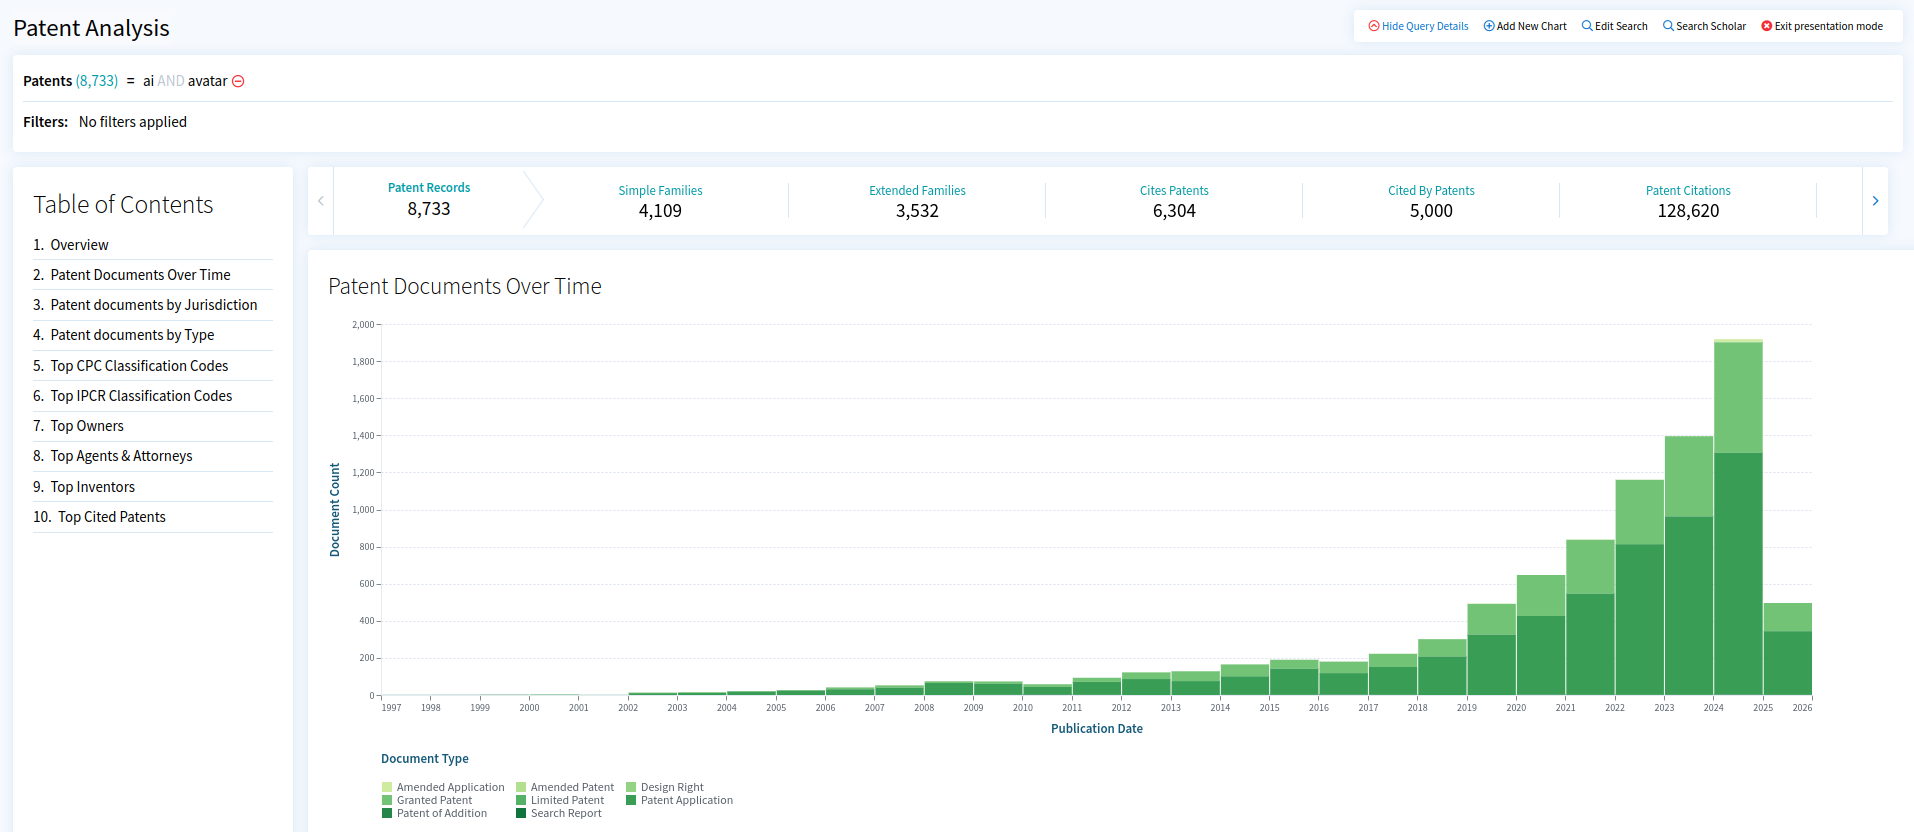
\includegraphics[width=1.0\linewidth]{images/patent-analysis.png}
    \caption{Патентный анализ}
    \label{fig:patent-analysis}
\end{figure}

\chapter{Обзор научно-технических источников информации} 

Реализация программного сервиса, связанного с обучаемыми цифровыми аватарами,
невозможна без опоры на современные научно-технические достижения
в области веб-разработки, распределённых вычислений,
хранения и обработки мультимедийных данных, а также технологий машинного обучения.
В данном разделе рассматриваются ключевые архитектурные и инфраструктурные решения,
а также программные компоненты, позволяющие реализовать сервис на практике.

\section{Концептуальные и архитектурные решения}
\subsection{Общий архитектурный паттерн. Микросервисный и монолитный подходы}

В качестве базового архитектурного паттерна
для дипломного проекта был выбран микросервисный подход.
Данный выбор обусловлен спецификой разрабатываемого приложения,
которое представляет собой комплексный сервис
с явно выраженными отдельными функциональными модулями:
интерфейсом взаимодействия с пользователями,
модулем генерации текстовых и аудиоответов,
процессом обучения моделей,
а также системой хранения и управления данными.

Микросервисная архитектура позволяет эффективно
распределить обязанности между компонентами,
разрабатывать их независимо друг от друга
и проводить параллельную работу над проектом в рамках команды.

Кроме того, такой подход значительно упрощает
процессы масштабирования.
При росте нагрузки можно увеличивать ресурсы
только для тех компонентов,
которые в этом нуждаются,
не затрагивая остальную систему.

В качестве альтернативы можно было бы рассмотреть монолитную архитектуру,
предполагающую разработку всех функций сервиса
в рамках единого приложения.
Несмотря на относительную простоту реализации на начальных этапах,
монолитное приложение имеет ряд существенных ограничений:
усложняется внесение изменений,
требующих частых релизов,
и масштабирование становится менее гибким,
так как масштабируется весь монолит целиком,
а не отдельные его части.

Кроме того, использование микросервисов упрощает
интеграцию различных технологий и фреймворков,
что особенно важно в контексте дипломного проекта,
в котором задействованы разнообразные инструменты и подходы,
такие как NLP и TTS модели,
брокеры сообщений и несколько видов баз данных.

Таким образом, микросервисная архитектура обеспечивает
необходимую гибкость, отказоустойчивость,
возможность масштабирования отдельных компонентов
и параллельную разработку в рамках команды,
что делает её оптимальным выбором в рамках дипломной разработки.

\subsection{Паттерн взаимодействия микросервисов. Хореография и оркестрация}

При построении взаимодействия между микросервисами
в рамках дипломного проекта был выбран паттерн оркестрации.
Он предполагает наличие централизованного компонента — оркестратора,
который управляет потоками данных и координирует вызовы
между отдельными модулями системы.

Такой подход хорошо подходит для систем,
в которых важна наблюдаемость,
чёткое управление последовательностью операций,
а также необходимость логирования состояния на каждом этапе обработки.

Альтернативным решением могла бы быть хореография,
где каждый микросервис действует автономно,
реагируя на события, опубликованные другими сервисами,
и самостоятельно принимая решения о своей логике работы.
Хореография более гибка и масштабируема
в условиях loosely coupled-сервисов,
однако она увеличивает сложность отладки,
снижает прозрачность процессов
и требует высокой зрелости всей архитектуры.

В контексте данного дипломного проекта,
где важны управляемость процессов,
централизованная маршрутизация запросов,
а также простота расширения и логирования,
паттерн оркестрации оказался более подходящим.

Он позволяет точно определять,
в какой момент вызывается тот или иной модуль,
а также централизованно обрабатывать ошибки
и реализовывать управление зависимостями между компонентами.

Таким образом, выбор в пользу оркестрации
обеспечивает необходимый баланс между контролем,
гибкостью и надёжностью при построении архитектуры сервиса
в рамках дипломной работы.

\subsection{Модель взаимодействия компонентов. Асинхронность, параллельность и конкурентность}

Одним из ключевых архитектурных решений
в рамках дипломной разработки стало использование асинхронного взаимодействия
между компонентами системы.
Данный подход был выбран с учётом природы выполняемых задач,
в частности генерации текстов и синтеза речи,
которые требуют значительных вычислительных ресурсов
и занимают заметное время на выполнение.

Асинхронная модель позволяет выполнять такие задачи
в фоновом режиме, не блокируя основной поток обработки,
и даёт возможность пользователю
продолжать взаимодействие с системой,
в том числе с другими аватарами,
не дожидаясь завершения ресурсоёмких операций.

Для лучшего понимания выбора архитектурной модели
необходимо кратко рассмотреть отличия между
асинхронностью, параллельностью и конкурентностью.
Асинхронность — это способ организации кода,
при котором выполнение может быть приостановлено и возобновлено позже,
что особенно эффективно в условиях операций ввода-вывода (I/O).
Параллельность же подразумевает физическое исполнение
нескольких задач одновременно, как правило — на разных ядрах процессора.
Конкурентность — более широкое понятие,
обозначающее возможность выполнения нескольких задач,
не обязательно параллельно,
но с чередованием выполнения или асинхронным управлением.

Асинхронное исполнение часто реализуется в виде событийного цикла,
в то время как параллельное — через многопоточность или многопроцессность.
Последние требуют более сложной координации и синхронизации,
что затрудняет масштабирование и отладку,
особенно в распределённой архитектуре.

В отличие от синхронного исполнения,
где каждый компонент ожидает завершения предыдущего действия,
асинхронный подход обеспечивает
более высокую отзывчивость и масштабируемость сервиса.
Синхронные вызовы проще в реализации,
но в условиях высоких задержек
или большого количества параллельных запросов
они ведут к блокировке потоков и снижению общей производительности.

Параллельное исполнение с использованием многопоточности
могло бы частично компенсировать блокировки,
однако такая реализация сложнее в обслуживании
и, забегая вперёд, стоит отметить,
что в случае с Python (язык будет подробнее рассмотрен в следующем разделе)
данный подход дополнительно осложняется ограничениями, связанными с GIL (Global Interpreter Lock),
характерным для языка программирования Python, технический выбор которого будет обоснован в последующих разделах.
Кроме того, в контексте работы с языковыми и звуковыми моделями
важно учитывать, что генерация занимает значительное время на GPU,
и в условиях параллельного запуска таких операций
быстро наступает исчерпание доступных ресурсов,
что приводит либо к очередям, либо к отказам в обработке.

Асинхронная модель позволяет более эффективно
распределять ресурсы между задачами,
обрабатывая запросы по мере готовности моделей к генерации,
а не блокируя систему в ожидании ответа от перегруженного компонента.

Таким образом, выбор асинхронного взаимодействия
в рамках дипломного проекта продиктован особенностями предполагаемой нагрузки:
интенсивные операции генерации и обучения,
непредсказуемое время отклика,
высокая параллельность пользовательских запросов
и необходимость устойчивой обработки в условиях
сетевой неопределённости и ограниченных вычислительных ресурсов.

\subsection{Модель хранения данных}
В рамках дипломной разработки рассматриваемый сервис
взаимодействует с принципиально разными типами данных,
что требует осознанного выбора подходящих систем хранения.
Ключевым источником анализа стал труд \cite{DataIntenciveDesign},
в котором систематизированы подходы к выбору хранилищ
в зависимости от характера данных и типов нагрузки.

Первым типом данных являются структурированные сущности:
информация о пользователях, профилях и параметрах аватаров,
чат-сессиях, настройках и доступах.
Для этих целей была выбрана реляционная база данных,
которая обеспечивает консистентность, связность данных
и мощный язык запросов (SQL), необходимый для аналитических задач
и построения сложных фильтров.
Альтернативой могли бы выступать документо-ориентированные СУБД,
например MongoDB, однако в данном случае
иерархическая структура с чёткими отношениями между таблицами
оказалась более подходящей.

Вторым важным типом данных являются
большие бинарные объекты — аудио- и видеоматериалы,
загружаемые пользователями для обучения аватаров.
Хранение таких файлов в реляционной базе данных
представляется неэффективным с точки зрения производительности и масштабирования.
Для этих целей было выбрано объектное хранилище,
поддерживающее интерфейс S3,
что обеспечивает совместимость с индустриальными инструментами
и удобство масштабируемого хранения.
Возможными альтернативами могли бы быть файловые хранилища
или blob-хранилища в рамках SQL-СУБД,
однако они уступают по скорости доступа,
гибкости маршрутизации и отказоустойчивости.

Наконец, особую категорию составляют
внутренние технические данные — журналы событий, логи ошибок,
статистика работы сервисов.
Эти данные имеют потоковую природу
и требуют быстрого добавления и поиска по ключу.
Для этих целей используется key-value-хранилище,
оптимизированное под работу с большим объёмом логов в режиме реального времени.
Альтернативой могла бы быть файловая система
или хранение логов в PostgreSQL,
но это создаёт избыточную нагрузку и снижает общую отзывчивость системы.

Таким образом, комбинация трёх типов хранилищ —
реляционного, объектного и ключ-значение —
обеспечивает логическую и техническую оптимальность решения задачи хранения
в условиях разнородных данных и разнообразных сценариев их использования.

\subsection{Паттерн клиентской архитектуры. Модели MPA и SPA}

В качестве модели клиентской части приложения был выбран паттерн SPA (Single Page Application), который предполагает 
однократную загрузку основного интерфейса и последующую динамическую подгрузку данных через API без полной перезагрузки 
страницы.

Выбор данного подхода обусловлен необходимостью обеспечить высокую отзывчивость и непрерывность пользовательского 
взаимодействия, особенно в условиях частых обращений к функциональности, связанной с управлением аватарами и обменом 
сообщениями в режиме реального времени. Такой сценарий требует гибкой клиентской логики и быстрого отклика интерфейса, что 
достигается за счёт исключения циклов полной перерисовки страницы.

Фронтенд построен с опорой на современные принципы реактивного взаимодействия, реализованные средствами, не требующими 
использования тяжёлых фреймворков. Это позволило упростить архитектуру, сохранить единообразие технологического стека и 
сократить затраты времени на разработку — особенно актуальные факторы в условиях ограниченных ресурсов дипломного проекта.

Альтернативой SPA могла бы стать модель MPA (Multi Page Application), при которой каждое взаимодействие пользователя приводит 
к загрузке новой страницы с серверным рендерингом содержимого. Несмотря на простоту реализации, данный подход менее эффективен 
в сценариях, требующих высокой интерактивности и поддержки многосессионного взаимодействия.

Таким образом, архитектура SPA была выбрана как наиболее подходящая, обеспечивая баланс между 
интерактивностью пользовательского интерфейса и эффективностью разработки.

\section{Программные средства и технологии реализации}
\subsection{Выбор языка программирования}

Ключевым техническим решением в рамках дипломной разработки
стал выбор языка программирования Python
в качестве основного инструмента для реализации серверной логики.

Python был выбран по совокупности следующих причин:
широкая поддержка асинхронного программирования,
богатая экосистема библиотек для работы с данными,
интеграция с фреймворками машинного обучения,
а также высокая читаемость и скорость разработки,
что особенно важно в условиях ограниченного времени и ресурсов.

Дополнительно, наличие развитых средств работы
с языковыми и звуковыми моделями (таких как библиотеки HuggingFace,
Transformers, Torchaudio и др.) делает Python
естественным выбором для построения сервисов,
основанных на обработке естественного языка и синтезе речи.

В качестве возможных альтернатив могли бы рассматриваться
языки с более высокой производительностью — например, Go или Rust,
однако в контексте дипломного проекта ключевым критерием
является не максимальная эффективность исполнения,
а возможность быстрой реализации, прототипирования и интеграции
с существующими ML-инструментами.

Кроме того, Python активно используется в академической среде,
что облегчает повторяемость, демонстрацию и возможное масштабирование решения
в дальнейшем, в том числе на инфраструктуре облачных сервисов,
таких как Google Colab, Kaggle.

Выбор Python, таким образом, органично вписывается
в общую архитектуру разрабатываемого сервиса:
его асинхронная модель исполнения сочетается
с выбранным серверным фреймворком и системой обмена сообщениями,
а гибкость и выразительность языка
позволяют эффективно реализовать как управляющую логику,
так и интеграцию с компонентами машинного обучения.

\subsection{Веб интерфейс}

При выборе технологии для реализации веб-интерфейса
в рамках настоящей выпускной квалификационной работы
решающее значение имели два основных аспекта:
ограниченный опыт участников команды
с использованием современных JavaScript-фреймворков
и стремление к технологической унификации проекта
с использованием единого языка программирования.

Исходя из этих условий, было принято решение
о выборе библиотеки FastHTML, написанной на языке Python,
которая предоставляет средства для генерации HTML-разметки
и интеграции с библиотекой HTMX.
Последняя представляет собой лёгкую JavaScript-библиотеку,
позволяющую динамически обновлять отдельные элементы страницы
посредством асинхронных HTTP-запросов,
исключая необходимость полной перезагрузки веб-страницы.

Подобное техническое решение позволило обеспечить
интерактивность пользовательского интерфейса
без привлечения более сложных и ресурсоёмких клиентских фреймворков,
что существенно упростило процессы разработки и последующего сопровождения.
Минималистичный подход к реализации веб-интерфейса
особенно оправдан в контексте проекта,
где основное внимание уделяется реализации серверной логики,
интеграции моделей машинного обучения и обработки данных.

В качестве альтернативы рассматривалась возможность использования
современных клиентских фреймворков, таких как React, Vue или Angular.
Несмотря на их обширные функциональные возможности
и развитую экосистему, применение данных инструментов
требовало бы освоения специфических технологий (например, JSX, шаблоны Vue),
создания дополнительной инфраструктуры сборки и управления зависимостями,
что существенно усложнило бы архитектуру и повысило нагрузку на разработчиков.

Дополнительным недостатком использования таких решений
стало бы неизбежное разделение проекта
на две отдельные части (клиентскую и серверную),
требующие различных инструментов, языков и процессов интеграции,
что негативно повлияло бы на простоту сопровождения
и целостность проекта в условиях ограниченных ресурсов
и учебной специфики работы.

Таким образом, выбор технологии FastHTML в сочетании с HTMX
представляется наиболее целесообразным в рамках данной работы,
обеспечивая оптимальное сочетание интерактивности интерфейса
и простоты разработки и сопровождения.

\subsection{Серверная часть. Оркестратор}

В основе серверной архитектуры дипломного проекта
лежит компонент-оркестратор, реализованный на базе библиотеки FastAPI \cite{Fastapi}.
Выбор FastAPI был обусловлен рядом преимуществ,
ключевыми среди которых являются высокая производительность
и полная поддержка асинхронного исполнения,
что обеспечивает эффективную обработку большого количества одновременных запросов
в условиях интенсивной сетевой и вычислительной нагрузки.

В качестве альтернативных решений рассматривались
популярные серверные фреймворки Django REST Framework и Flask.
Однако оба решения ориентированы преимущественно
на синхронную модель исполнения,
что делает их менее подходящими в контексте проекта,
где значительная часть операций связана с взаимодействием
между микросервисами и внешними асинхронными источниками данных.

В частности, Flask отличается простотой и минимализмом,
но требует дополнительных усилий при построении масштабируемой архитектуры,
а также не обладает встроенными средствами интеграции
с асинхронной обработкой, что ограничивает его применимость
в высоконагруженных распределённых системах.

Django REST Framework, в свою очередь,
является мощным и функциональным инструментом,
но его асинхронные возможности находятся на этапе развития
и не позволяют достичь той же степени гибкости и производительности,
которую предоставляет FastAPI.

Кроме того, важным преимуществом FastAPI является
отсутствие жёстких ограничений на структуру проекта,
что позволяет свободно организовывать взаимодействие между модулями,
интегрировать внешние хранилища, брокеры сообщений
и другие инфраструктурные компоненты без необходимости
следовать строго заданной архитектурной модели.

Таким образом, использование FastAPI в качестве
основного инструмента реализации оркестратора
представляется наиболее обоснованным решением,
соответствующим требованиям производительности, масштабируемости
и гибкости, предъявляемым к современным микросервисным приложениям
в условиях дипломного проектирования.

\subsection{Серверная часть. Модуль работы с языковой и звуковой моделью}

Одним из ключевых компонентов серверной архитектуры
является модуль генерации, отвечающий за формирование текстовых и аудиоответов
в ходе взаимодействия пользователя с аватаром.
Модуль функционирует по асинхронной модели,
обеспечивая выполнение ресурсоёмких операций вне основного цикла обработки
и получая команды от оркестратора посредством брокера сообщений,
реализующего принцип FIFO (first in, first out).

В качестве основной технологической базы
для построения языковых и звуковых моделей
были выбраны открытые библиотеки и модели
из экосистемы HuggingFace \cite{HugginFaceTransformersLib}.
Данный выбор обусловлен высоким уровнем зрелости инструментов,
поддержкой современного стекa NLP и TTS-технологий,
а также наличием предварительно обученных моделей
и инфраструктуры для дообучения и тонкой настройки.

Одним из важнейших преимуществ HuggingFace
является открытость исходного кода и соблюдение
свободных лицензий, что позволяет исключить зависимость
от коммерческих поставщиков и обеспечивает возможность
развёртывания модели в полностью контролируемой среде.
Кроме того, использование данных инструментов
снижает финансовые издержки на этапе разработки
и делает проект более устойчивым к изменениям внешней среды.

В качестве альтернативных решений могли бы рассматриваться
облачные сервисы от крупных вендоров, таких как Google Cloud (Dialogflow, Text-to-Speech),
Amazon Web Services (Polly, Lex), Microsoft Azure и др.
Несмотря на высокую точность и удобство интеграции,
эти решения обладают рядом проблем, которые включают в себя ограниченную доступность в отдельных регионах,
зависимость от внешнего API, стоимость при масштабируемом использовании,
а также ограниченные возможности кастомизации моделей под специфические задачи.

В контексте настоящей дипломной работы,
где важны автономность, воспроизводимость и контроль над конфигурацией,
использование локальных open-source решений
представляется наиболее рациональным и перспективным подходом.

Одной из главных задач для реализации пайплайнов обучения и генерации является выбор языковой модели. Для оценки производительности различных вариантов LLM был выбран ряд общепринятых бенчмарков, которые позволяют объективно оценить способности моделей от задач на базовые знания и логику до качества диалога и мультиязычности. Определяющими стали:
\begin{itemize}
    \item MMLU (Massive Multitask Language Understanding) — бенчмарк, который включает задачи из 57 различных академических дисциплин \cite{Wang2024MMLUPro};
    \item Russian SuperGLUE — аналог англоязычного SuperGLUE адаптированный под русский язык, включающий в себя тесты на классификацию, парное сопоставление текстов, логические выводы и пр. \cite{Fenogenova2022RussianSuperGLUE};
    \item MERA (Multilingual Evaluation of Reasoning Abilities) — относительно новый бенчмарк, состоящий из 21 задания по разным навыкам модели. Он позволяет выявить, насколько хорошо модель справляется с выводами вне англоязычного контекста \cite{Fenogenova2024MERA};
    \item Chatbot Arena — представляет собой систему парных сравнений моделей, где пользователи выбирают между ответами двух анонимных систем, что позволяет выявить предпочтения людей в реальном общении \cite{Chiang2024ChatbotArena};
    \item LIBRA (Linguistically Informed Benchmark for Russian AI)  — оценивает качество LLM именно в контексте русского языка, проверяя на синтаксический анализ, морфологию, семантику и другое \cite{Xu2024Libra}.
\end{itemize}
Проанализировав общую картину по всем бенчмаркам было выделено три серии открытых языковых моделей, которые показали высокие показатели: LLaMA \cite{Grattafiori2024Llama3}, Mistral \cite{Jiang2023Mistral7B}, Qwen \cite{Yang2025Qwen3} и DeepSeek \cite{DeepSeekAI2025DeepSeekV3}, имеющий наивысшие оценки.
LLM семейства LLaMA, разработанные Meta AI, имеют хороший результат в задачах понимания контекста. Mistral обладает высокой эффективностью за счет своей компактности. Qwen, разработанная Alibaba Cloud, обладает высоким качеством генерации при относительно небольшом количестве параметров. Главным их преимуществом является открытая архитектура, что позволяет использовать их в пользовательских и научных проектах. Однако, важно отметить, что данные, на которых обучались эти модели, в основном ориентированы на английский язык, поэтому из-за наличия небольшого количества текста на других языках в их наборах обучающих данных их общая производительность имеет отрицательных эффект при генерации на русском.
Отдельно стоит выделить модель DeepSeek, которую разработала китайская группа исследователей. Несмотря на то, что она в своем обучающем датасете имеет преимущественно китайские и английские текста, ее архитектура и объем позволяют ей достигать лидирующих позиций в большинстве бенчмарков.
Русский язык является одним из наиболее ресурсоемких языков с точки зрения морфологии, синтаксиса и семантики, что требует от LLM языковой адаптации и богатого лингвистического представления в наборах данных. Для решения этой проблемы были разработаны MTS AI, GigaChat и YandexGPT, которые демонстрируют высокое качество генерации, превосходя своих флагманских конкурентов,
ориентированных на английский язык, в том, что касается обработки и генерации текста на русском, но имеют закрытый исходный код, что делает невозможность их использование в рамках научного проекта. Поэтому высокой популярностью пользуются открытые модели, среди которых можно выделить серии Saiga \cite{Gusev2025RULM}, ruGPT \cite{Zmitrovich2023RussianLMs}, ruadapt \cite{Tikhomirov2024LEP} и Vikhr \cite{Nikolich2024Vikhr}. Они были дообучены на базе лидирующих англоязычных LLM и дополнительно настроены для улучшения генерации и понимания текста именно в русскоязычном контексте.
В таблице \ref{tab:pingpong} представлены средние значения по бенчмарку PingPong \cite{Gusev2025PingPong}, оценивающим языковые модели в их способности поддерживать многораундовую беседу, сохраняя выбранную роль и персону. Как из нее видно LLM семейства Saiga входят в число лидеров, что делает ее оптимальным выбором для задачи генерации текста в речевом стиле конкретного человека.


\begin{table}[h!]
\centering
\resizebox{\textwidth}{!}{
\begin{tabular}{|c|c|c|c|}
\hline
 Модель $\backslash$ PingPong бенчмарк & Average Score & Average Score \\
\hline
deepseek\_v3\_0324                 & 4.79±0.04 & 4.93 \\
\hline
deepseek\_v3               & 4.65±0.06 & 4.79 \\
\hline
	
sainemo\_remix\_12b               & 4.61±0.07 & 4.64 \\
\hline
saiga\_yandexgpt\_8b    & 4.69±0.05 & 4.71 \\
\hline
	
saiga\_nemo\_12b\_v3                 & 4.68±0.06 & 4.63 \\
\hline
mistral\_nemo\_vikhr\_dostoevsky\_slerp\_12b                   & 4.55±0.06 & 4.59 \\
\hline
saiga\_gemma3\_12b             & 4.73±0.07 & 4.74 \\
\hline
\end{tabular}
}
\caption{Сравнение моделей по бенчмарку PingPong}
\label{tab:pingpong}
\end{table}

\subsection{Серверная часть. Технология распознавания речи}
Для преобразования аудиоданных в текст в рамках пайплайна обучения использовалась модель автоматического распознавания речи Whisper, разработанная компанией Open AI \cite{Zhao2024WhisperPMFA}. Она является представителем open-source систем ASR (Automatic Speech Recognition), основанную на архитектуре трансформеров и обученную на большом объеме аудиоматериалов, включающих различные интервью, лекции, подкасты, видеоконтент. Благодаря этому Whisper хорошо справляется с переводом потенциальных источников информации для сбора датасета под конкретного человека.
В качестве альтернативных решений рассматривались облачные сервисы, такие как Google Speech-to-Text, однако их применение ограничено лицензионными условиями и необходимостью постоянного интернет-соединения. Кроме того, была проанализирована модель Wav2Vec 2.0 \cite{Baevski2020Wav2Vec2}, разработанная Facebook AI Research, которая демонстрирует высокую точность на английском языке, но требует дополнительного дообучения для русского, что значительно усложняет ее интеграцию в проект и увеличивает требования к вычислительным ресурсам.
Для извлечения аудиодорожки из видеофайлов выбрана библиотека MoviePy, которая имеет удобный и простой интерфейс, что упрощает процесс программной реализации данного этапа пайплайна. Данный модуль является удобной надстройкой над библиотекой FFmpeg, упрощая функции нарезки, конкатенации, преобразования форматов, обеспечивая высокий уровень абстракции. 



\subsection{Серверная часть. Брокер сообщений}

Для организации взаимодействия между микросервисами
в архитектуре дипломного проекта применяется брокер сообщений,
играющий ключевую роль в обеспечении асинхронной коммуникации
и устойчивости системы к пиковым нагрузкам.

В качестве основного инструмента был выбран Apache Kafka \cite{ApacheKafka},
широко распространённая распределённая платформа
для обработки потоков данных в реальном времени.
Kafka обеспечивает высокую пропускную способность,
гарантированную доставку сообщений,
а также масштабируемость за счёт распределённой архитектуры,
что делает её оптимальным решением для сервисов,
требующих надёжной и непрерывной передачи данных между компонентами.

Выбор Kafka также обоснован её зрелостью,
широкой поддержкой в сообществе и богатой документацией,
а также наличием опыта работы с данной системой в команде,
что позволило сократить время на внедрение и конфигурацию.

В качестве альтернатив могли бы быть использованы
RabbitMQ — брокер с поддержкой расширенных шаблонов маршрутизации сообщений,
или Memphis — более молодой, но активно развивающийся инструмент
с удобным интерфейсом и низким порогом входа.
Тем не менее, в условиях проекта, ориентированного на
обработку ресурсоёмких задач и высокую частоту межсервисных взаимодействий,
Kafka продемонстрировала наибольшую пригодность благодаря своей отказоустойчивости
и способности обрабатывать большие объёмы сообщений в режиме реального времени.

Таким образом, применение Apache Kafka
представляется технически обоснованным решением,
соответствующим требованиям надёжности, масштабируемости и производительности,
необходимым для устойчивой работы распределённого сервиса
в рамках дипломного проекта.

\subsection{Инфраструктура и развертывание}

Микросервисная архитектура, выбранная в рамках дипломной разработки,
предполагает наличие большого числа взаимосвязанных компонентов,
каждый из которых выполняет строго определённую функцию
и может развиваться независимо от остальных.
Такая модульность увеличивает гибкость и масштабируемость системы,
но одновременно усложняет процессы развертывания, настройки и сопровождения.

Для минимизации издержек на конфигурацию окружения и унификацию подходов
к развертыванию различных сервисов было принято решение
использовать технологию контейнеризации на основе Docker \cite{Docker}.
Docker предоставляет изолированную среду выполнения
для каждого из компонентов, позволяя гарантировать
одинаковое поведение приложений вне зависимости от целевой платформы.

Дополнительно применяется инструмент Docker Compose,
обеспечивающий декларативное описание всей системы
и автоматизацию процессов сборки, настройки и запуска сервисов
в едином командном интерфейсе.
Такой подход значительно упрощает работу с инфраструктурой
на этапе разработки, тестирования и демонстрации,
что особенно важно в условиях дипломного проектирования,
где критичны воспроизводимость и предсказуемость поведения среды.

В качестве альтернативы контейнеризации
могло бы рассматриваться использование виртуальных машин.
Однако данный подход предполагает более высокие накладные расходы,
меньшую гибкость в масштабировании
и требует отдельной настройки каждой инстанции системы,
что затрудняет управление и автоматизацию развёртывания.

Таким образом, применение Docker и связанных с ним инструментов
позволило выстроить устойчивую и удобную в сопровождении инфраструктуру,
оптимально подходящую для микросервисной архитектуры,
реализуемой в рамках дипломного проекта.

\subsection{Итог по архитектуре}

\begin{table}[h!]
\centering
\resizebox{\textwidth}{!}{
\begin{tabular}{|p{3.3cm}|p{3.1cm}|p{3.3cm}|p{6.2cm}|}
\hline
\textbf{Область} & \textbf{Выбрано} & \textbf{Альтернативы} & \textbf{Ключевые аргументы выбора} \\
\hline
Архитектурный паттерн & Микросервисы & Монолит & 
Гибкое масштабирование по компонентам.
База для параллельной работы команды.
Упрощённая интеграция разнородных технологий \\
\hline
Взаимодействие микросервисов & Оркестрация & Хореография &
Требуется центральный контроль,
единый маршрутизатор запросов,
упрощённый контроль точек отказав \\
\hline
Модель исполнения & Асинхронность & Синхронность или многопоточность &
Высокая отзывчивость при I/O-нагрузке.
Нет затрат на синхронизацию потоков.
\\
\hline
Модель хранения & RDBMS + S3 Object Store + Key–Value & Только SQL.  Только NoSQL.  Локальная файловая система. &
Выбор нативно продиктован формой нагрузки
и видом данных для хранения.
Структурные данные в SQL.
Крупные бинарные объекты — в S3.
Логи и временные статусы — в KV-хранилище.
\\
\hline
Клиентская архитектура & SPA & MPA &
Непрерывный UX, частые
AJAX-запросы для диалогов.
\\ 
\hline
\end{tabular}
}
\caption{Архитектурные решения и обоснование выбора}
\end{table}


\begin{table}[h]
\centering
\resizebox{\textwidth}{!}{
\begin{tabular}{|p{3cm}|p{3.2cm}|p{3.3cm}|p{6cm}|}
\hline
\textbf{Компонент} &
\textbf{Технология} &
\textbf{Альтернативы} &
\textbf{Причины выбора} \\ \hline
Язык программирования & Python & Go &
Широкая экосистема 
как для веб-разработки
так и для ML
\\
\hline
Оркестратор (API) & FastAPI & Django REST (DRF), Flask &
Полноценный async.
Минимальные требования
к структуре проекта от фреймворка
\\
\hline
Модуль NLP / TTS & HuggingFace Transformers / TTS & Google Cloud TTS, Azure Cognitive, ElevenLabs&
Открытый код библиотек,
бесплатный доступ к необходимому 
спектру облачного функционала
\\
\hline
Брокер сообщений & Apache Kafka & RabbitMQ; Memphis &
Опыт работы с платформой,
так как в контексте работы
от брокера требуется базовый функционал 
\\
\hline
Веб-интерфейс & FastHTML + HTMX & React, Vue, Angular &
Единый язык проекта.
Отсутствие опыта у команды в работе с 
JS-фреймворками
\\
\hline
Развёртывание & Docker + Docker Compose & Виртуальные машины &
Унификация интерфейса для локальной разработки,
упрощенные условия для потенциального 
деплоя продукта
\\
\hline
\end{tabular}
}
\caption{Выбранный технологический стек и рассмотренные альтернативы}
\end{table}

\chapter{Постановка задачи} 
Основной целью разрабатываемого сервиса является предоставление пользователям удобного и понятного интерфейса для 
взаимодействия с цифровыми двойниками реальных личностей — интеллектуальными аватарами. Сервис должен позволять не только 
вести диалог с аватаром посредством текстового и аудио общения, но и иметь возможность полноценного обучения аватара с 
использованием широкого спектра материалов, таких как тексты, аудио и видео. В результате аватар должен максимально точно 
воспроизводить индивидуальные особенности манеры общения и эмоционального отклика выбранного человека.

Для достижения поставленной цели необходимо реализовать следующие технические требования к минимальной конфигурации сервиса:

\begin{itemize}
\item Разработка веб-интерфейса, предоставляющего пользователям возможность 
взаимодействовать с созданными аватарами, задавать им вопросы и получать текстовые и аудио 
ответы в реальном времени.
\item Реализация удобного и интуитивного интерфейса для процесса обучения аватаров, который 
позволит пользователям загружать материалы различных форматов (тексты, аудио и видеозаписи) 
для последующей обработки и обучения моделей.
\item Обеспечение стабильности и надежности процесса обучения языковых и звуковых моделей, 
который является наиболее ресурсоёмкой частью работы сервиса и требует эффективного 
управления вычислительными ресурсами.
\item Поддержка возможности интеграции дополнительных источников данных и сторонних 
сервисов, таких как социальные сети и мессенджеры, для получения дополнительных материалов, 
обогащающих процесс обучения аватаров.
\item Реализация механизма хранения и управления данными разного типа и формата, включая 
метаданные аватаров, пользовательские данные, текстовые и аудио материалы для обучения, а 
также системные логи.
\end{itemize}

Таким образом, итоговая архитектура должна обеспечивать гибкость, производительность и 
простоту использования, позволяя пользователям не только взаимодействовать с виртуальными 
аватарами, но и активно участвовать в процессе их создания и улучшения.
\chapter{Сущность решения задачи}

Описанные выше технические требования нашли своё отражение в сущности решения задачи предоставления удобного сервиса для создания, обучения и общения с цифровыми двойниками. Решение было дифференцированно на несколько независимых сущностей, каждая из которых была материализованна в соответствующие компоненты системы.

\section{Компоненты решения}
\subsection{Веб интерфейс}
Веб интерфейс отвечает за взаимодействие с пользователем и именно с его помощью пользователь будет посылать запросы внутрь системы. Так же этот компонент системы будет отвечать за то, чтобы потребитель получил результат работы сервиса в удобном и интуитивно понятном формате.

\subsection{Бекэнд}
Бекэнд необходим для запуска запрошенных процедур со стороны пользователя через веб интерфейс. Помимо этого компонент занимается оркестрацией всего сервиса, первичной предобработкой данных, полученных от пользователя и возврата промежуточных и итоговых результатов работы сервиса.

\subsection{Реляционная база данных}
Реляционная база данных предоставляет среду для хранения метаданных пользователя и аватаров, состояния системы, а так же быстрого поиска, вставки и модификации этих данных. Так же для корректной работы системы необходимо, чтобы данные оставались валидными в условиях конкурентного исполнения, что так же является зоной ответственности этого компонента.

\subsection{ML сервис}
ML сервис занимается непосредственным обучением моделей и генерацией данных для создания ответа и его озвучки на запрос пользователя с помощью ранее обученных моделей. Причем после обучения модели для конкретного цифрового двойника этот сервис должен обеспечить возможность быстрого взаимодействия без повторного обучения модели при последующем обращении. Поэтому данный компонент контролирует сохранение и выгрузку весов моделей, полученных в результате процедуры обучения на пользовательских данных.

\subsection{Брокер сообщений}
Брокер сообщений является сердцем всей системы, так как он предоставляет отказоустойчивую и отзывчивую среду для организации межкомпонентного взаимодействия системы.

\subsection{S3 хранилище}
S3 хранилище обеспечивает хранение, обновление и удаление больших по объему данных, которые не укладываются или их хранение является неэффективным в контексте реляционных баз данных.

\section{Алгоритм взаимодействия}

\subsection{Процедуры регистрации и аутентификации пользователя}
Нельзя забывать о том, что мы работаем с данными пользователя, значит, нельзя забывать и о конфиденциальности. Поэтому помимо непосредственного решения поставленной задачи необходимо позаботиться о защищенности данных. Самый простой и надежный способ сделать это - добавить функционал аутентификации пользователей. Таким образом сервис сможет гарантировать, что доступ к данным будет оставаться только у владельца соответствующей учетной записи. На диаграмме процесса регистрации и аутентификации (рис. \ref{fig:uf-log-or-reg}) описаны шаги, которые пользователь проходит от момента перехода на веб страницу сервиса до перехода в личный кабинет, который предоставляет интерфейс по управлению аватарами.

\begin{figure}[h!]
     \centering
     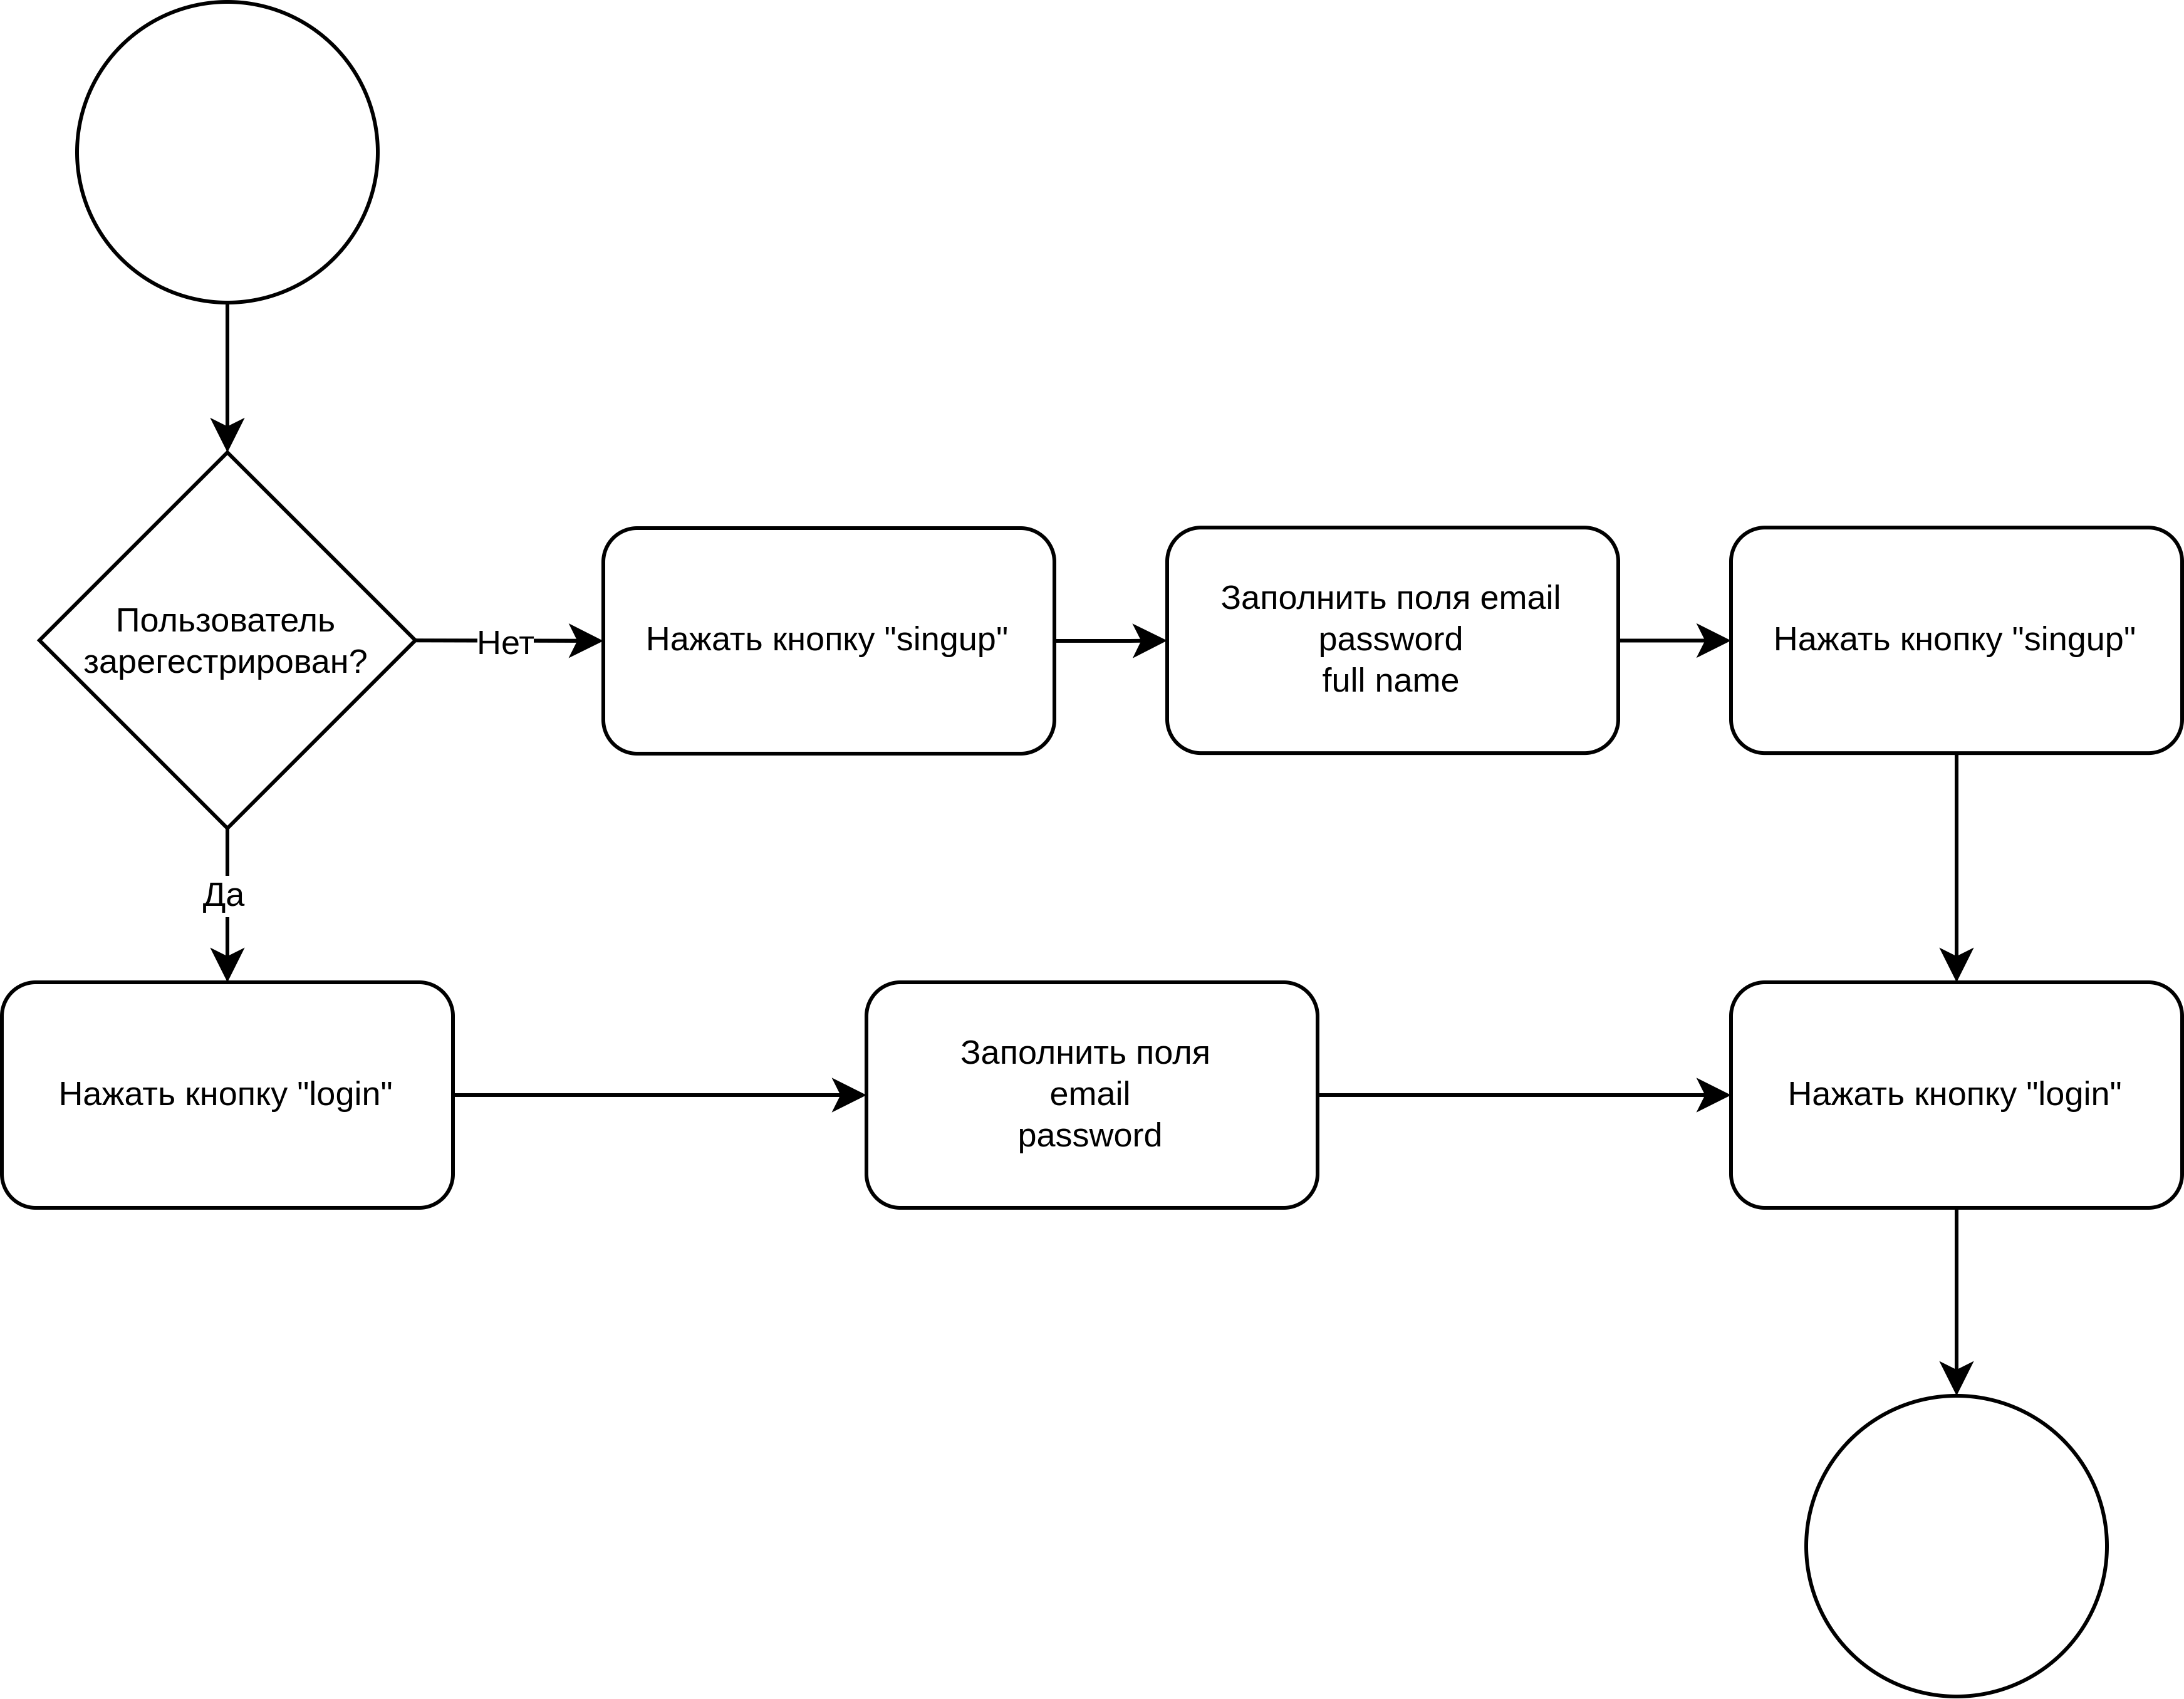
\includegraphics[width=1.0\linewidth]{images/UF-login-or-reg.png}
     \caption{User flow диаграмма процесса регистрации или авторизации}
     \label{fig:uf-log-or-reg}
\end{figure}

\subsection{Процедура обучения}
Решение имеет микросервисную архитектуру. Это значит, что весь сервис разбит на ряд независимых с точки зрения физического расположения компонент, а взаимодействие между ними происходит через сеть с помощью брокера сообщений. На диаграмме обучения аватара (рис. \ref{fig:uml-train}) представлены основные сообщения и события, которые происходят в системе для получения желаемого результата. Так же на user flow диаграмме (рис. \ref{fig:uf-train}) показано какие именно действия производит пользователь для обучения существующего или создания и обучения нового аватара.

 \begin{figure}[h!]
     \centering
     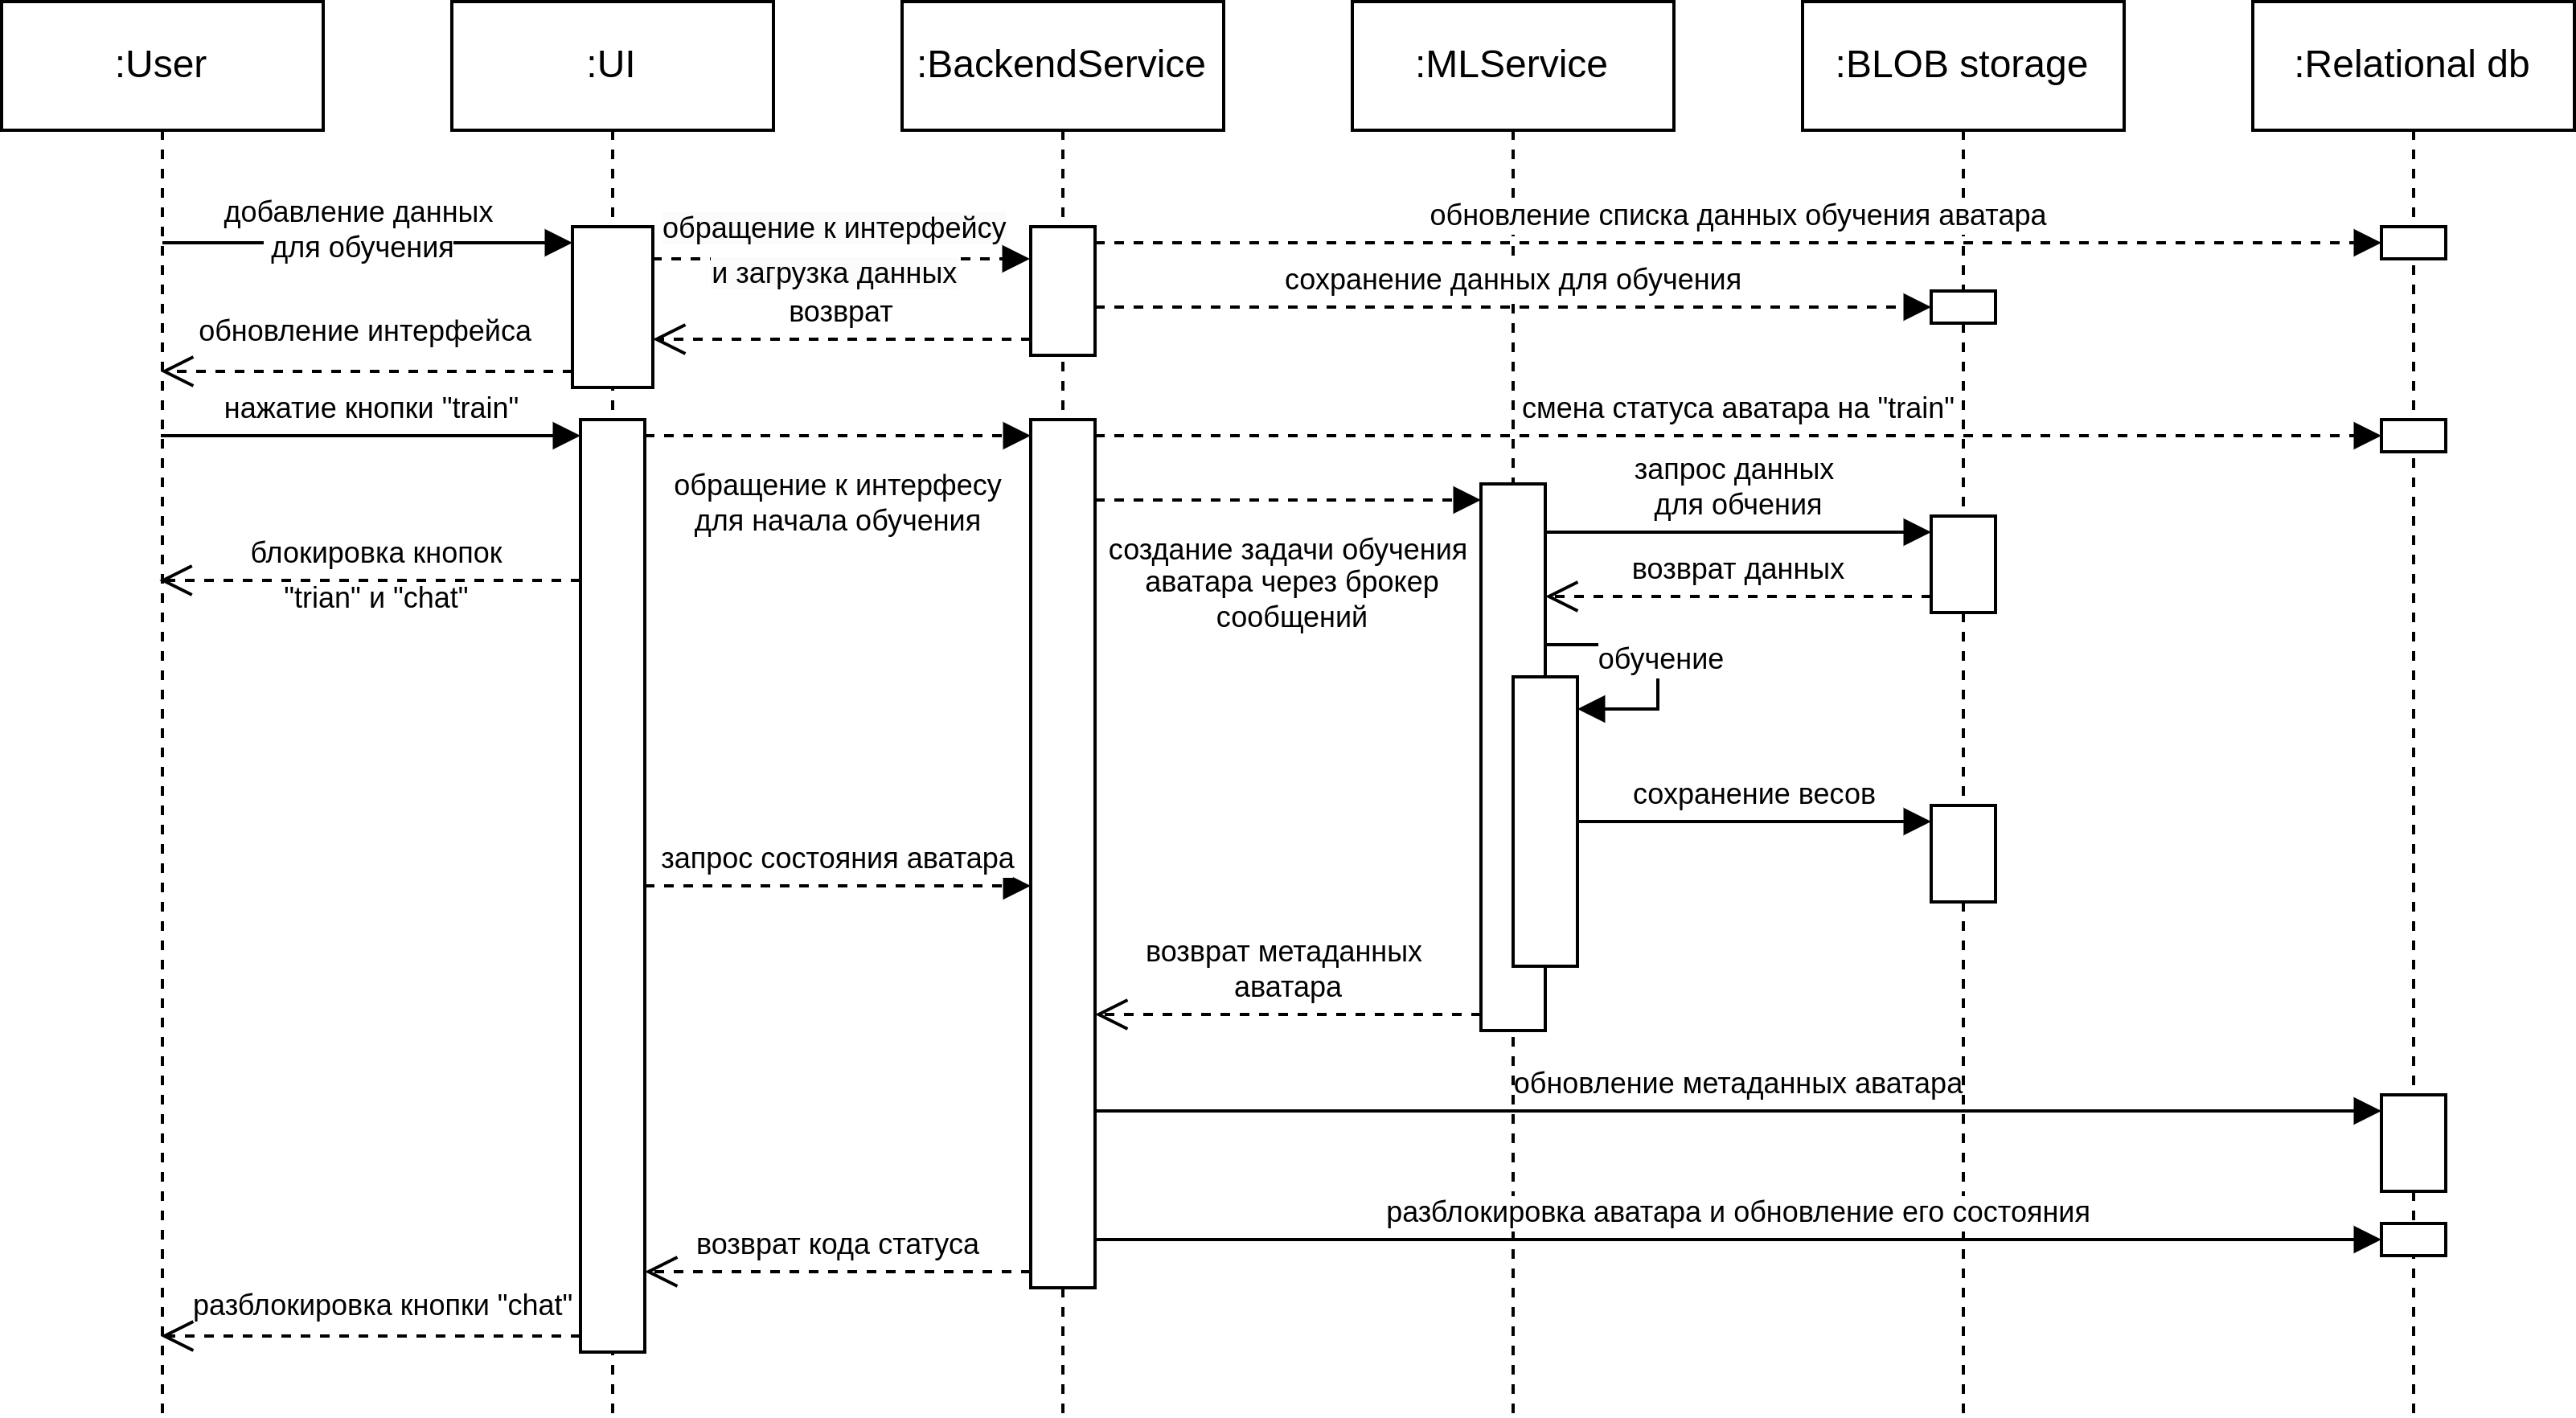
\includegraphics[width=1.0\linewidth]{images/uml-train-rus.png}
     \caption{UML-диаграмма процесса обучения}
     \label{fig:uml-train}
 \end{figure}
 \begin{figure}[h!]
    \centering
    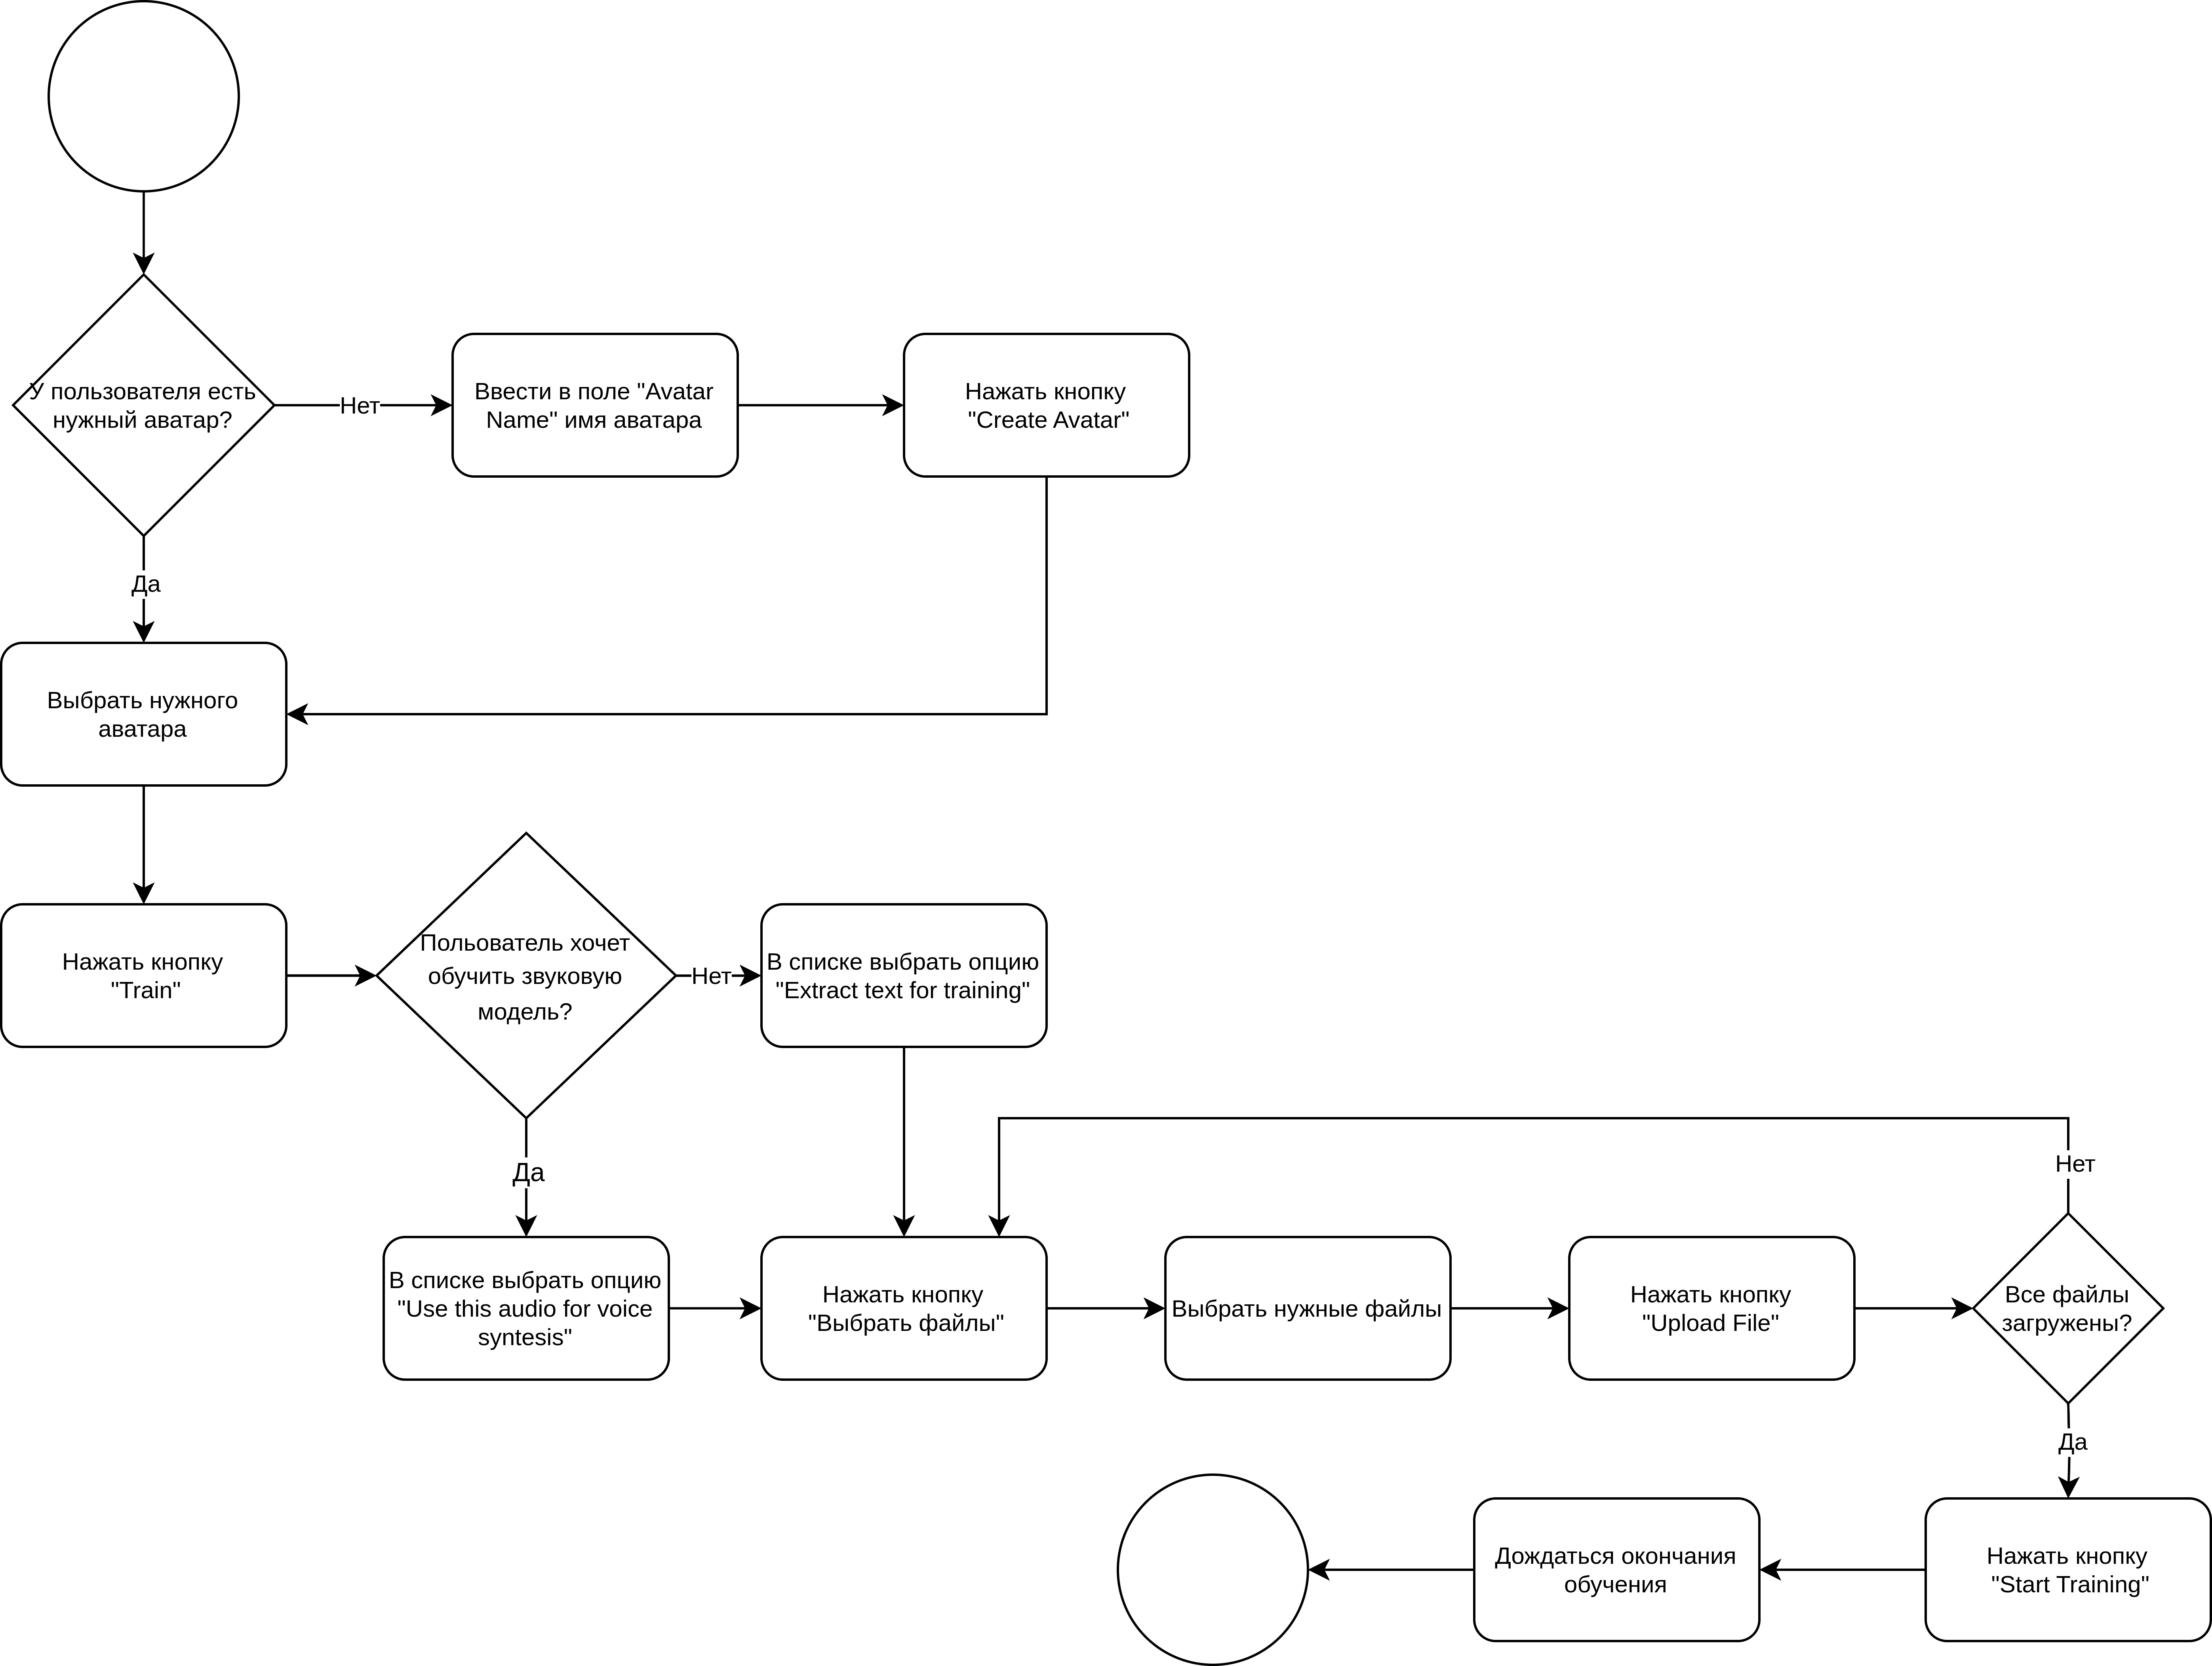
\includegraphics[width=1.0\linewidth]{images/UF-train-avatar.png}
    \caption{User flow диаграмма процесса обучения (пользователь уже выполнил вход)}
    \label{fig:uf-train}
\end{figure}

\subsection{Процедура взаимодействия с аватаром}
Аналогично процессу обучения на диаграмме процесса генерации (рис. \ref{fig:uml-inference}) отражены основные сообщения и события, через которые проходит система для предоставления пользователю сгенерированного текстового ответа и его озвучки на запрос. Аналогично представлен путь, через который проходит пользователь для создания запроса и получения ответа на user flow диаграмме (рис. \ref{fig:uf-chat-with-avatar})

 \begin{figure}[h!]
     \centering
     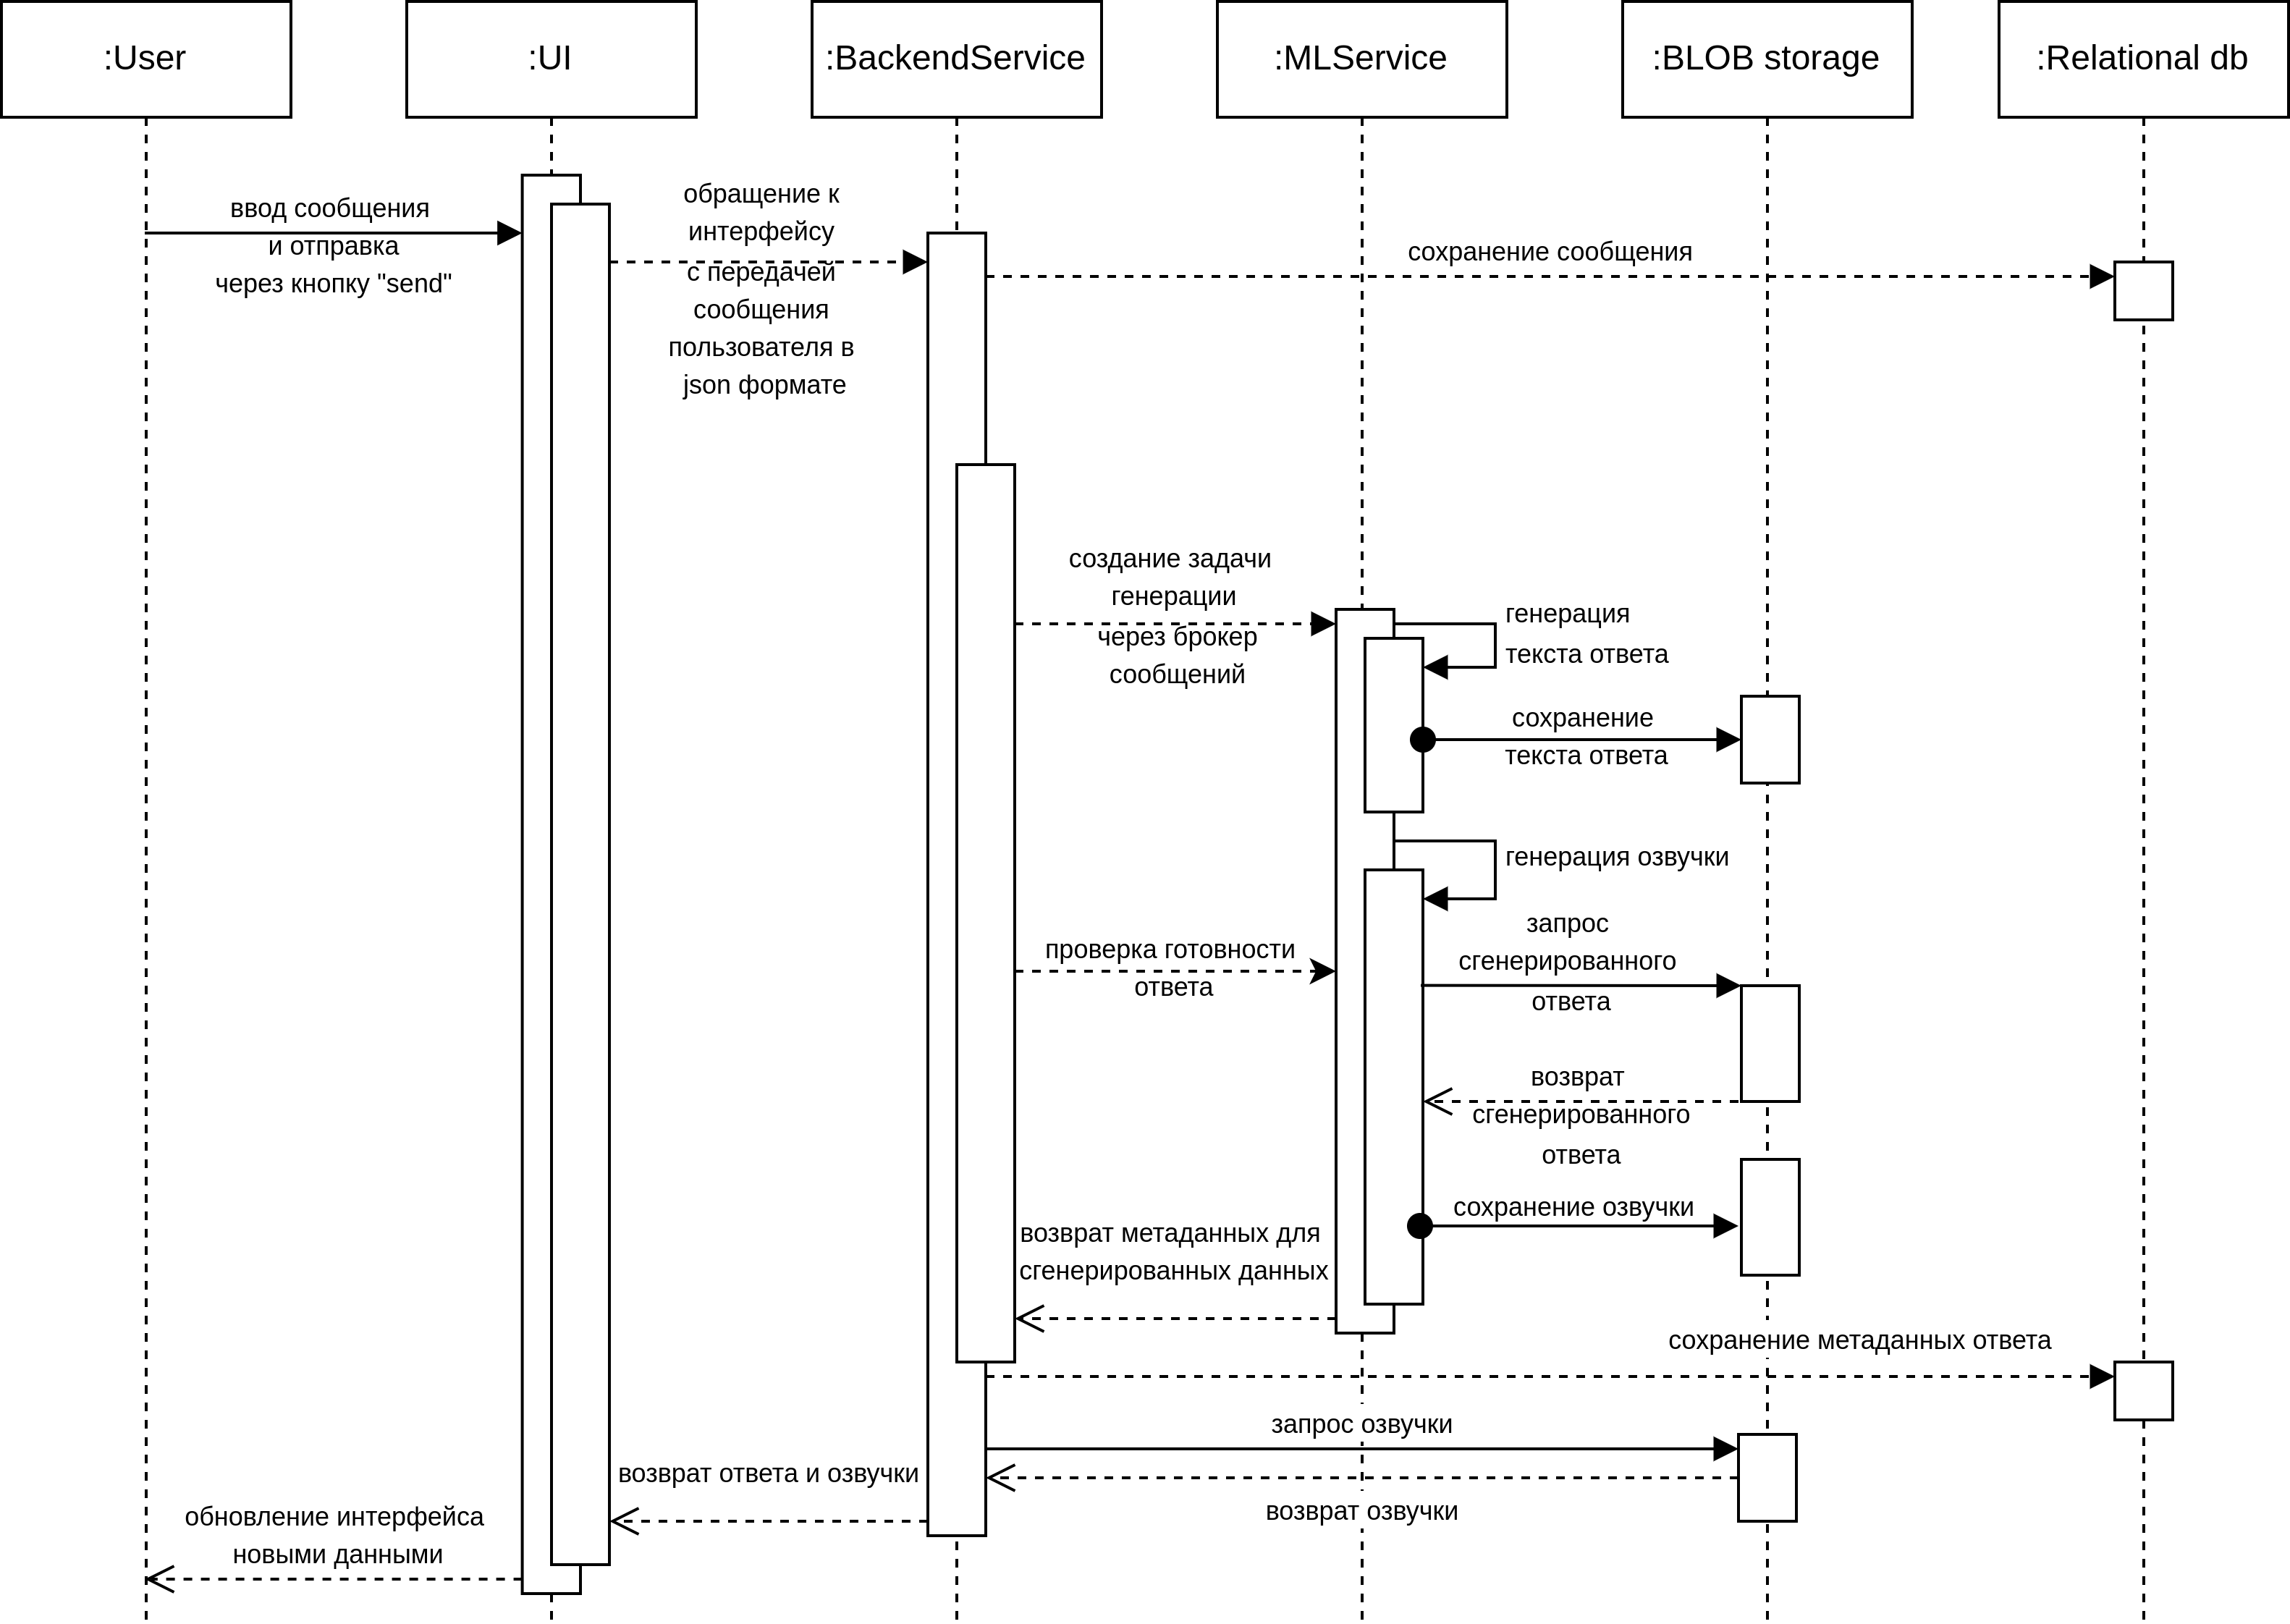
\includegraphics[width=1.0\linewidth]{images/uml-inference-rus.png}
     \caption{UML-диаграмма процесса генерации}
     \label{fig:uml-inference}
 \end{figure}
 \begin{figure}[h!]
    \centering
    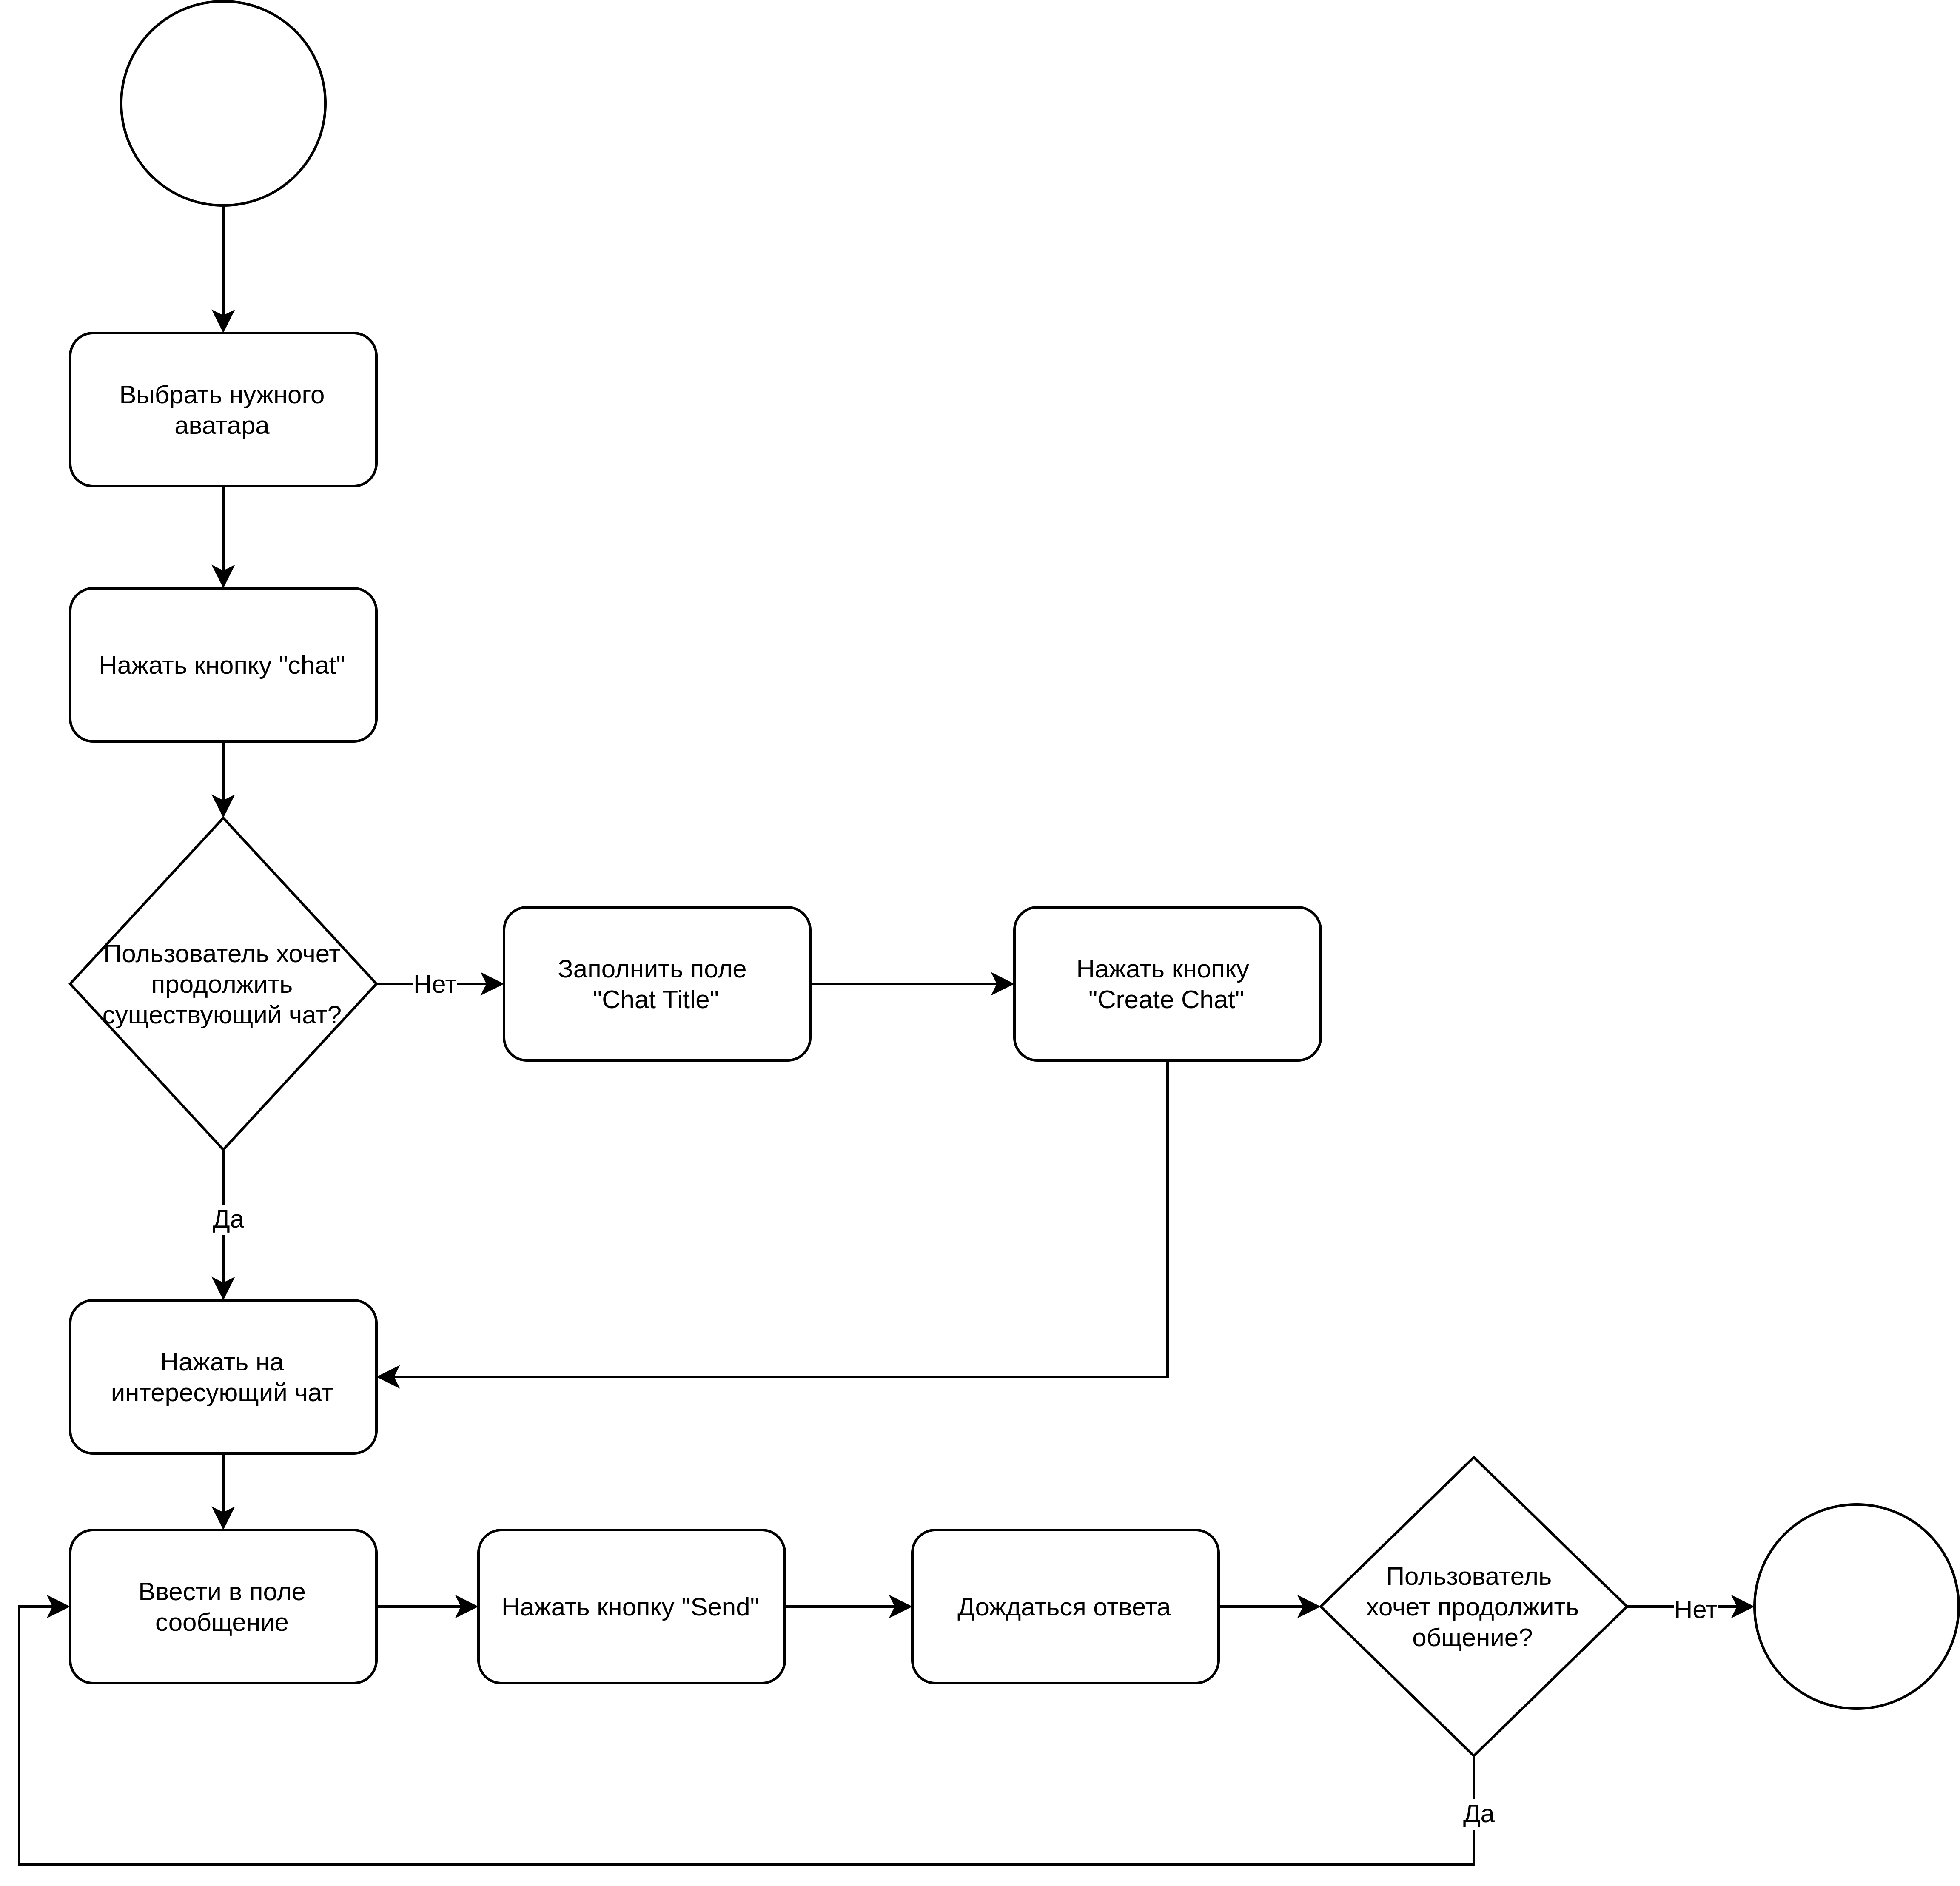
\includegraphics[width=1.0\linewidth]{images/UF-chat-with-avatar.png}
    \caption{User flow диаграмма процесса взаимодействия с аватаром (пользователь уже выполнил вход)}
    \label{fig:uf-chat-with-avatar}
\end{figure}

%FIX ME PLEASE
\begin{figure}
    \centering
    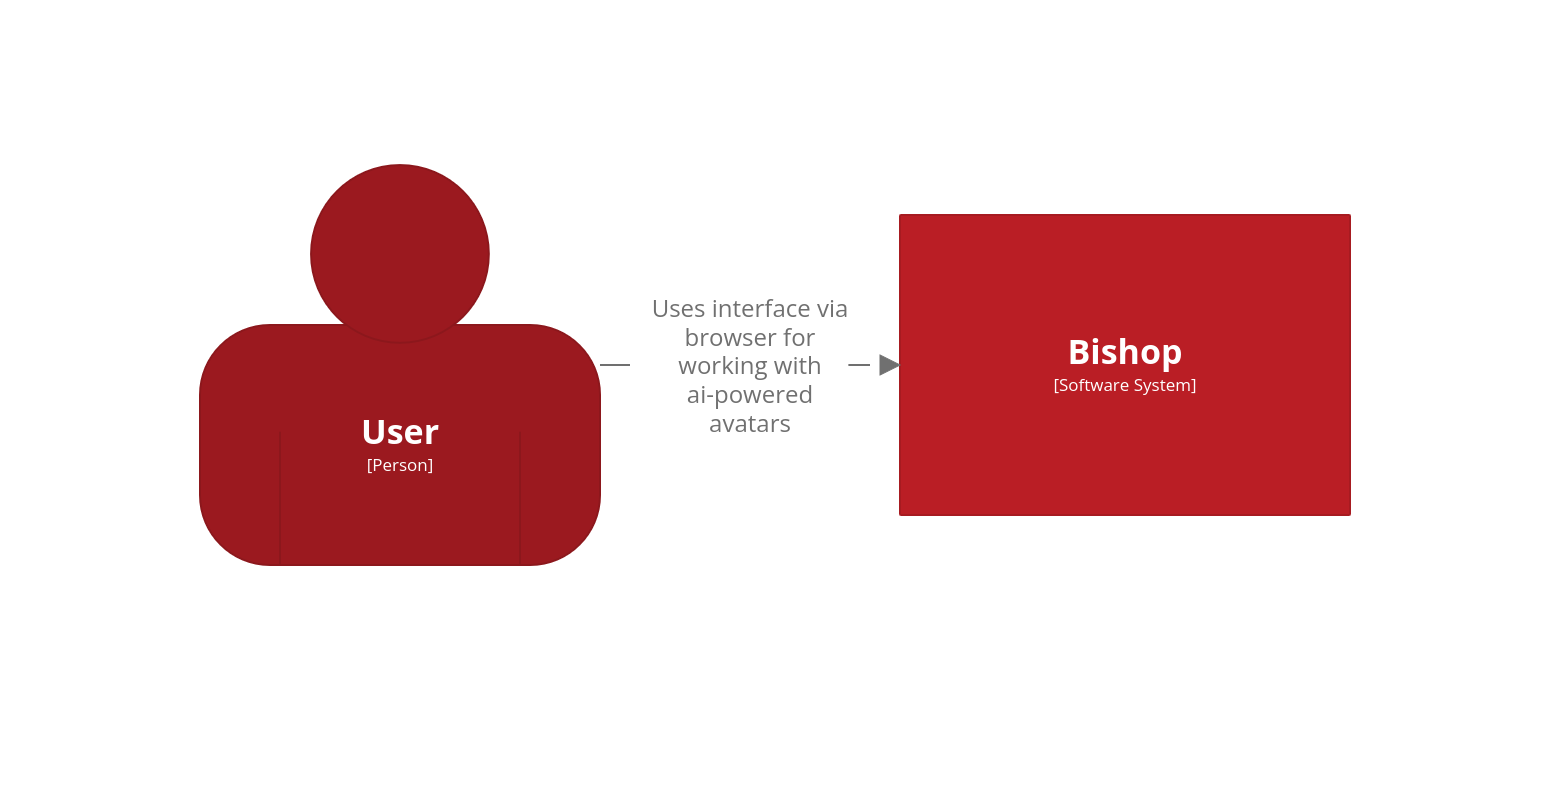
\includegraphics[width=1.0\linewidth]{images/c4-general.png}
    \caption{C4 диаграмма для сервиса <<Bishop>>}
    \label{fig:c4-bishop-1}
\end{figure}

\begin{figure}
    \centering
    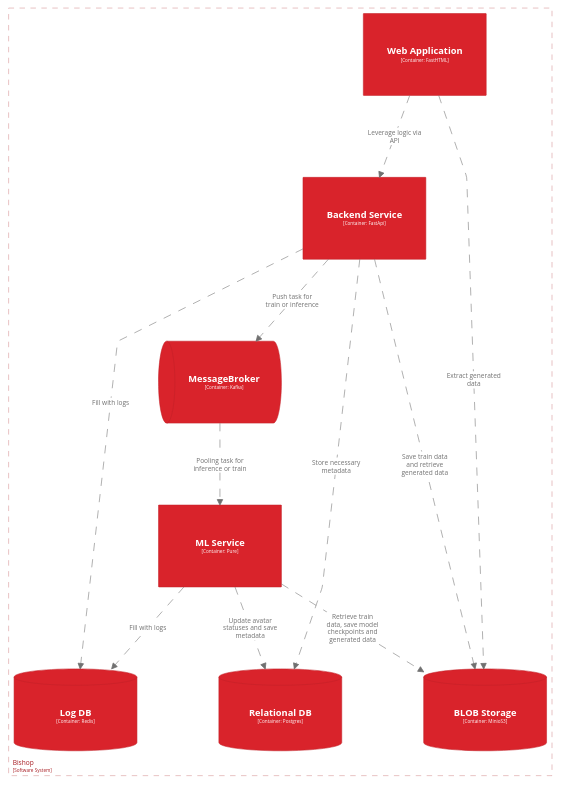
\includegraphics[width=1.0\linewidth]{images/c4-bishop.png}
    \caption{C4 диаграмма для сервиса <<Bishop>>}
    \label{fig:c4-bishop}
\end{figure}

\chapter{Построение модели решения задачи} 
Концепция сервиса опирается на интенсивное использование аппарата машинного обучения. Диаграммы процесса генерации \ref{fig:uml-inference} и обучения \ref{fig:uml-train} дают общее понимание процесса работы данного модуля. Далее будут рассмотрены как теоретические аспекты работы с моделями, так и результаты проведённых экспериментов.

\section{Цели и ограничения}
Основная цель данного модуля заключается в организации эффективного взаимодействия пользователя с аватаром через последовательный обмен сообщениями с последующей озвучкой сгенерированных текстовых сообщений. Ключевой особенностью является реалистичная имитация речевого поведения конкретного человека.

Описанная задача общения аватара с пользователем включает генерацию текста с учётом особенностей личности (persona-based text generation) в контексте домена обработки естественного языка (NLP). Дополнительно решается задача синтеза речи с имитацией голоса реального человека (voice imitation). Также в процессе формирования обучающего корпуса решается вспомогательная задача извлечения текста из аудио- и видеоматериалов (text extraction from audio/video).

Необходимо учитывать, что вычислительные ресурсы для генерации текста и аудио намного меньше, чем ресурсы, необходимые для обучения моделей. В целях демонстрации функционала, общение с аватаром будет осуществляться при помощи заранее обученных моделей, размещённых на бесплатных вычислительных мощностях таких сервисов, как Kaggle и Colab. Для демонстрации процесса обучения будут использованы модели небольших размеров с умеренными параметрами, чтобы снизить нагрузку на вычислительные мощности.


\section{Модуль генерации текста}
\subsection{Данные}
Формирование обучающего корпуса для аватара требует сбора и обработки значительных объёмов данных, характеризующих речевое поведение человека. Корпус включает три основных типа данных: текст, аудио и видео.

Каждый указанный формат поддерживается интерфейсом сервиса с возможностью загрузки популярных расширений файлов. Эти файлы преобразуются в исходные тексты, которые составляют первый тип данных в обучающем корпусе.

Вторым важным источником данных являются социальные сети, представляющие собой естественный источник коммуникации человека в современном мире. Данные социальных сетей имеют структуру вопрос-ответ и требуют персонального согласия пользователя на обработку. Реализована интеграция с мессенджером Telegram для автоматического сбора текстовых, аудио и видеосообщений из выбранных пользователем диалогов.

Итого, обучающий корпус включает исходные тексты, а также диалоговые сообщения из социальных сетей.

После получения данных в пайплайн обучения формируется структурированный датасет для дообучения модели генерации. Видеофайлы конвертируются в аудиофайлы формата WAV с помощью библиотеки moviepy. Затем начинается этап распознавания речи с помощью модели Whisper, аналогичный для полученных аудиофайлов, позволяющий получить текстовую транскрипцию с хорошей точностью.
На следующем шаге преобразованные и полученные текстовые файлы проходят стадию предобработки, в процессе которой удаляются лишние символы, технические вставки. Кроме того, слишком длинные предложения разбиваются на короткие, разбивая в основном на концах предложения, чтобы сохранить читаемость и связность.
В завершение все данные объединяются в единый текстовый корпус, готовый для запуска обучения.


\subsection{Выбор базовой модели}

Выбор языковой модели для задачи генерации текста в речевом стиле конкретного человека основывался на необходимости запуска обучения и генерации на бесплатных вычислительных ресурсах Kaggle, обеспечивая наилучший результат в рамках данных ограничений. Преимуществом использования платформы Kaggle для реализации пайплайнов является предоставление доступа к GPU ресурсам (NVIDIA Tesla P100 или T4), которых, несмотря на ограниченность, вполне достаточно для проведения экспериментов в научном проекте. Также немаловажным фактором в пользу использования данного облачного сервиса стало наличие официального API, который позволяет интегрировать использование вычислительных ресурсов в процесс обучения и генерации. 
На основании анализа научно-технической литературы и сравнительных оценок LLM было принято решение использовать модель из семейства Saiga. Основным критерием выбора послужили высокие результаты в бенчмарке PingPong, ориентированном на оценку в ролевых диалогах, одним из ключевых критериев которых является способность модели сохранять заданную роль. Наличие в обучающих корпусах этой серии данных, которые содержат разнообразные диалоговые и ролевые сценарии, что дополнительно подтверждает пригодность этих моделей для выбранной задачи.
Кроме того, линейка моделей Saiga включает в себя версии различной сложности и размеров, что позволило подобрать оптимальный вариант. Модель saiga\_mistral\_7b\_lora соответствует имеющимся ограничениям по вычислительным ресурсам, обладая хорошим уровнем качества генерации текста.
В рамках ограниченных ресурсов ее применение возможно благодаря технологии QLoRA, при которой модель заранее квантуется до 4-битного представления и фиксирует неизменными часть слоев, что позволяет значительно сократить объем занимаемой памяти при незначительной потере точности. Поэтому ее можно использовать на видеокартах с объёмом памяти 16 ГБ, которые доступны на платформе Kaggle.
Также в описании модели на платформе Hugging Face представлен сравнительный тест, где saiga\_mistral\_7b\_lora показала себя лучше, чем более крупная модель saiga2\_13b\_lora, основанная на архитектуре LLaMA 2, где при тесте 243 ответа были признаны лучшими, против 31 у последней и при 141 ничейном результате. При этом в серии моделей Saiga уступает более новой модели, основанной на архитектуре LLaMA 3, которая требует больших вычислительных ресурсов.


\subsection{Метрики}
На этапе выбора базовой модели для оценки качества генерации текста в речевом стиле конкретного человека главным элементом выступала human evaluation (человеческая экспертиза). Тем не менее учитывались следующие автоматические метрики:
\begin{itemize}
\item Perplexity — стандартная метрика, оценивающая степень «неопределённости» модели в предсказании следующего слова;
\item BLEU (Bilingual Evaluation Understudy) — оценивает сходство сгенерированного текста с эталонными образцами;
\item ROUGE (Recall-Oriented Understudy for Gisting Evaluation) — оценивает качество по наличию ключевых слов и выражений в сгенерированном тексте;
\end{itemize}
Однако численные метрики носили вспомогательный характер, а основное внимание уделялось качественной оценке результатов: насколько текст реалистичен, естественен, и соответствует интонациям и стилевым особенностям пользователя.


\subsection{Токенизация}
Для токенизации текста используется алгоритм Byte-Pair Encoding (BPE), который позволяет эффективно работать с большим словарём слов, сохраняя баланс между объёмом данных и скоростью обработки. Использование BPE помогает эффективно представлять редкие слова и специализированные термины, что особенно важно для персонализированной генерации текста.

\subsection{Обучение}

Процесс дообучения модели реализован в рамках чистой архитектуры, что обеспечило высокую модульность и отделение бизнес-логики от технических деталей. Все ключевые компоненты пайплайна — загрузка данных, проверка ресурсов, запуск обучения и сохранение результатов — организованы в виде изолированных модулей с интерфейсами. Такой подход позволяет быстро адаптировать архитектуру под новые требования в условиях стремительного развития LLM.
Дообучение может запускаться как на локальной машине, так и на бесплатных вычислительных ресурсах Kaggle. Выбор режима настраивается в конфигурационном файле. По умолчанию создается и запускается Kaggle-ноутбук с предварительно загруженным датасетом. Изменением одной переменной можно переключиться на локальное выполнение, что особенно полезно в условиях ограниченного доступа к аппаратным ресурсам.
Запуск пайплайна осуществляется в отдельном процессе, что позволяет оставлять сервис в активном состоянии. Однако новые запросы на обучение игнорируются, пока работает хотя бы одна задача обучения.
Конечная модель сохраняется в S3-хранилище, откуда потом используется для пайплайна генерации текста.

\subsection{Генерация текста}
Генерация текста построена по аналогичной модульной логике: в зависимости от настроек может использоваться локальный или удаленный режим. Ранее дообученная модель загружается из облачного хранилища для генерации ответа. Благодаря изолированной структуре, интеграция новой модели для генерации требует минимальных изменений — достаточно заменить соответствующий компонент, не затрагивая остальную часть пайплайна.
Этот подход сохраняет гибкость системы и упрощает ее масштабирование при работе с различными моделями и окружениями.

\section{Модуль генерации звука}
Для синтеза речи используется короткий аудиофрагмент продолжительностью порядка 15 секунд,  
достаточный для точной имитации тембра и артикуляции голоса пользователя.
Прикладная направленность задача звукового модуля задаёт акцент на практической пригодности решения и рациональном  
использовании вычислительных ресурсов, без разработки принципиально новых архитектур.

\subsection{Выбор базовой модели}

При выборе модели для синтеза речи ключевым критерием была способность точно воспроизводить
голос пользователя на основе короткого аудиофрагмента. В процессе исследования различных
решений, доступных на платформах GitHub и Hugging Face, было рассмотрено несколько подходов.

Одним из первых протестированных решений стала реализация \textbf{Real-Time Voice Cloning}
от CorentinJ \cite{jemine2019voicecloning}. Эта модель демонстрирует хорошие результаты в задачах
клонирования голоса и может работать в реальном времени. Однако, как отмечает сам автор,
существуют более современные и качественные решения в области синтеза речи. В частности,
он рекомендует обратить внимание на проекты, представленные на \textbf{paperswithcode}, а
также на такие решения, как \textbf{CoquiTTS} \cite{coquitts} и \textbf{MetaVoice-1B} \cite{metavoice2024}.

Следует отметить, что, несмотря на то, что проект \textbf{CoquiTTS} более не поддерживается его первоначальной 
командой разработчиков, он продолжает развиваться силами сообщества и остаётся актуальным благодаря регулярным 
обновлениям и исправлениям. В ходе тестирования CoquiTTS продемонстрировал стабильную работу, хорошую адаптацию 
к русскому языку и возможность кастомизации тембра речи, что сделало его оптимальным выбором в качестве 
основной модели синтеза речи в рамках проекта.

Параллельно с этим была предпринята попытка интеграции более актуальной архитектуры \textbf{LLASA} (LLaMA-based Speech Synthesis) \cite{ye2025llasa}. Эти модели представляют собой современные
решения в области синтеза речи, основанные на архитектуре LLaMA и интегрированные с кодеком
XCodec2. Особенностью моделей LLaSA является их способность к высококачественному синтезу речи
и поддержка многозадачного обучения.

Семейство LLaSA включает модели с различным количеством параметров: 1, 3 и 8 миллиардов.
Однако полное переобучение даже минимальной версии \textbf{HKUSTAudio/Llasa-1B} требует
значительных вычислительных ресурсов и большого объёма обучающих данных, что выходит за
рамки доступных возможностей. Поэтому было принято решение использовать предобученную
версию \textbf{Llasa-1B-Multilingual}, обладающую следующими преимуществами:

\begin{itemize}
  \item Высокая естественность синтезируемой речи «из коробки» и унифицированная
        BPE-токенизация без необходимости в G2P-преобразовании.
  \item Компактный объём (около 1 миллиарда параметров), позволяющий проводить тонкую
        настройку модели на одной GPU с объёмом памяти 24 GB.
\end{itemize}

Основным недостатком выбранной модели является отсутствие русского корпуса в изначальной
предобученной выборке, что требует дополнительного дообучения на соответствующих данных.

\subsection{Подготовка данных}

Для обучения и валидации использован открытый корпус  
\textbf{Russian Open Speech To Text}. Из него сформированы  
тематические подкорпуса суммарным объёмом около 460 GB WAV, охватывающие  
бытовую речь, подкасты, лекции, радиопередачи и ролики YouTube. Подготовка  
аудио-текстовых пар включала четыре этапа. Сначала исходные записи проходили  
базовую процедуру нормализацию: обрезку тишины, выравнивание уровня громкости и  
преобразование частоты дискретизации к 16 кГц. Затем текст каждой реплики  
токенизировался встроенной BPE-моделью LLaSA, обеспечивая единый словарь для  
всех языков. Далее аудиодорожки дискретизировались в компактные токены  
кодеком XCodec2. Наконец, пары «текст–звук» сохранялись в формате  
\textbf{Hugging Face Datasets}, что позволяло без дополнительной конвертации  
использовать их в пайплайне дообучения и сохранить больше вычислительных мощностей 
для переобучения модели, а также сохранить целостность сформированных датасетов. 

\begin{table}[h!]
  \centering
  \begin{tabular}{|l|c|c|}
    \hline
    \textbf{Префикс} & \textbf{Объём, GB} \\ 
    \hline
    asr\_calls\_2\_val                       & 2     \\
    buriy\_audiobooks\_2\_val                & 1     \\
    public\_youtube700\_val                  & 2     \\ 
    public\_lecture\_1                       & 0.7   \\
    public\_series\_1                        & 1.9   \\
    asr\_public\_stories\_1                  & 4.1   \\
    asr\_public\_stories\_2                  & 9     \\
    asr\_public\_phone\_calls\_1             & 22.7  \\
    public\_youtube1120\_hq                  & 31    \\
    asr\_public\_phone\_calls\_2             & 66    \\
    public\_youtube700                       & 75    \\
    tts\_russian\_addresses\_rhvoice\_4voices& 80.9  \\
    radio\_2                                 & 154   \\
    public\_youtube1120                      & 237   \\
    \hline
  \end{tabular}
  \caption{Подкорпуса Russian Open Speech To Text, отобранные для дообучения}
  \label{tab:ru_splits}
\end{table}


\subsection{Гиперпараметры дообучения модели}

Для успешного переноса модели на русский язык важное значение имеет выбор гиперпараметров обучения.  
Корректная настройка параметров оптимизации, регуляризации и аппаратного обеспечения обеспечивает  
достижение стабильной сходимости и приемлемого качества генерации. В таблице \ref{tab:ft_hparams}  
приведены ключевые гиперпараметры, использованные в ходе финального цикла дообучения модели.

\begin{table}[h!]
\centering
  \begin{tabular}{|c|c|}
    \hline
    Параметр & Значение \\
    \hline
    Модель & \texttt{HKUSTAudio/Llasa-1B-Multilingual} \\
    \hline
    Тип данных & \texttt{bfloat16}, Flash-Attention 2 \\
    \hline
    Оптимизатор & 8-bit Adam (bitsandbytes) \\
    \hline
    Learning Rate & $5\!\cdot\!10^{-5}$ (cosine schedule) \\
    \hline
    Warmup Ratio & 0.03 \\
    \hline
    Weight Decay & 0.01 \\
    \hline
    Batch Size & 16 аудио-сегментов \\
    \hline
    Эпох & 3 \\
    \hline
    Gradient Acc. & 1 \\
    \hline
    Аппаратная база & одна NVIDIA A100 40 GB \\ 
    \hline
  \end{tabular}
  \caption{Ключевые гиперпараметры дообучения}
  \label{tab:ft_hparams}
\end{table}

\subsection{Процесс дообучения и отслеживание параметров}

Эффективное управление процессом обучения требует постоянного мониторинга показателей, таких как  
функция потерь и другие вспомогательные метрики. Для обеспечения прозрачности экспериментов,  
удобства визуализации динамики и последующего анализа была выбрана платформа Weights \& Biases.  
Данная платформа позволяет фиксировать следующие параметры и характеристики обучения:

\begin{itemize}
  \item графики функции потерь на обучении и валидации;  
  \item изменения значений MOS после завершения дообучения;  
  \item контрольные аудио-сэмплы, позволяющие оценить промежуточные результаты;  
  \item хэш коммита и конфигурацию гиперпараметров для воспроизводимости экспериментов.  
\end{itemize}

На рисунках \ref{fig:loss_curve1} и \ref{fig:loss_curve2} представлены примеры визуализации 
основных параметров, т.е. функции потерь в данном случае, полученные при дообучении модели.

\begin{figure}[h]
  \centering
  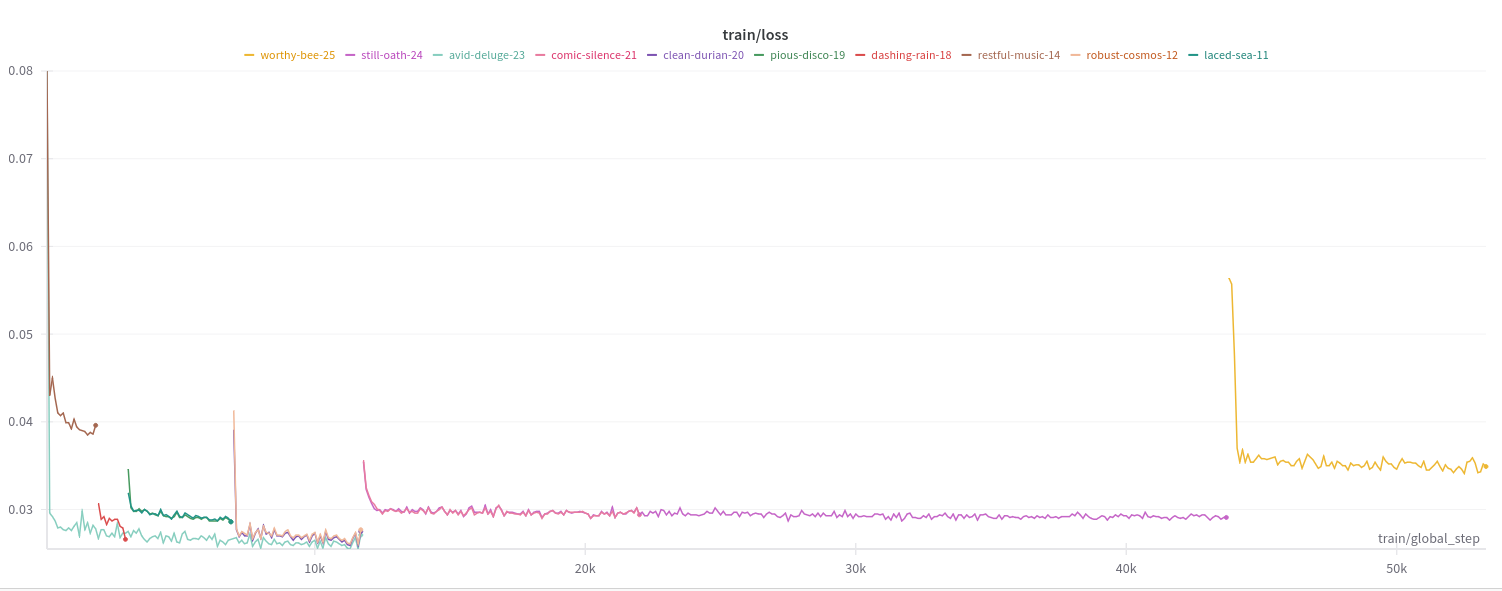
\includegraphics[width=0.9\textwidth]{images/wandb-train-loss.png}
  \caption{Динамика функции потерь на обучении}
  \label{fig:loss_curve1}
\end{figure}

\begin{figure}[h]
  \centering
  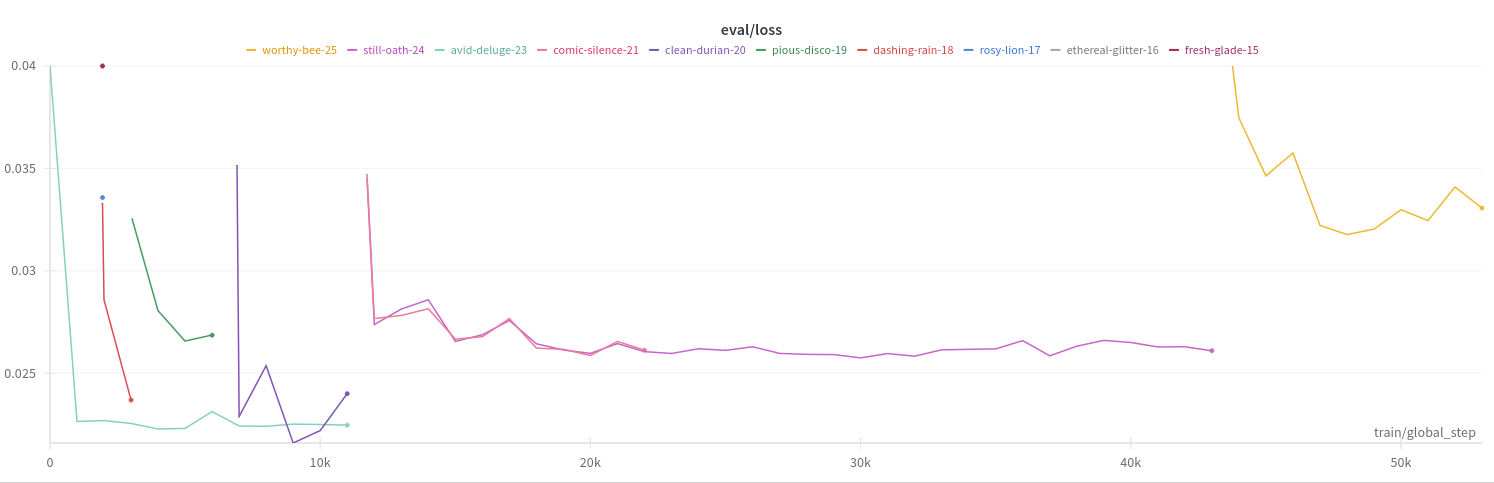
\includegraphics[width=0.9\textwidth]{images/wandb-eval-loss.png}
  \caption{Динамика функции потерь на валидации}
  \label{fig:loss_curve2}
\end{figure}


\subsection{Оценка качества генерации и используемые метрики}

Итоговая оценка качества синтезированной речи представляет собой важнейший этап, подтверждающий практическую пригодность разработанной модели. Особое значение в этом контексте имеет субъективное восприятие конечного пользователя — естественность, эмоциональность и узнаваемость голоса. Для финальной проверки качества планировалось использовать метрику \textbf{Mean Opinion Score (MOS)}, которая широко применяется в задачах оценки качества синтетической речи.

Методика предполагала генерацию набора из 20 «слепых» аудио-сэмплов на фиксированном контрольном тексте, с последующим прослушиванием и оценкой каждого сэмпла группой из пяти независимых слушателей по шкале от 1 до 5. На основе этих оценок рассчитывались среднее значение и дисперсия MOS, что позволило бы количественно зафиксировать степень естественности и узнаваемости полученной речи.

Однако на практике полная реализация данного подхода оказалась невозможной из-за ограниченных вычислительных ресурсов. Провести полноценное обучение модели в запланированном объеме не удалось — была реализована лишь часть обучающих итераций, в результате чего качество сгенерированной речи оставалось далеко от ожидаемого. В таких условиях применение MOS стало неинформативным: оценки слушателей варьировались случайным образом, не отражая объективных различий в качестве, а результирующие значения средней оценки не позволяли сделать достоверные выводы. Таким образом, при текущем уровне реализации метрика MOS оказалась неприменимой и не может использоваться для формальной оценки итогового качества.

В связи с вышеописанными ограничениями, для получения качественных аудио-сэмплов было принято решение использовать готовую модель из библиотеки \textbf{Coqui TTS}.

\chapter{Программная реализация}

\section{Веб-интерфейс}
Веб-интерфейс является важнейшим элементом пользовательского взаимодействия с системой, обеспечивая доступ ко всему спектру функциональных возможностей приложения Bishop.
В данной главе будет рассмотрена структура интерфейса, описаны отдельные страницы и реализуемые ими задачи, а также представлен детальный анализ технических решений,
используемых при разработке.

\subsection{Гостевая страница}
Первая страница веб-интерфейса, доступная пользователю, представляет собой гостевую посадочную страницу \ref{fig:ui-page-welcome} (landing page). Она разработана с целью ознакомления пользователей с проектом Bishop и не требует предварительной авторизации.


Страница выполнена в минималистичном стиле, что позволяет сфокусировать внимание пользователя на основном содержании. В верхней части расположено название проекта «Bishop Ai Application», а справа в шапке страницы находятся две активные ссылки: «Login» и «Signup», позволяющие перейти к авторизации или регистрации соответственно.


Центральная часть страницы содержит краткое приветствие пользователя («Welcome to BishopApp») и детальное описание основной идеи и функционала приложения. 


Нижний колонтитул страницы содержит информацию об авторских правах, что завершает композицию интерфейса и подчеркивает официальность ресурса.

\subsection{Идентификация, аутентификация и авторизация}

Сервис Bishop предусматривает возможность идентификации и авторизации пользователей через формы 
входа \ref{fig:ui-page-login} («Login») и регистрации \ref{fig:ui-page-signup} («Signup»).

Страница входа содержит поля для ввода электронной почты и пароля. После отправки данных 
производится запрос к backend API, который проверяет подлинность введенных данных. В случае 
успешного входа система переадресует пользователя на личную страницу, при этом отображая 
уведомление с текстом «login is successful!». Если данные введены неверно, интерфейс 
отображает сообщение об ошибке («Incorrect email or password»), что существенно улучшает 
пользовательский опыт, четко информируя о причинах невозможности авторизации.

\subsubsection{Регистрация}

Форма регистрации аналогична форме входа, однако требует от пользователя дополнительной информации 
в виде полного имени. Введенные данные валидируются как на уровне фронтенда (проверка 
формата email и минимальной длины пароля), так и на стороне бэкенда (проверка уникальности email). 
Ошибки ввода или проверки также сопровождаются информативными уведомлениями:

\begin{itemize}
  \item \texttt{value is not a valid email address} — если указан некорректный адрес электронной почты.
  \item \texttt{String should have at least 8 characters} — при слишком коротком пароле.
  \item \texttt{The user with this email already exists in the system} — если email уже зарегистрирован.
\end{itemize}

\subsubsection{Техническая реализация и безопасность данных}

Для реализации процесса авторизации используется стандарт JWT. После успешной 
аутентификации токен сохраняется в сессии пользователя и добавляется в заголовки каждого запроса 
к backend API, что обеспечивает надежную защиту и конфиденциальность данных пользователя:

\begin{lstlisting}[language=Python, numbers=none, frame=none]
def get_auth_headers(sess):
    jwt_keys = ["token_type", "access_token"]
    for key in jwt_keys:
        if key not in sess:
            return None

    token_type = sess["token_type"]
    token = sess["access_token"]
    headers = {"Authorization": f"{token_type} {token}"}

    return headers
\end{lstlisting}

Дополнительным слоем безопасности является проверка действительности JWT-токена при каждой попытке 
доступа к защищённым страницам посредством специального промежуточного обработчика 
jwt\_before:

\begin{lstlisting}[language=Python, numbers=none, frame=none]
async def jwt_before(req, sess):
    jwt_keys = ["token_type", "access_token"]
    for key in jwt_keys:
        if key not in sess:
            return Redirect("/")

    auth_hdrs = {"Authorization": f"{sess['token_type']} {sess['access_token']}"}

    async with httpx.AsyncClient(headers=auth_hdrs) as cli:
        res = await cli.post(BACKEND_URL + "/login/test-token")

    if res.status_code != 200:
        return Redirect("/")
\end{lstlisting}

Данные подходы позволяют обеспечить высокую степень защиты персональных данных и контролируемость 
доступа к ресурсам приложения.

\subsection{Основная страница приложения}

После успешной авторизации пользователь перенаправляется на главную страницу \ref{fig:ui-page-index}, являющуюся единственной страницей в архитектуре SPA. Все дальнейшие действия 
пользователя инициируют частичное обновление элементов DOM, не приводя к полной перезагрузке 
страницы. Такой подход значительно повышает отзывчивость и удобство использования приложения.


Главная страница состоит из следующих элементов:
\begin{itemize}
    \item Информация о пользователе
    \item Функциональные элементы для менеджмента аватаров
\end{itemize}


В верхней части страницы располагается блок с персональными данными авторизованного пользователя, 
включающий его имя и адрес электронной почты, а также кнопку выхода («Sign Out») для завершения 
текущей сессии.


Ниже блока с информацией пользователя находится основной функционал, предназначенный для работы с 
цифровыми аватарами:

\begin{itemize}
  \item \textbf{Создание аватара:} Пользователь вводит имя нового аватара в соответствующее 
        текстовое поле и нажимает кнопку \texttt{Create Avatar}. После успешного создания 
        аватара выводится уведомление (\texttt{Avatar created successfully!}) в виде 
        toast-сообщения.
  \item \textbf{Список аватаров:} Все созданные пользователем аватары отображаются в виде 
        кнопок, расположенных в специальном блоке. По клику на аватар открываются дополнительные 
        элементы управления (редактирование, удаление, чат и обучение), при этом не происходит 
        полной перезагрузки страницы.
\end{itemize}


Технически реализация создания аватара представлена следующим образом:

\begin{lstlisting}[language=Python, numbers=none, frame=none]
@dataclass
class AvatarCreateInfo:
    name: str

@rt("/avatar-create")
async def avatar_create(avatar_info: AvatarCreateInfo, sess):
    async with httpx.AsyncClient(headers=get_auth_headers(sess)) as cli:
        res = await cli.post(
            f"{BACKEND_URL}/avatars/", 
            json=asdict(avatar_info)
        )

        if res.status_code == 200:
            add_toast(sess, "Avatar created successfully!", "info")
            return Redirect("/index")
\end{lstlisting}


Использование асинхронных запросов (\texttt{httpx.AsyncClient}) и JWT-токенов в заголовках запроса 
гарантирует безопасность операций и соответствие высоким стандартам защиты пользовательских данных.

\subsection{Страница работы с аватаром}
Страница работы с конкретным аватаром \ref{fig:ui-page-avatar} представляет собой ключевую часть веб-интерфейса Bishop, 
позволяющую получить доступ ко всему основному функционалу, связанному с взаимодействием и 
управлением аватаром. Эта страница является динамически загружаемым компонентом основного 
SPA-приложения и отображается при выборе конкретного аватара из списка.


На странице представлена карточка с именем аватара и набор кнопок, каждая из которых предоставляет 
доступ к определенному функционалу:

\begin{itemize}
  \item \textbf{Train} — переход к интерфейсу загрузки новых материалов для обучения модели аватара 
        и управления процессом её обучения.
  \item \textbf{Chat} — переход к разделу общения с аватаром, где пользователь может взаимодействовать 
        с виртуальной персоной в режиме диалога.
  \item \textbf{Change Name} — позволяет изменить имя выбранного аватара через простой и удобный интерфейс.
  \item \textbf{Delete} — реализует удаление аватара, сопровождаемое подтверждением действия со стороны 
        пользователя, что предотвращает случайные ошибки.
  \item \textbf{To avatars list} — возвращает пользователя обратно к общему списку аватаров.
\end{itemize}


CRUD-функционал реализован асинхронными вызовами к backend API, 
что повышает скорость взаимодействия и удобство использования приложения.


Пример кода реализации переименования аватара:

\begin{lstlisting}[language=Python, numbers=none, frame=none]
@rt("/avatar/{avatar_id}/change_name", methods=["POST"])
async def change_name(avatar_id: str, name: str, sess):
    async with httpx.AsyncClient(headers=get_auth_headers(sess)) as client:
        response = await client.put(
            f"{BACKEND_URL}/avatars/{avatar_id}",
            json={"name": name}
        )
    if response.status_code == 200:
        add_toast(sess, "Avatar renamed successfully!", "success")
    else:
        add_toast(sess, "Failed to rename avatar.", "error")

    return Redirect(f"/index")
\end{lstlisting}


Пример кода реализации удаления аватара:

\begin{lstlisting}[language=Python, numbers=none, frame=none]
@rt("/avatar/{avatar_id}/delete", methods=["POST"])
async def delete_avatar(avatar_id: str, sess):
    async with httpx.AsyncClient(headers=get_auth_headers(sess)) as client:
        response = await client.delete(
            f"{BACKEND_URL}/avatars/{avatar_id}"
        )

    if response.status_code == 200:
        add_toast(sess, "Avatar deleted!", "success")
    else:
        add_toast(sess, "Failed to delete avatar.", "error")

    return Redirect("/index")
\end{lstlisting}


Взаимодействие с backend происходит через запросы с авторизационными JWT-токенами, что гарантирует 
сохранность и защищенность данных пользователя.

\subsection{Интерфейс общения с аватаром}

Один из центральных элементов веб-интерфейса — это возможность вести живой диалог с 
цифровым аватаром. Для реализации этого функционала предусмотрен отдельный интерфейс чата \ref{fig:ui-page-chat2}. 
Пользователь может создать несколько отдельных чатов для каждого аватара на отдельно странице для 
менеджмента чатов \ref{fig:ui-page-chat1}, например, на различные 
темы. Каждый чат имеет своё название, задаваемое пользователем при его создании.


После выбора чата пользователю открывается интерфейс переписки, состоящий из:

\begin{itemize}
  \item поля для ввода текста сообщения;
  \item кнопки отправки сообщения (\texttt{Send});
  \item кнопки возврата к списку чатов (\texttt{Back to Chats}).
\end{itemize}


Особенностью взаимодействия является то, что аватар не только генерирует текстовые ответы, но и 
озвучивает их. После отправки сообщения пользователь видит свой вопрос и автоматически 
отображающееся сообщение о том, что аватар формирует ответ (\texttt{Avatar is typing...}).


Как только модель сформирует ответ, сообщение заменяется текстовым ответом аватара и 
аудиопроигрывателем, позволяющим прослушать ответ. Это обеспечивает эффект живого диалога и 
существенно улучшает восприятие взаимодействия.


Для реализации подобного поведения использованы асинхронные запросы с механизмом 
polling-запросов (периодические запросы к backend API для получения статуса готовности ответа):

\begin{lstlisting}[language=Python, numbers=none, frame=none]
@rt("/avatar/{avatar_id}/chat/{chat_id}/poll_response/{rsp_msg_id}/")
async def poll_response(avatar_id: str, chat_id: str, rsp_msg_id: str, sess):
    async with httpx.AsyncClient(headers=get_auth_headers(sess)) as client:
        for _ in range(3):
            await asyncio.sleep(2)

            msg_url = (
                f"{BACKEND_URL}/avatars/{avatar_id}/chat/{chat_id}"
                f"/msgs/{rsp_msg_id}/response/"
            )
            res = await client.get(msg_url)
            if res.status_code != 200:
                continue

            msg = res.json()
            audio_url = (
                f"{BACKEND_URL}/avatars/{avatar_id}/chat/{chat_id}"
                f"/msgs/{rsp_msg_id}/response/dub/"
            )
            audio_res = await client.get(audio_url)

            if audio_res.status_code == 200:
                b64 = base64.b64encode(audio_res.content).decode("ascii")
                return Div(
                    P(f"Avatar: {msg['text']}"),
                    Audio(
                        controls=True,
                        autoplay=False,
                        preload="auto",
                        src=f"data:audio/x-wav;base64,{b64}"
                    ),
                    cls="chat-message-bot"
                )
\end{lstlisting}


Таким образом, интерфейс обеспечивает интерактивное взаимодействие с аватаром, совмещая текстовую 
переписку с живым голосовым сопровождением, что делает диалог максимально близким к естественной 
коммуникации.

\subsection{Интерфейс обучения аватара}
Также ключевым элементом функционала является раздел обучения аватара \ref{fig:ui-page-train}. Пользователю 
доступен расширенный набор действий, позволяющий совершенствовать аватар посредством добавления новых 
обучающих материалов и управления процессом обучения.


На странице обучения пользователь может загрузить материалы двух основных типов:
\begin{itemize}
  \item \textbf{Аудио для синтеза голоса:} Короткие аудио-файлы формата \texttt{.wav}, используемые 
        для создания реалистичной модели голоса аватара.
  \item \textbf{Материалы для извлечения текста:} Аудио, видео или текстовые документы, из которых 
        будет извлечён текстовый контент для обучения языковой модели аватара.
\end{itemize}


Пользовательский интерфейс загрузки материалов представлен формой с возможностью выбора типа 
материалов и загрузки нескольких файлов одновременно:

\begin{itemize}
  \item Выпадающий список выбора типа загружаемых данных (\texttt{Extract text} или 
        \texttt{Voice synthesis}).
  \item Поле выбора файлов и кнопка загрузки.
\end{itemize}


После загрузки файлы отображаются в списке текущих материалов для обучения, где для каждого файла 
указывается тип и ссылка для скачивания.


Пример реализации загрузки материалов на уровне frontend:

\begin{lstlisting}[language=Python, numbers=none, frame=none]
@rt("/avatar/{avatar_id}/train", methods=["POST"])
async def proxy_upload(avatar_id: str, request: Request, sess):
    form = await request.form()
    uploaded_files = form.getlist("files")
    type_value = form.get("type")

    file_data = []
    for file in uploaded_files:
        content = await file.read()
        file_data.append((
            "file", 
            (file.filename, content, file.content_type)
        ))

    async with httpx.AsyncClient(headers=get_auth_headers(sess)) as client:
        res = await client.post(
            f"{BACKEND_URL}/avatars/{avatar_id}/train/",
            data={"type": type_value},
            files=file_data
        )

    if res.status_code == 200:
        add_toast(sess, "File uploaded successfully!", "info")
    else:
        add_toast(sess, "File upload failed!", "error")

    return await avatar_train_widget(avatar_id, sess)
\end{lstlisting}


Пользователь может непосредственно управлять процессом обучения, используя две основные кнопки:

\begin{itemize}
  \item \textbf{Start Training:} Инициирует процесс обучения модели аватара с использованием всех 
        загруженных материалов. После старта обучения статус модели изменяется на 
        \texttt{training}.
  \item \textbf{Stop Training:} Позволяет принудительно остановить процесс обучения. После 
        остановки статус модели меняется обратно на \texttt{available}, и пользователю вновь 
        предоставляется возможность запуска нового обучения.
\end{itemize}


Реализация управления статусом обучения:

\begin{lstlisting}[language=Python, numbers=none, frame=none]
@rt("/avatar/{avatar_id}/train/start", methods=["POST"])
async def avatar_train_start(avatar_id: str, sess):
    async with httpx.AsyncClient(headers=get_auth_headers(sess)) as client:
        await client.post(
            f"{BACKEND_URL}/avatars/{avatar_id}/train/start"
        )

    return await avatar_train_widget(avatar_id, sess)


@rt("/avatar/{avatar_id}/train/stop", methods=["POST"])
async def avatar_train_stop(avatar_id: str, sess):
    async with httpx.AsyncClient(headers=get_auth_headers(sess)) as client:
        await client.post(
            f"{BACKEND_URL}/avatars/{avatar_id}/train/stop"
        )

    return await avatar_train_widget(avatar_id, sess)
\end{lstlisting}


Интерфейс динамически отражает текущее состояние аватара, показывая статус модели (\texttt{training}, 
\texttt{available}), список загруженных материалов и соответствующие уведомления, обеспечивая 
высокий уровень прозрачности и удобства для пользователя.


Таким образом, Bishop предоставляет удобный и интуитивно понятный интерфейс для полноценного управления 
обучением аватаров, поддерживая оперативный контроль за текущим состоянием и эффективное взаимодействие 
с системой.

\section{Backend-сервис}
Backend-сервис является центральным узлом системы, обеспечивающим взаимодействие между всеми ключевыми компонентами:
\begin{itemize}
    \item Веб-интерфейс
    \item База данных
    \item ML-сервис
    \item S3-хранилище
\end{itemize}

В следующих разделах мы подробно разберем ключевые особенности имплементации, связанные с взаимодействием backend-сервиса с каждым конкретным узлом системы.

\subsection{Взаимодействие с веб-интерфейсом}
Ключевой библиотекой, которая используется в backend-сервисе для работы с веб-интерфейсом является FastApi, которая позволяет быстро и эффективно описывать структурированный API, поддерживает асинхронный режим работы, а так же автоматически генерирует документацию через OpenApi(Swagger).

\subsubsection{Группировка HTTP методов и соответствующих модулей}
При проектировании API использовался устоявшийся в индустрии метод, согласно которому маршруты разделялись по HTTP-методам. Такой метод позволяет упростить и стандартизировать взаимодействие между backend-сервисом и веб-интерфейсом. Так же это может упростить и сделать API понятным для сторонних разработчиков.

Для удобства и простоты поддержки маршруты дополнительно были сгруппированы в отдельные модули:
\begin{itemize}
    \item users - управление пользователями
    \item train – загрузка данных для обучения
    \item msgs – управление сообщениями
    \item chats – управление чатами
    \item avatars – управление аватарами
\end{itemize}

Ниже приведены примеры маршрутов, используемые для создания ресурсов и их краткое описание:

\begin{itemize}
    \item \texttt{POST /api/v1/avatars} – тело запроса состоит из json-объекта, единственным полем которого является строка. Строка передает в систему имя аватара, которого хочет создать пользователь.\newline
    Структура json-объекта:
    \begin{lstlisting}[style=jsonstyle, numbers=none, frame=none]
    {
       "name": "Avatar's name"
    }
    \end{lstlisting}
    
    \item \texttt{POST /api/v1/avatars/\{avatar\_id\}/chat} – тело запроса вновь состоит из строки, которая несет в себе имя для чата, который хочет создать пользователь. В отличие от первого примера URI содержит в себе параметр \texttt{\{avatar\_id\}}, отвечающий за идентификацию конкретного аватара пользователя.\newline
    Структура json-объекта:
    \begin{lstlisting}[style=jsonstyle, numbers=none, frame=none]
    {
       "title": "Chat's title"
    }
    \end{lstlisting}

    \item \texttt{POST /api/v1/avatars/\{avatar\_id\}/chat/\{chat\_id\}/msgs} – несет в себе полезную нагрузку в виде строки, которую набрал пользователь при отправке очередного сообщения. URI содержит \texttt{\{avatar\_id\}} и \texttt{\{chat\_id\}}.\newline
    Структура json-объекта:
    \begin{lstlisting}[style=jsonstyle, numbers=none, frame=none]
    {
       "message": "User's message"
    }
    \end{lstlisting}

    \item \texttt{POST /api/v1/users} – содержит json объект с полями email, isSuperuser, isActive, fullName, password. Все эти поля используются для создания записи о пользователе в базе данных.\newline
    Структура json-объекта:
    \begin{lstlisting}[style=jsonstyle, numbers=none, frame=none]
    {
       "email": "user@example.com",
       "isSuperuser": false,
       "isActive": true,
       "fullName": "User's fullname",
       "password": "secret"
    }
    \end{lstlisting}

    \item \texttt{POST /api/v1/avatars/\{avatar\_id\}/train} – в теле запроса несет бинарное представление файла пользователя и его метаданные такие как имя файла и формат. URI содержит \texttt{\{avatar\_id\}}.
\end{itemize}

\subsubsection{Пример описания обработчика из модуля users}
Ниже приведен пример исходного кода функции, которая занимается обработкой запросов на создание нового пользователя:
\begin{lstlisting}[language=Python, numbers=none, frame=none]
@router.post(
    "/",
    dependencies=[Depends(get_current_active_superuser)],
    response_model=UserPublic
)
async def create_user(
        *,
        session: SessionDep,
        user_in: UserCreate
) -> User:
    """
    Create new user.
    """
    user = await user_repository.get_user_by_email(session=session, email=user_in.email)
    if user:
        raise HTTPException(
            status_code=400,
            detail="The user with this email already exists in the system.",
        )

    user = await user_repository.create_user(session=session, user_create=user_in)

    if settings.emails_enabled and user_in.email:
        email_data = generate_new_account_email(
            email_to=user_in.email, username=user_in.email, password=user_in.password
        )
        send_email(
            email_to=user_in.email,
            subject=email_data.subject,
            html_content=email_data.html_content,
        )
    return user
\end{lstlisting}
Представленный код демонстрирует общий подход к написанию обработчиков в backend-сервисе.\newline
Ключевые архитектурные элементы:
\begin{itemize}
    \item Pydantic-модели - обеспечивают строгую типизацию и автоматическую валидацию
    \item Система зависимостей (Depends) - инкапсулируют повторяющуюся логику
    \item Разделение ответственности - для работы с БД и другими сущностями обработчики вызывают функции из отдельных модулей
    \item Декораторы - стандартизируют HTTP-метод, путь и формат ответа
    \item Обработка ошибок - единый стиль обработки через HTTPException
\end{itemize}

\subsection{Взаимодействие с базой данных}

\subsubsection{Основные сведения о реализации}
В backend сервисе для работы с базой данных используется библиотека SQLModel. В исходном коде сервиса активно используются следующие преимущества этой библиотеки:
\begin{itemize}
  \item Работа с записями БД как с объектами Python
  \item Встроенная валидация данных на основе аннотаций типов
  \item Поддержка асинхронных операций.
\end{itemize}

Все сущности, которые семантически относятся к записям в базе данных или содержат в себе информацию, которая должна попасть в базу данных были описаны с помощью специальных классов, которые в данном контексте принято называть моделями.
Эти модели можно разделить на два типа:
\begin{itemize}
    \item Модели БД – описывают структуру таблиц в базе данных
    \item Pydantic-модели (прокси-классы), которые используются для:
    \begin{itemize}
        \item Валидации входящих json-данных
        \item Сериализации ответов API
        \item Предварительной обработки данных
    \end{itemize}
\end{itemize}

\subsubsection{Пример реализации}
Рассмотрим на примере сущности User организацию моделей для обработки запросов и работы с БД:
\begin{lstlisting}[language=Python, numbers=none, frame=none]
class UserBase(SQLModel):
   email: EmailStr = Field(unique=True, index=True, max_length=255)
   is_active: bool = True
   is_superuser: bool = False
   full_name: str | None = Field(default=None, max_length=255)


class UserCreate(UserBase):
   password: str = Field(min_length=8, max_length=40)


class User(UserBase, table=True):
   __tablename__ = "user"
   id: uuid.UUID = Field(default_factory=uuid.uuid4, primary_key=True)
   hashed_password: str
   avatars: list["Avatar"] = Relationship(
       back_populates="user", cascade_delete=True)
\end{lstlisting}

Модели организованы по принципу наследования:
\begin{itemize}
    \item UserBase - базовый класс, содержащий общие поля, которые присутствуют во всех производных моделях. Служит для избежания дублирования кода.
    \item UserCreate - модель для валидации входящих данных при создании пользователя. Если json-объект в теле запроса не соответствует этой модели, сервер автоматически возвращает ошибку 422 Unprocessable Entity с детальным описанием проблем валидации, что избавляет разработчика от необходимости писать рутинный код для проверки входных данных.
    \item User - основная модель, которая описывает структуру таблицы БД, наследует все функциональные возможности SQLAlchemy и используется для непосредственных запросов к БД
\end{itemize}

Рассмотрим преимущества такой структуры кода на примере, когда API получает запрос на создание нового пользователя и вызывает функцию, которая инкапсулирует в себе обращение к БД для создания новой записи:
\begin{lstlisting}[language=Python, numbers=none, frame=none]
async def create_user(*, session: AsyncSession, user_create: UserCreate) -> User:
   db_obj = User.model_validate(
       user_create, update={
           "hashed_password": get_password_hash(user_create.password)}
   )
   session.add(db_obj)
   await session.commit()
   await session.refresh(db_obj)
   return db_obj
\end{lstlisting}
В этом примере стоит обратить внимание на следующие пункты, которые раскрывают удобство описываемого подхода:
\begin{itemize}
    \item Входящие данные автоматически валидируются моделью UserCreate
    \item Готовый объект User сохраняется в БД
    \item Происходит преобразование UserCreate → User с:
    \begin{itemize}
        \item Автоматическим заполнением недостающих полей
        \item Игнорированием нерелевантных данных
    \end{itemize}
\end{itemize}

\subsubsection{Структура модулей для работы с разными таблицами в БД}
Для каждой сущности из базы данных (рис. \ref{fig:db_structure}) реализован отдельный модуль, содержащий:
\begin{itemize}
    \item CRUD-операции – базовые создание, чтение, обновление и удаление записей
    \item Специфическую логику – например, загрузка бинарных данных для обучения в S3 хранилище, с последующим сохранением URL в базу данных
\end{itemize}

Такое архитектурное решение предоставляет ряд преимуществ:
\begin{itemize}
    \item Четкое разделение ответственности – каждый модуль отвечает только за свою сущность
    \item Масштабируемость – добавление новых сущностей не ломает существующий код
    \item Упрощение поддержки – изменения в одной сущности не затрагивают другие
    \item Удобство тестирования – модули можно проверять изолированно
\end{itemize}


На примере модуля, отвечающего за операции с пользователями, рассмотрим стандартные CRUD-функции и их назначение:

\begin{itemize}
    \item Получение списка пользователей
    \begin{lstlisting}[language=Python, numbers=none, frame=none]
    async def get_users(*, session: AsyncSession, skip: int = 0, limit: int = 100) -> list[User]:
    \end{lstlisting}
    
    \item Создание пользователя
    \begin{lstlisting}[language=Python, numbers=none, frame=none]
    async def create_user(*, session: AsyncSession, user_create: UserCreate) -> User:
    \end{lstlisting}

    \item Обновление пользователя
    \begin{lstlisting}[language=Python, numbers=none, frame=none]
    async def update_user(*, session: AsyncSession, db_user: User, user_in: UserUpdate) -> Any:
    \end{lstlisting}

    \item Поиск пользователя по email
    \begin{lstlisting}[language=Python, numbers=none, frame=none]
    async def get_user_by_email(*, session: AsyncSession, email: str) -> User | None:
    \end{lstlisting}

    \item Аутентификация пользователя
    \begin{lstlisting}[language=Python, numbers=none, frame=none]
    async def authenticate(*, session: AsyncSession, email: str, password: str) -> User | None:
    \end{lstlisting}
\end{itemize}

На данном примере можно отметить ряд особенностей, которые выполняются для всех подобных модулей:
\begin{itemize}
    \item Типизация - все функции строго типизированы
    \item Единообразный подход в формировании сигнатур
    \item Соответствие названий функций семантике
\end{itemize}




 \begin{figure}[h!]
     \centering
     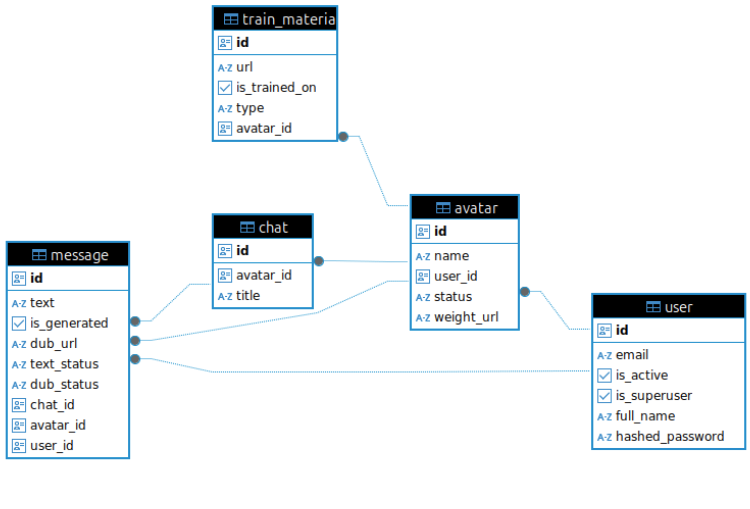
\includegraphics[width=1.0\linewidth]{images/db_structure.png}
     \caption{Структура базы данных}
     \label{fig:db_structure}
 \end{figure}



\subsection{Взаимодействие с ML-сервисом}
Взаимодействие backend с ML-сервисом осуществляется через брокер сообщений Kafka. Для работы с брокером используется библиотека aiokafka.

Чтобы обеспечить удобство поддержки и разделение ответственности, логика работы с брокером была инкапсулирована в две отдельные сущности. Критерием разделения стало направление сообщений:
\begin{itemize}
    \item KafkaMessageProducer — отвечает за формирование и отправку сообщений в ML-сервис
    \item MessageManagerConsumer — обрабатывает входящие сообщения от ML-сервиса
\end{itemize}

Такое разделение позволяет упростить масштабирование, тестирование и модификацию каждого компонента в будущем, а также не накладывает ограничений на возможность параллельной разработки.


\subsubsection{Формирование и передача запросов к ML-сервису}
KafkaMessageProducer представляет собой клиентский модуль, отвечающий за отправку заранее сформированных сообщений в Kafka. Для каждого типа сообщения реализована отдельная функция, которая использует интерфейс клиента для передачи данных в брокер.\newline
Типы сообщений:
\begin{itemize}
    \item \texttt{start\_train} — запускает обучение аватара
    \item \texttt{stop\_train} — останавливает процесс обучения;
    \item \texttt{inference\_response} — инициирует генерацию текстового ответа на сообщение пользователя;
    \item \texttt{sound\_inference} — запускает синтез озвучки для сгенерированного текста.
\end{itemize}

1. Сообщение \texttt{start\_train}
\begin{lstlisting}[style=jsonstyle, numbers=none, frame=none]
{
   "event": "train_start",
   "avatar_id": avatar_id,
   "train_materials": [
      {
         "id": material.id,
         "type": material.type,
         "url": material.url
      }
   ]
}
\end{lstlisting}
Описание полей:
\begin{itemize}
    \item \texttt{event} - тип события
    \item \texttt{avatar\_id} - уникальный идентификатор аватара
    \item \texttt{train\_materials} - список объектов для обучения:
    \begin{itemize}
        \item \texttt{id} - уникальный идентификатор материала
        \item \texttt{type} - тип материала
        \item \texttt{url} - путь в S3
    \end{itemize}
\end{itemize}

2. Сообщение \texttt{stop\_train}
\begin{lstlisting}[style=jsonstyle, numbers=none, frame=none]
{
   "event": "train_stop",
   "avatar_id": avatar_id
}
\end{lstlisting}
Описание полей:
\begin{itemize}
    \item \texttt{event} - тип события
    \item \texttt{avatar\_id} - уникальный идентификатор аватара
\end{itemize}

3. Сообщение \texttt{inference\_response}
\begin{lstlisting}[style=jsonstyle, numbers=none, frame=none]
{
   "event": "inference_response",
   "message_id": message_id,
   "text": user_message
}
\end{lstlisting}
Описание полей:
\begin{itemize}
    \item \texttt{event} - тип события
    \item \texttt{message\_id} - уникальный идентификатор сообщения пользователя
    \item \texttt{text} - текст сообщения пользователя
\end{itemize}

3. Сообщение \texttt{sound\_inference}
\begin{lstlisting}[style=jsonstyle, numbers=none, frame=none]
{
    "event": "sound_inference",
    "storage_url": storage_url,
    "base_voice_url": base_voice_url,
    "message_id": message_id,
    "text": gen_message,
}
\end{lstlisting}
Описание полей:
\begin{itemize}
    \item \texttt{event} - тип события
    \item \texttt{storage\_url} - путь в S3, где нужно будет сохранить результат
    \item \texttt{base\_voice\_url} - путь в S3, откуда брать голос для озвучки
    \item \texttt{message\_id} - уникальный идентификатор сообщения, для которого требуется озвучка
    \item \texttt{text} - текст сообщения, которое нужно озвучить
\end{itemize}

\subsubsection{Получение и обработка ответов от ML-сервиса}
Как было сказано в начале раздела - для обработки сообщений от ML-сервиса был реализован отдельный класс, MessageManagerConsumer принимает и обрабатывает все входящие сообщения. В текущей архитектуре сервис поддерживает всего два типа сообщений:
\begin{itemize}
    \item \texttt{save\_response} - сохранение сгенерированного ответа
    \item \texttt{save\_response\_dub} - сохранение сгенерированной озвучки
\end{itemize}
Учитывая небольшое количество сообщений и отсутствие планов по расширению модели сообщений в направлении от ML-сервиса к backend-сервису, а также большую схожесть в процессе обработки, было решено инкапсулировать всю логику работы внутрь единого класса. Такой подход предоставил ряд преимуществ:
\begin{itemize}
    \item Отсутствие избыточного разделения кода
    \item Единая точка отказа для данного направления
    \item Прозрачность потока данных
\end{itemize}
\begin{lstlisting}[language=Python, numbers=none, frame=none]
async with db_context() as session:
            message_id = task_data["message_id"]

            db_message = await message_repository.get_message_by_id(
                session=session,
                message_id=message_id
            )
            if db_message is None:
                logger.warning(f"Message with ID {message_id} not found.")
                return

            if event == "save_response":
                db_message.text = task_data.get(
                    "generated_text", db_message.text
                )
                db_message.text_status = "ready"

            elif event == "save_response_dub":
                db_message.text = task_data.get(
                    "generated_text", db_message.text
                )
                db_message.text_status = "ready"
                db_message.dub_url = task_data.get(
                    "dub_url", db_message.dub_url
                )
                db_message.dub_status = "ready"

            session.add(db_message)
            await session.commit()
\end{lstlisting}
1. Обработка сообщения \texttt{save\_response}\newline
В этом сообщении присутствует 3 поля:
\begin{itemize}
    \item \texttt{event} - тип события
    \item \texttt{message\_id} - уникальный идентификатор сообщения
    \item \texttt{generated\_text} - сгенерированный текст 
\end{itemize}
По \texttt{message\_id} производится поиск нужной записи в БД, после чего обновляется поле \texttt{text\_status}, которое является идентификатором готовности ответа, и \texttt{generated\_text}, которое отвечает за хранение сгенерированного ответа.\newline
2. Обработка сообщения \texttt{save\_response\_dub}\newline
В этом сообщении присутствует 4 поля:
\begin{itemize}
    \item \texttt{event} - тип события
    \item \texttt{message\_id} - уникальный идентификатор сообщения
    \item \texttt{generated\_text} - сгенерированный текст 
    \item \texttt{dub\_url} - путь в S3, где хранится озвучка 
\end{itemize}
Аналогично предыдущему пункту по \texttt{message\_id} производится поиск нужной записи в БД, после чего обновляется поле \texttt{text\_status}, \texttt{generated\_text} и \texttt{dub\_url}, а также \texttt{dub\_status}

\subsection{Взаимодействие с S3-хранилищем}
Для работы с объектным хранилищем в проекте используется MinIO — высокопроизводительная S3-совместимая платформа для хранения данных. Взаимодействие реализовано через класс-клиент, который предоставляется библиотекой. Через него можно производить базовые операции над файлами:
\begin{itemize}
    \item Загрузка
    \item Скачивание
    \item Удаление
\end{itemize}

\subsubsection{Загрузка данных пользователя}
Загрузка данных в объектное хранилище инкапсулирована в отдельную функцию: 
\begin{lstlisting}[language=Python, numbers=none, frame=none]
async def upload_to_s3(
    file: UploadFile,
    user_id: uuid.UUID,
    avatar_id: uuid.UUID,
    type: str,
    session: SessionDep
) -> str:
    file_ext = file.filename.split('.')[-1]
    file_type = detect_file_type(file_ext)
    file_id = uuid.uuid4()
    object_name = f"users/{user_id}/avatars/{
        avatar_id}/{file_type}/{file_id}.{file_ext}"

    logger.info(f"Uploading file to MinIO: {object_name}")
    logger.info(f"File type detected: {file_type}")
    logger.info(f"File type requested: {type}")
    logger.info(f"File extension: {file_ext}")

    if type == TRAINIGN_MATERIAL_TYPE.voice_syntesis and file_ext != "wav":
        logger.error(
            f"Invalid file type for voice synthesis: {
                file_type}. Expected wav."
        )
        raise HTTPException(
            status_code=400,
            detail="Invalid file type for voice synthesis. "
            "Expected audio file with wav extension for better quality."
        )

    try:
        file_data = await file.read()
        file_size = len(file_data)

        kwargs = dict(
            bucket_name=settings.MINIO_BUCKET,
            object_name=object_name,
            data=BytesIO(file_data),
            length=file_size,
            content_type=file.content_type,
        )
        await run_in_threadpool(minio_client.put_object, **kwargs)
    except S3Error as exc:
        raise RuntimeError(f"Failed to upload to MinIO: {exc}")

    if type == TRAINIGN_MATERIAL_TYPE.voice_syntesis and file_ext == "wav":
        await avatar_repository.update_avatar_voice_url(
            session=session,
            avatar_id=avatar_id,
            voice_url=f"{
                settings.MINIO_URL}/{settings.MINIO_BUCKET}/{object_name}"
        )

    return f"{settings.MINIO_URL}/{settings.MINIO_BUCKET}/{object_name}"
\end{lstlisting}
Стоит обратить внимание, что все файлы для обучения сохраняются по этому пути:\newline
\texttt{users/\{user\_id\}/avatars/\{avatar\_id\}/\{file\_type\}/\{file\_id\}.\{file\_ext\}}\newline
Преимущества такой организации файлов:
\begin{itemize}
    \item Консистентность между хранилищем и API - пути в S3 зеркалируют структуру маршрутов
    \item Единая логика доступа - упрощает построение ментальной модели, что помогает увеличить скорость разработки
    \item Прозрачность взаимодействия - иерархия путей сохраняет отношения между сущностями
    \item Масштабируемость - позволяет легко добавлять новые уровни вложенности
\end{itemize}


\section{Сервис генерации звука}

Сервис реализован как отдельное приложение, функционирующее в режиме
фонового процесса и обрабатывающее сообщения из системы обмена сообщениями
Kafka. В зависимости от параметров задачи он способен использовать как
основную нейросетевую модель синтеза речи (xtts\_v2), так и альтернативную — LLASA.
Хранение аудиофайлов реализовано через объектное хранилище MinIO.

\subsection{Обработка событий брокера сообщений и инициализация очереди генерации}
После старта приложение инициализирует Kafka-консюмера и подписывается
на два ключевых топика: \textbf{sound\_inference} (обработка задач озвучки)
и \textbf{health\_check} (мониторинг работоспособности). Эта инициализация
происходит в точке входа:

\begin{lstlisting}[language=Python, numbers=none, frame=none]
consumer = KafkaMessageConsumer(
    bootstrap_servers=settings.KAFKA_BROKER_URL,
    topics=[
        settings.KAFKA_HEALTH_CHECK_TOPIC,
        settings.KAFKA_TOPIC_SOUND_INFERENCE,
    ],
    group_id=settings.KAFKA_GROUP_ID
)
consumer.run()
\end{lstlisting}

Консюмер постоянно опрашивает брокер Kafka, проверяя наличие новых сообщений,
и при получении валидной задачи вызывает функцию обработки:

\begin{lstlisting}[language=Python, numbers=none, frame=none]
def execute_task_pipeline(task_data):
    curr_event = task_data["event"]

    if curr_event == "sound_inference":
        process_inference_task(task_data)
\end{lstlisting}

\subsection{Этапы синтеза речи}
При поступлении задачи с типом \textbf{sound\_inference} запускается пайплайн,
использующий Coqui TTS (модель \textbf{xtts\_v2}). Модель загружается при первом
обращении и используется для синтеза речи на основе текста и выбранного голосового профиля.

В зависимости от параметров задачи, может быть использован как кастомный голос,
загружаемый из MinIO, так и предустановленный:

\begin{lstlisting}[language=Python, numbers=none, frame=none]
if base_voice:
    tts.tts_to_file(
        text=text,
        language='ru',
        speaker_wav=temp,
        pipe_out=wrapper
    )
else:
    tts.tts_to_file(
        text=text,
        language='ru',
        speaker='Craig Gutsy',
        pipe_out=wrapper
    )
\end{lstlisting}

Полученный аудиофайл сохраняется в MinIO. Для этого используется обёртка
над \texttt{BytesIO} и функция загрузки:

\begin{lstlisting}[language=Python, numbers=none, frame=none]
def save_dub_to_s3(dub_url: str, buffer: io.BytesIO) -> str:
    buffer.seek(0)
    minio_client.put_object(
        bucket_name=settings.MINIO_BUCKET,
        object_name=dub_url,
        data=buffer,
        length=buffer.getbuffer().nbytes,
        content_type='audio/wav'
    )
    return dub_url
\end{lstlisting}

Перед генерацией, если используется кастомный голос, он временно скачивается
в локальное хранилище:

\begin{lstlisting}[language=Python, numbers=none, frame=none]
def download_minio_file_to_local(object_name: str, suffix: str = ".wav") -> str:
    response = minio_client.get_object(
        bucket_name=settings.MINIO_BUCKET,
        object_name=object_name,
    )
    with tempfile.NamedTemporaryFile(delete=False, suffix=suffix) as temp_file:
        temp_file.write(response.read())
    return temp_file.name
\end{lstlisting}

По завершении — временный файл удаляется:

\begin{lstlisting}[language=Python, numbers=none, frame=none]
def delete_local_file(file_path: str) -> None:
    if os.path.exists(file_path):
        os.remove(file_path)
\end{lstlisting}

После успешного завершения обработки, результат отправляется обратно в Kafka:

\begin{lstlisting}[language=Python, numbers=none, frame=none]
def send_update_message_state(producer, message_id, generated_text, dub_url):
    payload = {
        "event": "save_response_dub",
        "message_id": str(message_id),
        "dub_url": dub_url,
        "generated_text": generated_text,
    }
    producer.send(topic=settings.KAFKA_TOPIC_SAVE_RESPONSE_DUB, data=payload)
\end{lstlisting}


Альтернативный режим работы используется, если в задаче явно указан режим
\texttt{llasa}. В этом случае применяется модель LLASA в связке с декодером Codec2.
Генерация выполняется в несколько этапов:

\begin{itemize}
\item Формирование промпта с использованием специальных токенов;
\item Токенизация текста с помощью LLASA;
\item Генерация модели и извлечение токенов;
\item Декодирование в аудиосигнал с помощью Codec2.
\end{itemize}

\begin{lstlisting}[language=Python, numbers=none, frame=none]
chat = [
    {
        "role": "user",
        "content": "Convert the text to speech: <|TEXT_UNDERSTANDING_START|>...<|TEXT_UNDERSTANDING_END|>"
    },
    {
        "role": "assistant",
        "content": "<|SPEECH_GENERATION_START|>"
    }
]
in_ids = tokenizer.apply_chat_template(chat, tokenize=True, return_tensors='pt')
outputs = model.generate(...)
\end{lstlisting}

\subsection{Формат обратной связи через брокер сообщений}
После завершения генерации, итоговое сообщение, отправляемое обратно в Kafka,
имеет унифицированный JSON-формат:

\begin{lstlisting}[style=jsonstyle, numbers=none, frame=none]
{
    "event": "save_response_dub",
    "message_id": "e4aa6ae7-d6d6-4b1a-88fc-6d79a50a645f",
    "dub_url": "avatars/.../dubs/1ddf...wav",
    "generated_text": "some text"
}
\end{lstlisting}

Поля сообщения включают:
\begin{itemize}
\item \textbf{event} — тип события (\texttt{save\_response\_dub});
\item \textbf{message\_id} — уникальный идентификатор запроса;
\item \textbf{dub\_url} — путь к аудиофайлу в хранилище;
\item \textbf{generated\_text} — сгенерированный текст ответа.
\end{itemize}


Сервис генерации озвучки представляет собой устойчивое и расширяемое звено
архитектуры Bishop. Он позволяет не только получить текстовый ответ, но и
воспроизвести его голосом, делая взаимодействие с системой ближе к
естественному. Гибкость реализации позволяет легко адаптировать сервис под
новые задачи и модели.


\section{Сервис генерации текста}
Сервис реализует два основных пайплайна: пайплайн генерации текста и пайплайн обучения модели. Оба пайплайна построены из независимых, переиспользуемых компонентов, в соответствии с принципами чистой архитектуры, что позволяет гибко адаптировать процессы под изменение базовой модели и требований к системе. Архитектура сервиса во многом схожа с архитектурой сервиса генерации звука: взаимодействие между компонентами осуществляется посредством сообщений, поступающих через Kafka. Сервис ожидает команды на запуск соответствующего пайплайна, а после завершения работы формирует и отправляет результат обратно через Kafka.

\subsection{Пайплайн обучения модели}
Обучение модели является ресурсозатратной и длительной по времени операцией, поэтому запуск реализован как отдельный процесс. Благодаря этому он остается доступным и может сообщать другим компонентам системы о текущем состоянии обучения, не блокируя основной поток.

Для контроля состояния процесса и исключения повторного запуска одновременно нескольких экземпляров пайплайна, используется механизм хранения информации о процессе в Redis. Это реализовано через класс RedisManager на основе библиотеки redis, который предоставляет методы для записи, чтения и удаления информации о текущем обучении. Таким образом, если процесс уже запущен, повторный запуск будет отклонен, потому что предполагается, что все ресурсы системы в это время заняты.

Для запуска и контроля отдельного процесса используются функции на основе библиотеки multiprocessing, выделенные в отдельный инфраструктурный менеджер, реализующие запуск задачи в отдельном процессе, проверка есть ли запущенный процесс и возможность принудительного завершения процесса:
\begin{lstlisting}[language=Python, numbers=none, frame=none]
def run_task_in_process(func, *args):
    if is_process_running():
        logger.warning("A process is already running. Rejecting new request.")
        return

    logger.info("Launching task in a separate process")
    p = Process(target=func, args=args)
    p.start()

    redis_manager.set_running_process_id(p.pid)
    logger.info(f"Started task with PID {p.pid}")

def is_process_running() -> bool:
    process_id = redis_manager.get_running_process_id()
    if process_id:
        logger.info(f"Process with PID {process_id} is already running.")
        return True
    return False

def terminate_process(pid: int) -> bool:
    try:
        os.kill(pid, signal.SIGTERM)
        logger.info(
            f"Successfully sent termination signal to process with PID {pid}")
        return True
    except ProcessLookupError:
        logger.warning(f"Process with PID {pid} not found.")
        return False
    except Exception as e:
        logger.error(f"Error while trying to terminate process {pid}: {e}")
        return False
\end{lstlisting}

\subsubsection{Этап подготовки данных}
После запуска отдельного процесса обучения первым этапом является обработка данных, включающая в себя три этапа:
\begin{itemize}
\item Загрузка всех файлов из S3-хранилища:
\begin{lstlisting}[language=Python, numbers=none, frame=none]
def download_data(
        s3_urls: List[Path],
        output_dir: Path = Path(settings.RAW_DATA_DIR),
) -> List[Path]:
    logger.info("Processing dataset...")
    local_files = []

    for s3_url in tqdm(s3_urls, desc="Downloading files"):
        try:
            local_path = s3_storage.download_file(s3_url)
            local_files.append(local_path)
        except Exception as e:
            logger.error(f"Error downloading {s3_url}: {e}")

    logger.info(f"Processing dataset complete. Files saved to {output_dir}")
    return local_files
\end{lstlisting}
\item Извлечение аудио и транскрипция.  Для этого используется класс Transcribator, основанный на библиотеке moviepy для извлечения аудио из видео и модели Whisper от OpenAI для транскрипции звуковых дорожек в текст:
\begin{lstlisting}[language=Python, numbers=none, frame=none]
class Transcribator:
    def __init__(self, model_type: str = "base"):
        self.model_type = model_type
        self.model = whisper.load_model(self.model_type)

    def transcribe_audio(
            self,
            audio_path: Path,
            output_dir: Path = Path(settings.INTERIM_DATA_DIR),
    ) -> Path:
        output_dir.mkdir(parents=True, exist_ok=True)
        result = self.model.transcribe(str(audio_path))
        output_path = output_dir / (audio_path.stem + ".txt")
        with output_path.open('w', encoding='utf-8') as f:
            f.write(result['text'])
        return str(output_path)

    def transcribe_video(
            self,
            video_path: Path,
            output_dir: Path = Path(settings.INTERIM_DATA_DIR),
    ) -> Path:
        output_dir.mkdir(parents=True, exist_ok=True)
        temp_audio = output_dir / "temp_audio.wav"
        try:
            video = VideoFileClip(str(video_path))
            video.audio.write_audiofile(str(temp_audio), codec='pcm_s16le', logger=None)
            video.close()
            result = self.model.transcribe(str(temp_audio))
            output_path = output_dir / (video_path.stem + ".txt")
            with output_path.open('w', encoding='utf-8') as f:
                f.write(result['text'])
            return str(output_path)
        finally:
            if temp_audio.exists():
                temp_audio.unlink()
\end{lstlisting}
\item Формирование финального датасета. Происходит очистка текста от символов разметки и разделение длинных строк на разные:
\begin{lstlisting}[language=Python, numbers=none, frame=none]
def _clean_text(text: str) -> str:
    text = re.sub(r"<[^>]+>", "", text)
    text = normalize("NFKC", text)
    text = re.sub(r"\s+", " ", text)
    return text.strip()


def _split_into_chunks(text: str, max_len: int = 1000, min_len: int = 50) -> list[str]:
    text = text.replace("\r\n", "\n").replace("\r", "\n")

    rough_chunks = re.split(r"\n{2,}|\.\s", text)
    refined_chunks = []

    for chunk in rough_chunks:
        chunk = chunk.strip()
        if len(chunk) < min_len:
            continue

        if not re.search(r"[.,!?…]", chunk):
            i = 0
            while i < len(chunk):
                max_rand_len = min(max_len, len(chunk) - i)
                if max_rand_len < min_len:
                    break
                rand_len = random.randint(min_len, min(max_len, len(chunk) - i))
                part = chunk[i:i + rand_len].strip()
                if len(part) >= min_len:
                    refined_chunks.append(part)
                i += rand_len
            continue

        while len(chunk) > max_len:
            split_idx = chunk.rfind(" ", 0, max_len)
            if split_idx == -1:
                split_idx = max_len
            part = chunk[:split_idx].strip()
            if len(part) >= min_len:
                refined_chunks.append(part)
            chunk = chunk[split_idx:].strip()
        if len(chunk) >= min_len:
            refined_chunks.append(chunk)

    return refined_chunks


def build_dataset(
    input_dir: Path = Path(settings.INTERIM_DATA_DIR),
    output_file: Path = Path(settings.PROCESSED_DATA_DIR) / "dataset.txt",
) -> Path:
    output_file.parent.mkdir(parents=True, exist_ok=True)
    text_files = list(input_dir.glob("*.txt"))

    all_chunks = []

    for file in text_files:
        raw_text = file.read_text(encoding="utf-8")
        if not raw_text.strip():
            continue
        cleaned = _clean_text(raw_text)
        chunks = _split_into_chunks(cleaned)
        all_chunks.extend(chunks)

    unique_chunks = list(dict.fromkeys(all_chunks))

    with output_file.open("w", encoding="utf-8") as f_out:
        for chunk in unique_chunks:
            f_out.write(chunk + "\n")

    logger.info(f"Cleaned dataset with {len(unique_chunks)} samples saved at {output_file}")
    return output_file
\end{lstlisting}
\end{itemize}

\subsubsection{Этап запуска обучения}
Следующим этапом после формирования датасета является обучение модели, реализованного на библиотеках datasets и transformers. В зависимости от конфигурации, обучение может происходить локально либо на платформе Kaggle, где процесс контролируется и отслеживается через API. Управление этим шагом реализовано с помощью класса KaggleManager, который инкапсулирует всю логику взаимодействия с Kaggle API, включая аутентификацию, загрузку датасета, запуск Python-скрипта, отслеживание его выполнения и скачивание результатов:
\begin{lstlisting}[language=Python, numbers=none, frame=none]
class KaggleManager:

    def __init__(self) -> None:
        self._api = KaggleApi()

    def authenticate(self) -> None:
        try:
            self._api.authenticate()
        except Exception as e:
            raise KaggleAuthenticationError("Failed to authenticate with Kaggle API") from e

    def upload_dataset(self, dataset_dir: Path) -> None:
    
        dataset_config_path = self._generate_dataset_config(dataset_dir)

        try:
            self._api.dataset_create_version(
                folder=dataset_dir,
                version_notes="A universal version of the dataset for launching training",
            )
            logger.info(f"Dataset uploaded successfully from {dataset_dir}."
                        f"Waiting 7 seconds for Kaggle to update the data.")
            time.sleep(7)

            dataset_config_path.unlink(missing_ok=True)
            logger.info("Dataset metadata file deleted.")
        except Exception as e:
            raise KaggleManagerError(f"Failed to create a new version of the dataset from {dataset_dir}.") from e

    def run_script(self, py_script_path: Path) -> str:
        self.__generate_py_script_config(py_script_path)

        try:
            logger.info(f"Uploading python script {py_script_path} to Kaggle...")
            response = self._api.kernels_push(
                folder=py_script_path.parent,
                timeout=settings.KAGGLE_KERNEL_RUN_TIMEOUT,
            )
            logger.info(f"Python script {py_script_path} uploaded successfully.")

            py_script_path.unlink(missing_ok=True)
            logger.info(f"Kernel metadata deleted.")

            kernel_ref = f"{settings.KAGGLE_AUTH_NAME}/{settings.KAGGLE_KERNEL_TITLE}"
            return kernel_ref
        except Exception as e:
            raise KaggleManagerError(f"Failed to upload python script {py_script_path} to Kaggle.") from e

    def track_execution(self, kernel_ref: str) -> None:
        while True:
            status_response = self._api.kernels_status(kernel_ref)
            status = status_response.status.name

            if status == "COMPLETE":
                logger.info(f"Kernel '{kernel_ref}' completed successfully.")
                return
            elif status in (
                    "ERROR",
                    "CANCEL_REQUESTED",
                    "CANCEL_ACKNOWLEDGED",
            ):
                error_msg = f"Kernel '{kernel_ref}' failed with status: {status}"
                if failure_message := status_response.failure_message:
                    error_msg += f" | Message: {failure_message}"
                raise RuntimeError(error_msg)
            elif status == "QUEUED":
                logger.info(f"Kernel '{kernel_ref}' is in queue...")
                time.sleep(5)
            elif status in (
                    "RUNNING",
                    "NEW_SCRIPT"
            ):
                logger.info(f"Kernel '{kernel_ref}' is in progress...")
                time.sleep(3)

    def download_output(self, kernel_ref: str, output_dir: Path) -> List[Path]:
        if not output_dir.exists():
            output_dir.mkdir(parents=True, exist_ok=True)

        if not output_dir.is_dir():
            raise ValueError("Provided path must be a directory.")

        try:
            logger.info(f"Downloading output of kernel '{kernel_ref}' to '{output_dir}'...")
            outfiles, token = self._api.kernels_output(
                kernel=kernel_ref,
                path=output_dir,
                force=True
            )
            logger.info(f"Downloading output of kernel '{kernel_ref}' to '{output_dir}' completed successfully.")
        except Exception as e:
            raise RuntimeError(f"Failed to download output for kernel '{kernel_ref}'") from e

        if not outfiles:
            logger.warning(f"No output files found for kernel '{kernel_ref}'")
        else:
            logger.info(f"Downloaded {len(outfiles)} files from kernel '{kernel_ref}'")

        return [Path(f) for f in outfiles]

    def __generate_py_script_config(self, py_script_path: Path) -> None:
        if not py_script_path.is_file():
            raise ValueError(f"Provided python script path {py_script_path} is not a valid file.")

        kernel_metadata_file = py_script_path.parent / "kernel-metadata.json"

        dataset_ref = f"{settings.KAGGLE_AUTH_NAME}/{settings.KAGGLE_DATASET_TITLE}"

        kernel_metadata = {
            "id": f"{settings.KAGGLE_AUTH_NAME}/{settings.KAGGLE_KERNEL_TITLE}",
            "title": settings.KAGGLE_KERNEL_TITLE.replace("-", " ").capitalize(),
            "code_file": py_script_path.name,
            "language": "python",
            "kernel_type": "script",
            "is_private": True,
            "enable_gpu": True,
            "enable_tpu": False,
            "enable_internet": True,
            "dataset_sources": [dataset_ref],
            "competition_sources": [],
            "kernel_sources": [],
            "model_sources": [],
        }

        with open(kernel_metadata_file, 'w') as f:
            json.dump(kernel_metadata, f, indent=4)

        logger.info(f"Kernel metadata created at {py_script_path}")

    def _generate_dataset_config(self, dataset_dir: Path) -> Path:
        if not dataset_dir.is_dir():
            raise ValueError(f"Provided dataset folder path {dataset_dir} is not a valid directory.")

        dataset_metadata_file = dataset_dir / "dataset-metadata.json"

        dataset_metadata = {
            "id": f"{settings.KAGGLE_AUTH_NAME}/{settings.KAGGLE_DATASET_TITLE}",
            "title": settings.KAGGLE_DATASET_TITLE.replace("-", " ").capitalize(),
            "licenses": [{"name": "CC0-1.0"}],
            "is_public": False,
        }

        with open(dataset_metadata_file, 'w') as f:
            json.dump(dataset_metadata, f, indent=4)

        logger.info(f"Dataset metadata created at {dataset_metadata_file}")

        return dataset_metadata_file
\end{lstlisting}

\subsubsection{Этап сохранения результатов}
Завершающим этапом пайплайна обучения является сохранение результатов в S3 и отправка сообщения об окончании в Kafka. Обученная модель передаётся с помощью метода upload\_file() класса S3StorageWithCache. Этот класс реализует работу с объектным хранилищем на базе библиотеки MinIO:
\begin{lstlisting}[language=Python, numbers=none, frame=none]
class S3StorageWithCache:
    def __init__(
        self,
        cache_dir: Path,
    ):
        self.client = minio_client
        self.bucket_name = settings.MINIO_BUCKET
        self.cache_dir = cache_dir
        self.cache_dir.mkdir(parents=True, exist_ok=True)

     def upload_file(self, local_path: Path, object_key: str):
        self.client.fput_object(
            bucket_name=self.bucket_name,
            object_name=object_key,
            file_path=str(local_path),
        )

        logger.info(f"Uploaded file {local_path}, with object_key {object_key}")
\end{lstlisting}
\chapter{Результаты}

Раздел посвящён краткому изложению основных результатов
экспериментального тестирования системы. Каждый этап
подтверждён логами и сопровождается иллюстрациями,
представленными в приложении~\ref{app:B}.

\section{Инициализация системы}

После запуска всех микросервисов система переходит в состояние
полной готовности. Доступность компонентов подтверждается с
помощью механизма периодического \textit{health-check},
реализованного через брокер Kafka. Диагностические сообщения
успешно обрабатываются всеми службами (см.
рис.~\ref{fig:res-healt-check}).

\section{Регистрация и создание аватара}

Пользователь успешно проходит регистрацию и авторизацию,
после чего инициализируется пустой список аватаров.
Создание нового аватара выполняется без ошибок, и он
получает статус доступности (см.
рис.~\ref{fig:res-signup-login-frontend},
\ref{fig:res-signup-login-backend},
\ref{fig:res-bk-create-avatar}).

\section{Загрузка обучающих материалов}

Текстовые и аудиофайлы проходят валидацию и сохраняются
в объектное хранилище. Метаданные регистрируются и становятся
доступными для дальнейшего использования (см.
рис.~\ref{fig:res-fr-upload-materials},
\ref{fig:res-bk-upload-materials}).

\section{Обучение аватара}

Процедура дообучения запускается после получения команды
\texttt{train\_start}. Компоненты обрабатывают данные, а
по завершении аватар возвращается в состояние
\texttt{available} (см. рис.~\ref{fig:res-bk-start-train},
\ref{fig:res-llm-start-train},
\ref{fig:res-bk-stop-train},
\ref{fig:res-llm-stop-train}).

\section{Диалог и синтез речи}

Пользователь отправляет сообщение. Система формирует
текстовый ответ, выполняет синтез речи и возвращает
результат в интерфейс (см. рис.~\ref{fig:res-bk-start-gen-llm},
\ref{fig:res-llm-inference},
\ref{fig:res-bk-middle-gen-llm-done},
\ref{fig:res-sound-inference},
\ref{fig:res-bk-end-inference}).


% Заключение
\cchapter{ЗАКЛЮЧЕНИЕ}                       % Заголовок
\addcontentsline{toc}{chapter}{ЗАКЛЮЧЕНИЕ}  % Добавляем его в оглавление

%Заключение должно содержать:
%\begin{itemize}
%  \item краткие выводы по результатам выполненной ВКР или отдельных её этапов;
%  \item оценку полноты решений поставленных задач;
%  \item разработку рекомендаций и исходных данных по конкретному использованию результатов ВКР;
%  \item результаты оценки технико-экономической эффективности внедрения (если имеет место);
%  \item результаты оценки научно-технического уровня выполненной ВКР в сравнении с достижениями в этой области.
%\end{itemize}

В рамках данной выпускной квалификационной работы была достигнута поставленная цель — разработан сервис, позволяющий создавать цифровых аватаров на основе пользовательских данных. В процессе реализации были решены следующие задачи: обеспечена возможность обучения аватаров на загружаемых аудио-, видео- и текстовых данных, реализована функция текстового взаимодействия с обученным аватаром, а также возможность озвучивания сообщений с использованием синтезированной речи.

До начала разработки была проведена аналитическая работа: изучены существующие решения на рынке, а также исследована патентная база, что позволило учесть текущие тренды и избежать дублирования. На основании анализа фреймворков и библиотек произведена архитектурная декомпозиция сервиса на независимые компоненты, что обеспечило гибкость и масштабируемость при разработке.

Результатом работы стал прототип полноценного сервиса с веб-интерфейсом, реализующий весь необходимый функционал.

В перспективе дальнейшего развития сервиса, при наличии более высоких вычислительных ресурсов, возможно использование более сложных языковых и акустических моделей, что позволит значительно повысить качество взаимодействия с цифровыми аватарами. Кроме того, увеличение вычислительных мощностей откроет возможность ускоренной обработки запросов и позволит рассматривать направление генерации видео-аватаров, что расширит функциональность системы.

% Список литературы
\clearpage
%\hypersetup{ urlcolor=black }               % Ссылки делаем чёрными
%\providecommand*{\BibDash}{}                % В стилях ugost2008 отключаем использование тире как разделителя
\urlstyle{rm}                               % ссылки URL обычным шрифтом
\ifdefmacro{\microtypesetup}{\microtypesetup{protrusion=false}}{}
\insertbibliofull
\ifdefmacro{\microtypesetup}{\microtypesetup{protrusion=true}}{}
\urlstyle{tt}                               % возвращаем установки шрифта ссылок URL
%\hypersetup{ urlcolor={urlcolor} }          % Восстанавливаем цвет ссылок

% Настройка приложений
\ThesisAppendix

% Приложения
\chapter{Интерфейс}\label{app:A}
\begin{figure}[h!]
    \centering
    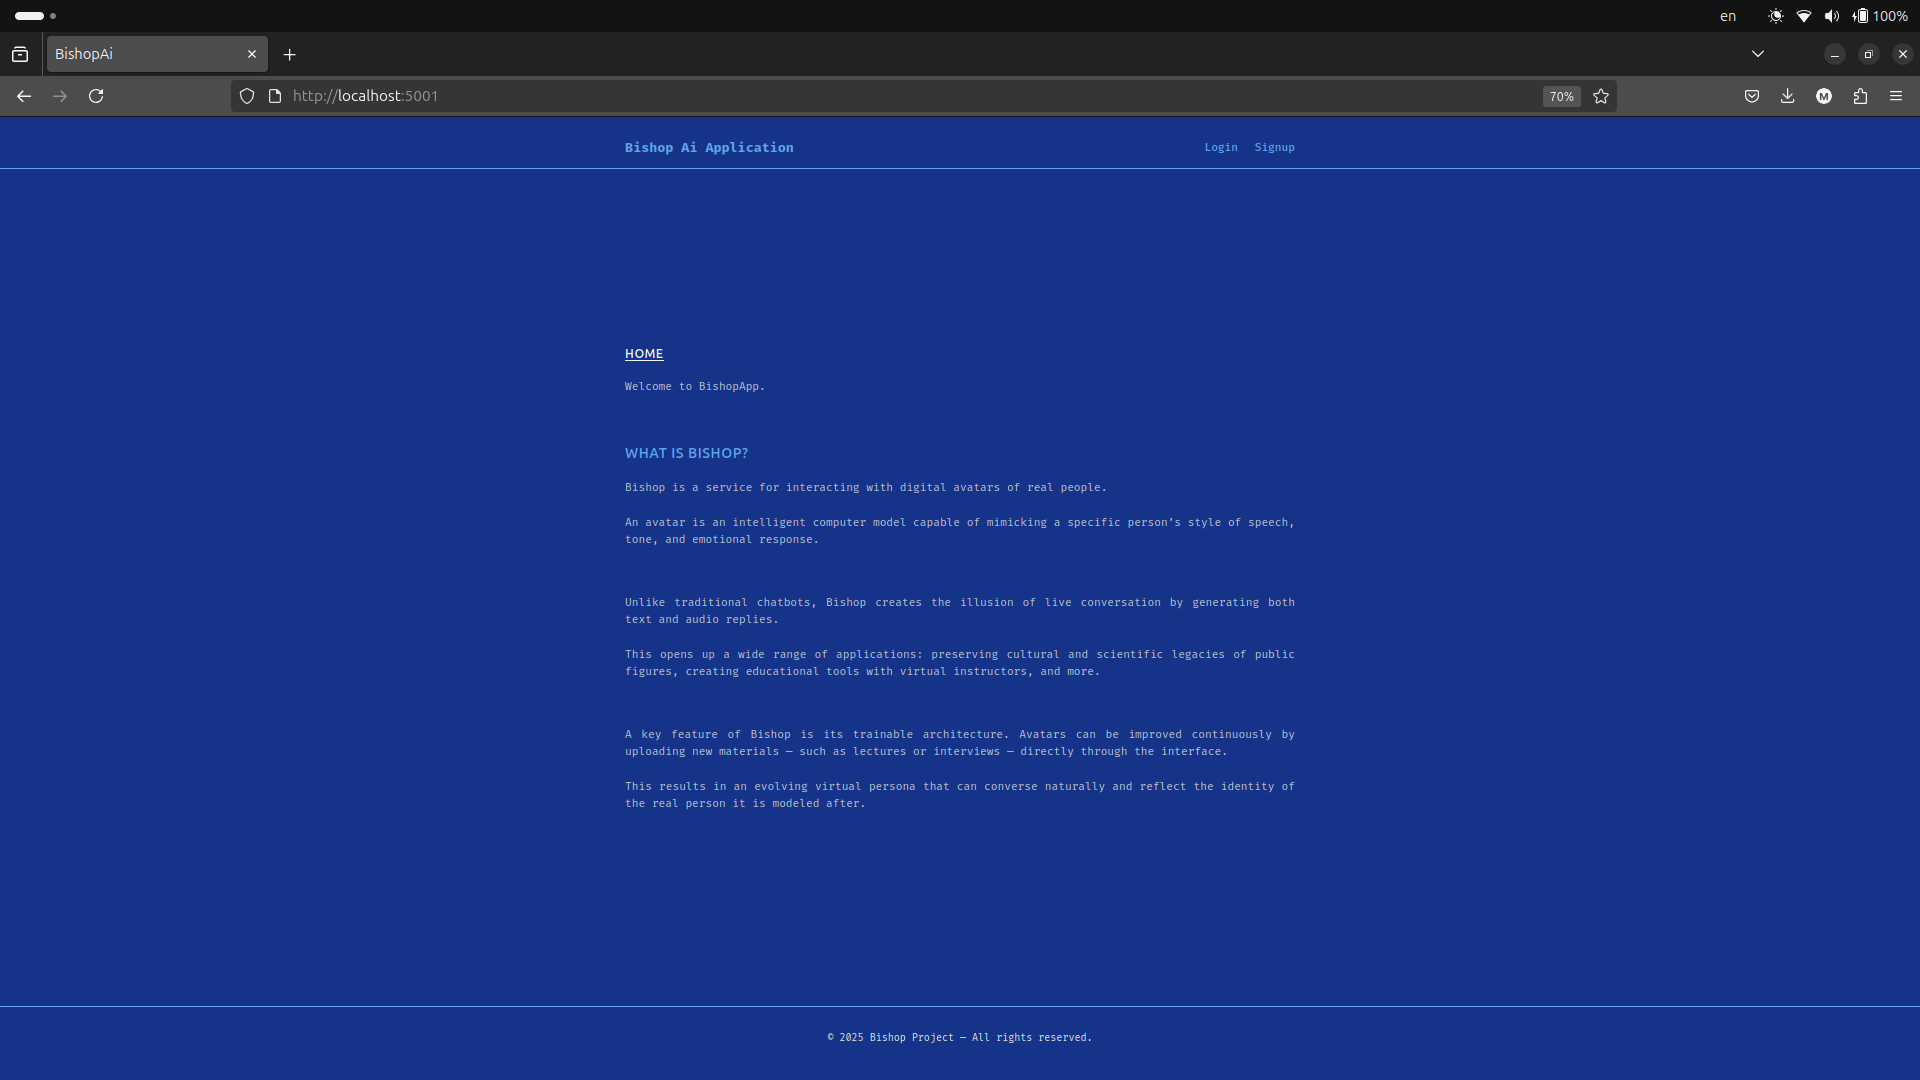
\includegraphics[width=1.0\linewidth]{images/ui/welcome.png}
    \caption{Гостевая страница}
    \label{fig:ui-page-welcome}
\end{figure}

\begin{figure}
    \centering
    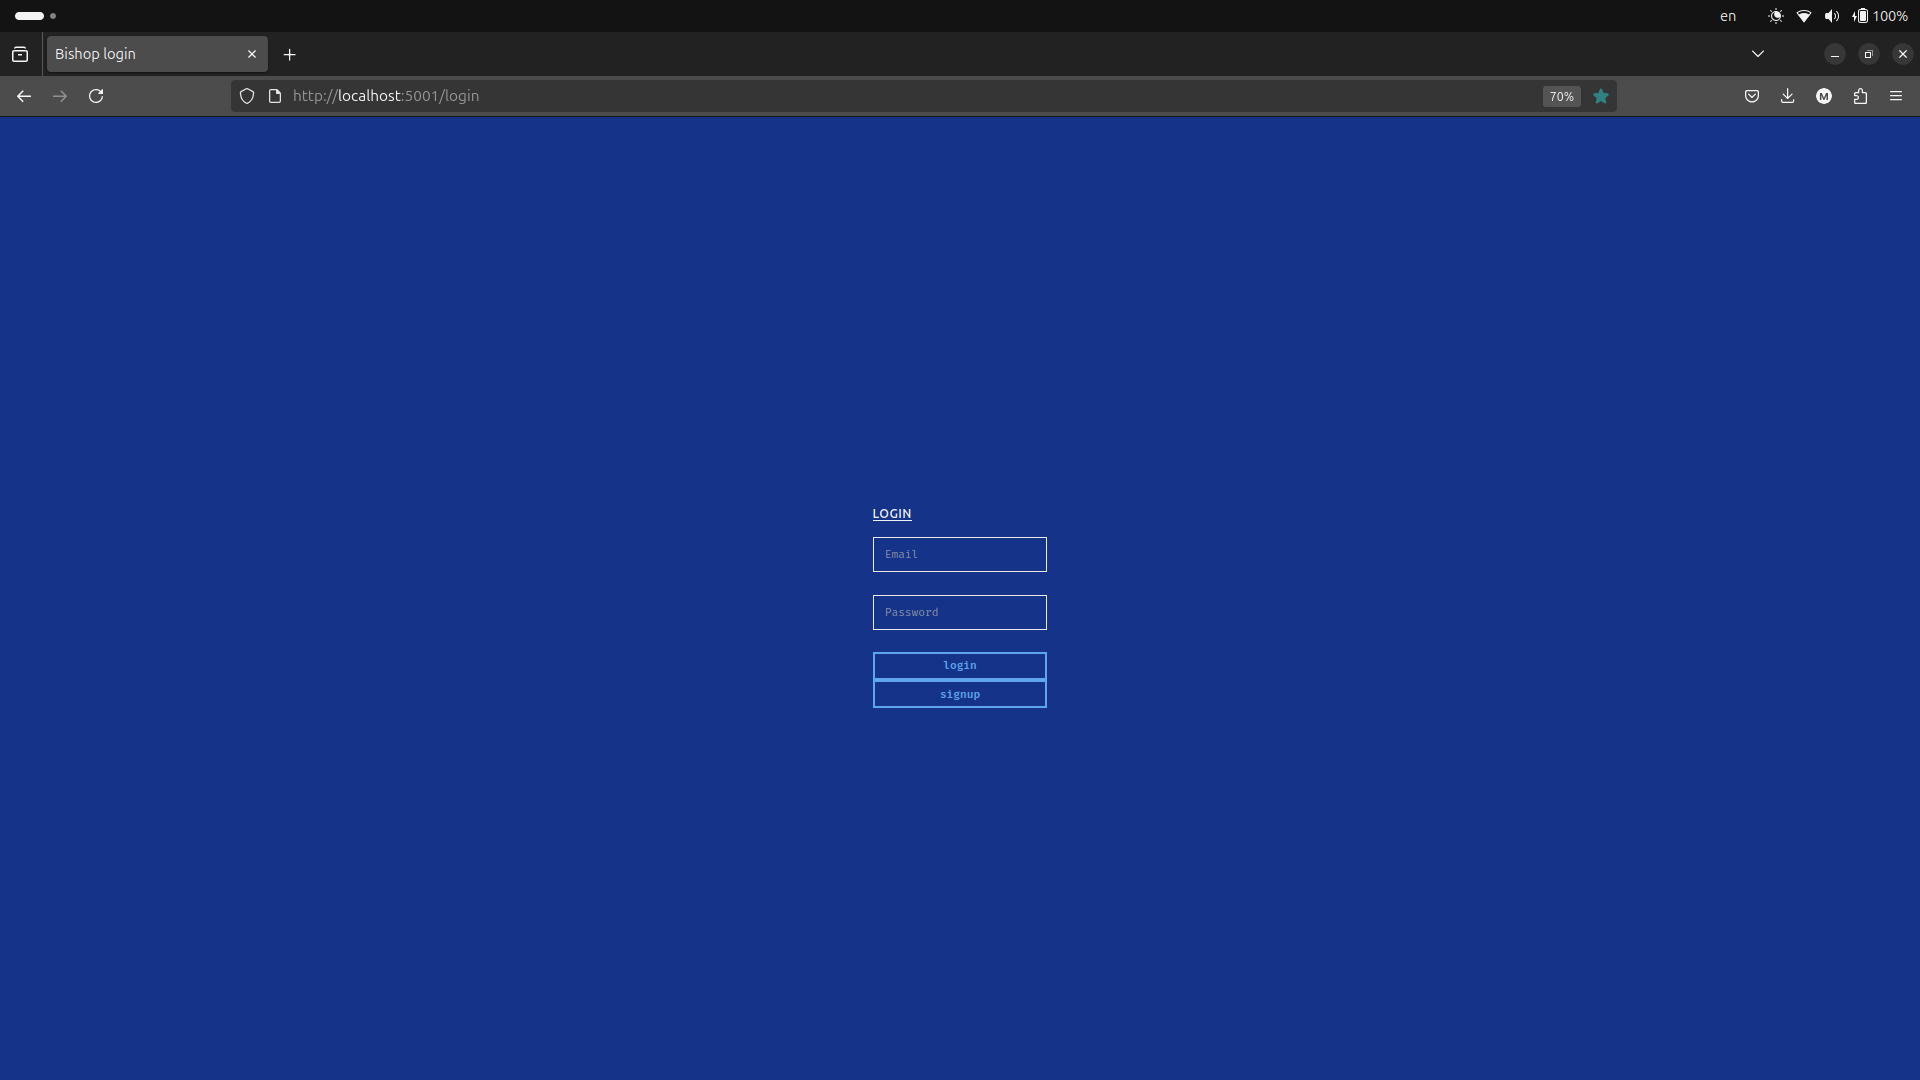
\includegraphics[width=1.0\linewidth]{images/ui/login.png}
    \caption{Страница аутентификации}
    \label{fig:ui-page-login}
\end{figure}

\begin{figure}
    \centering
    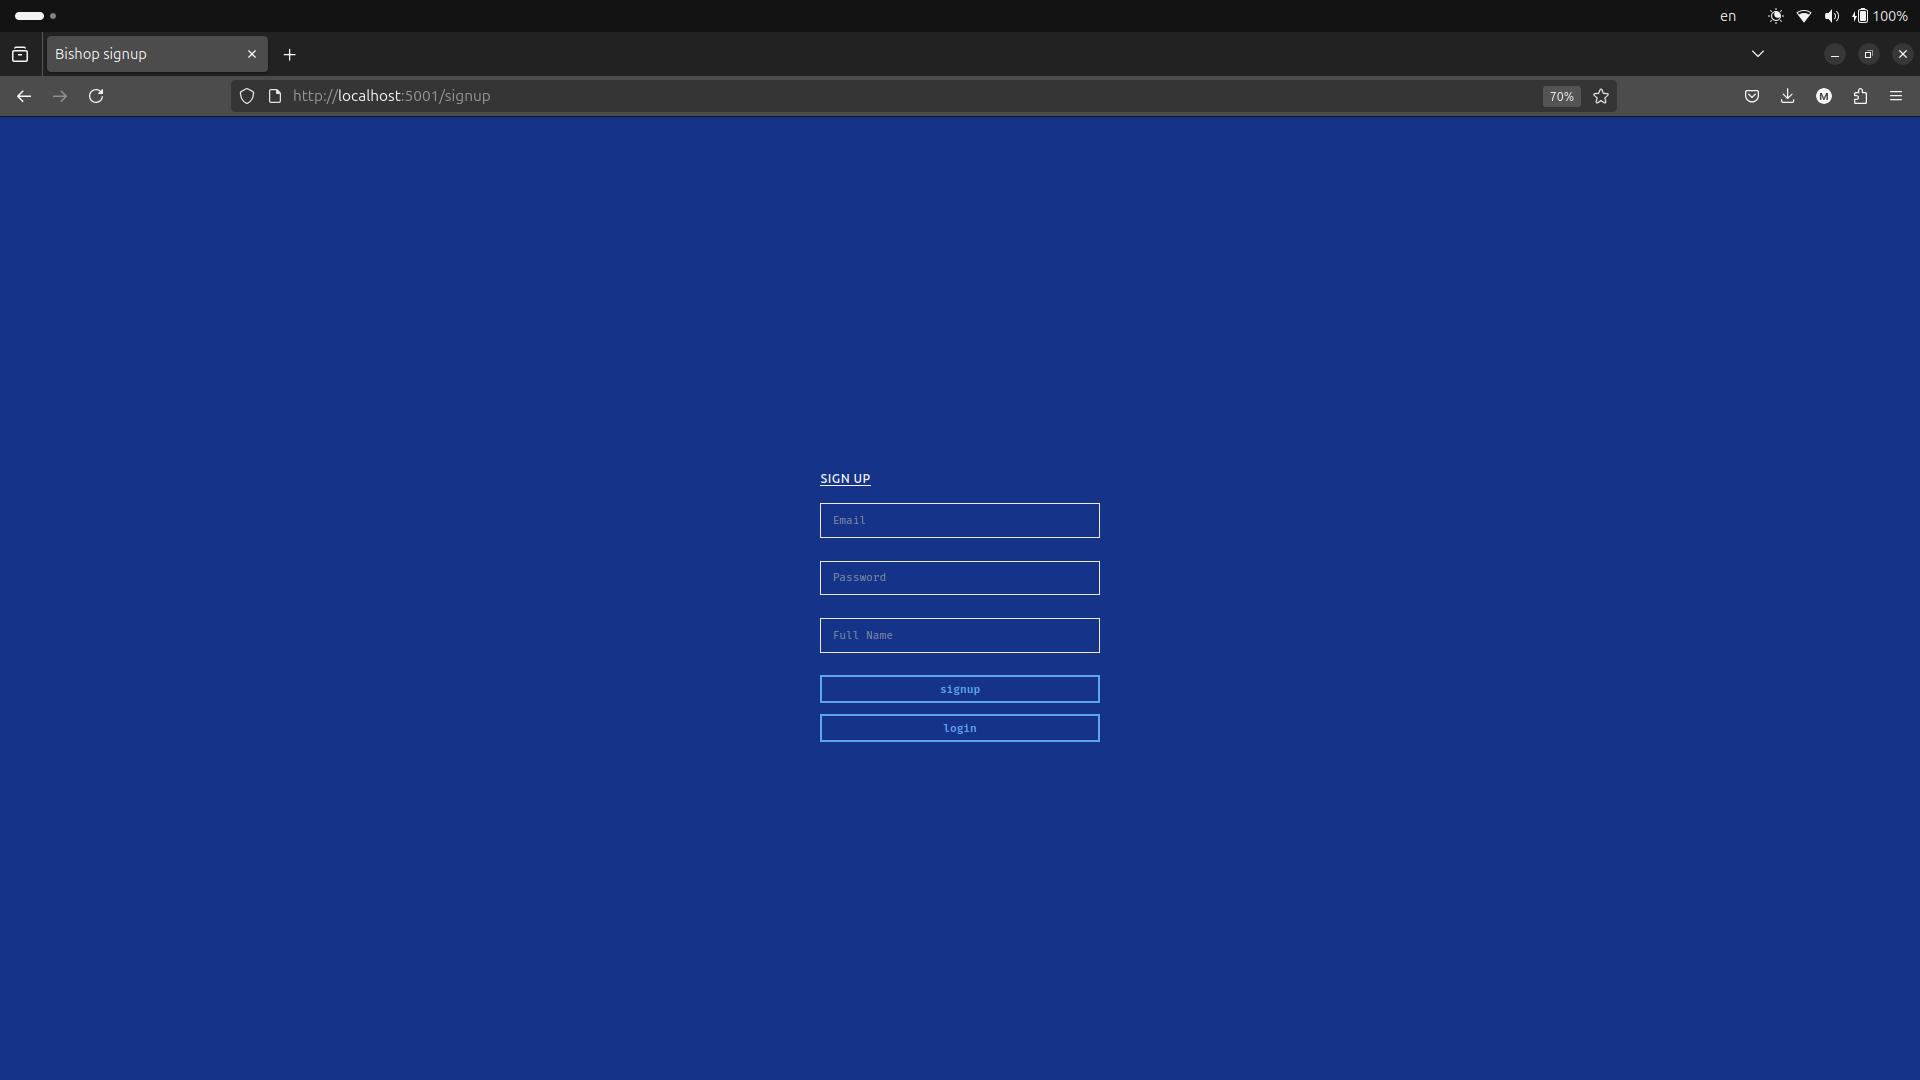
\includegraphics[width=1.0\linewidth]{images/ui/signup.png}
    \caption{Страница регистрации}
    \label{fig:ui-page-signup}
\end{figure}

\begin{figure}
    \centering
    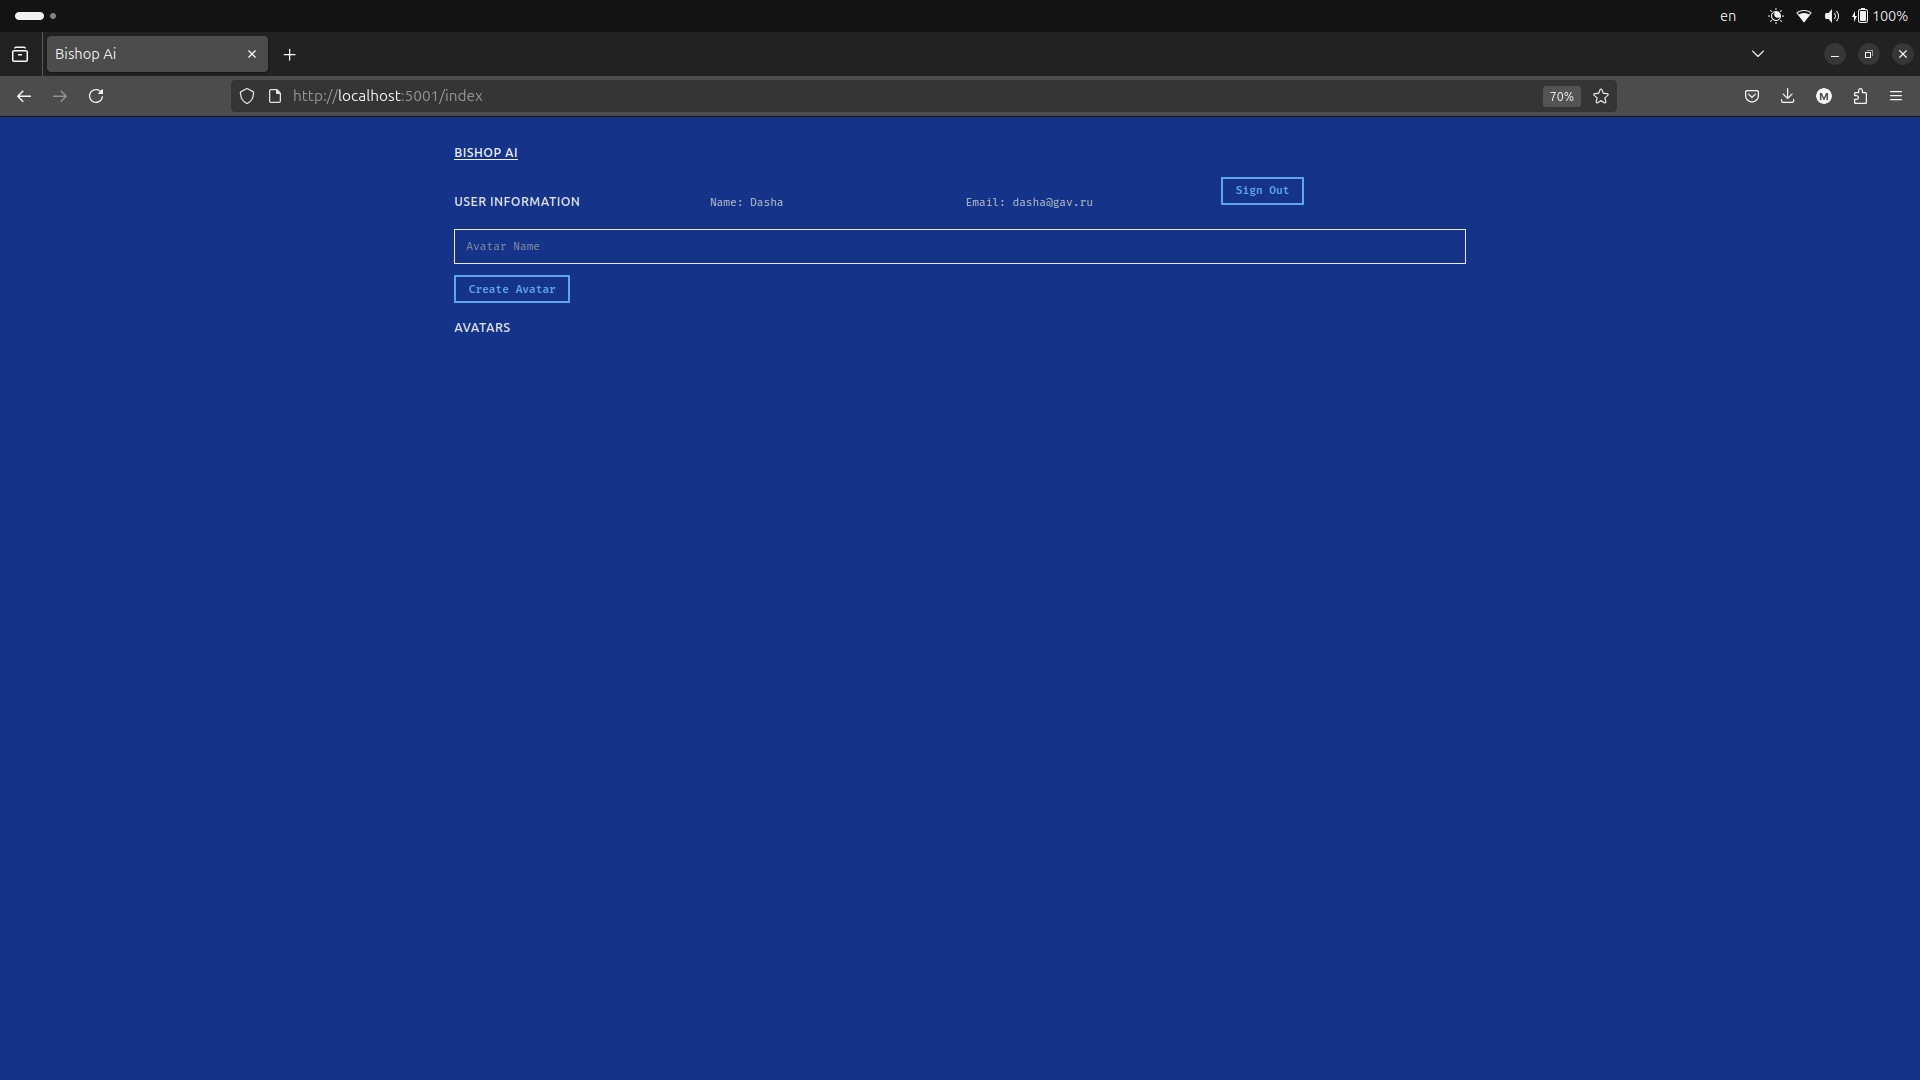
\includegraphics[width=1.0\linewidth]{images/ui/index.png}
    \caption{Основная страница приложения}
    \label{fig:ui-page-index}
\end{figure}

\begin{figure}
    \centering
    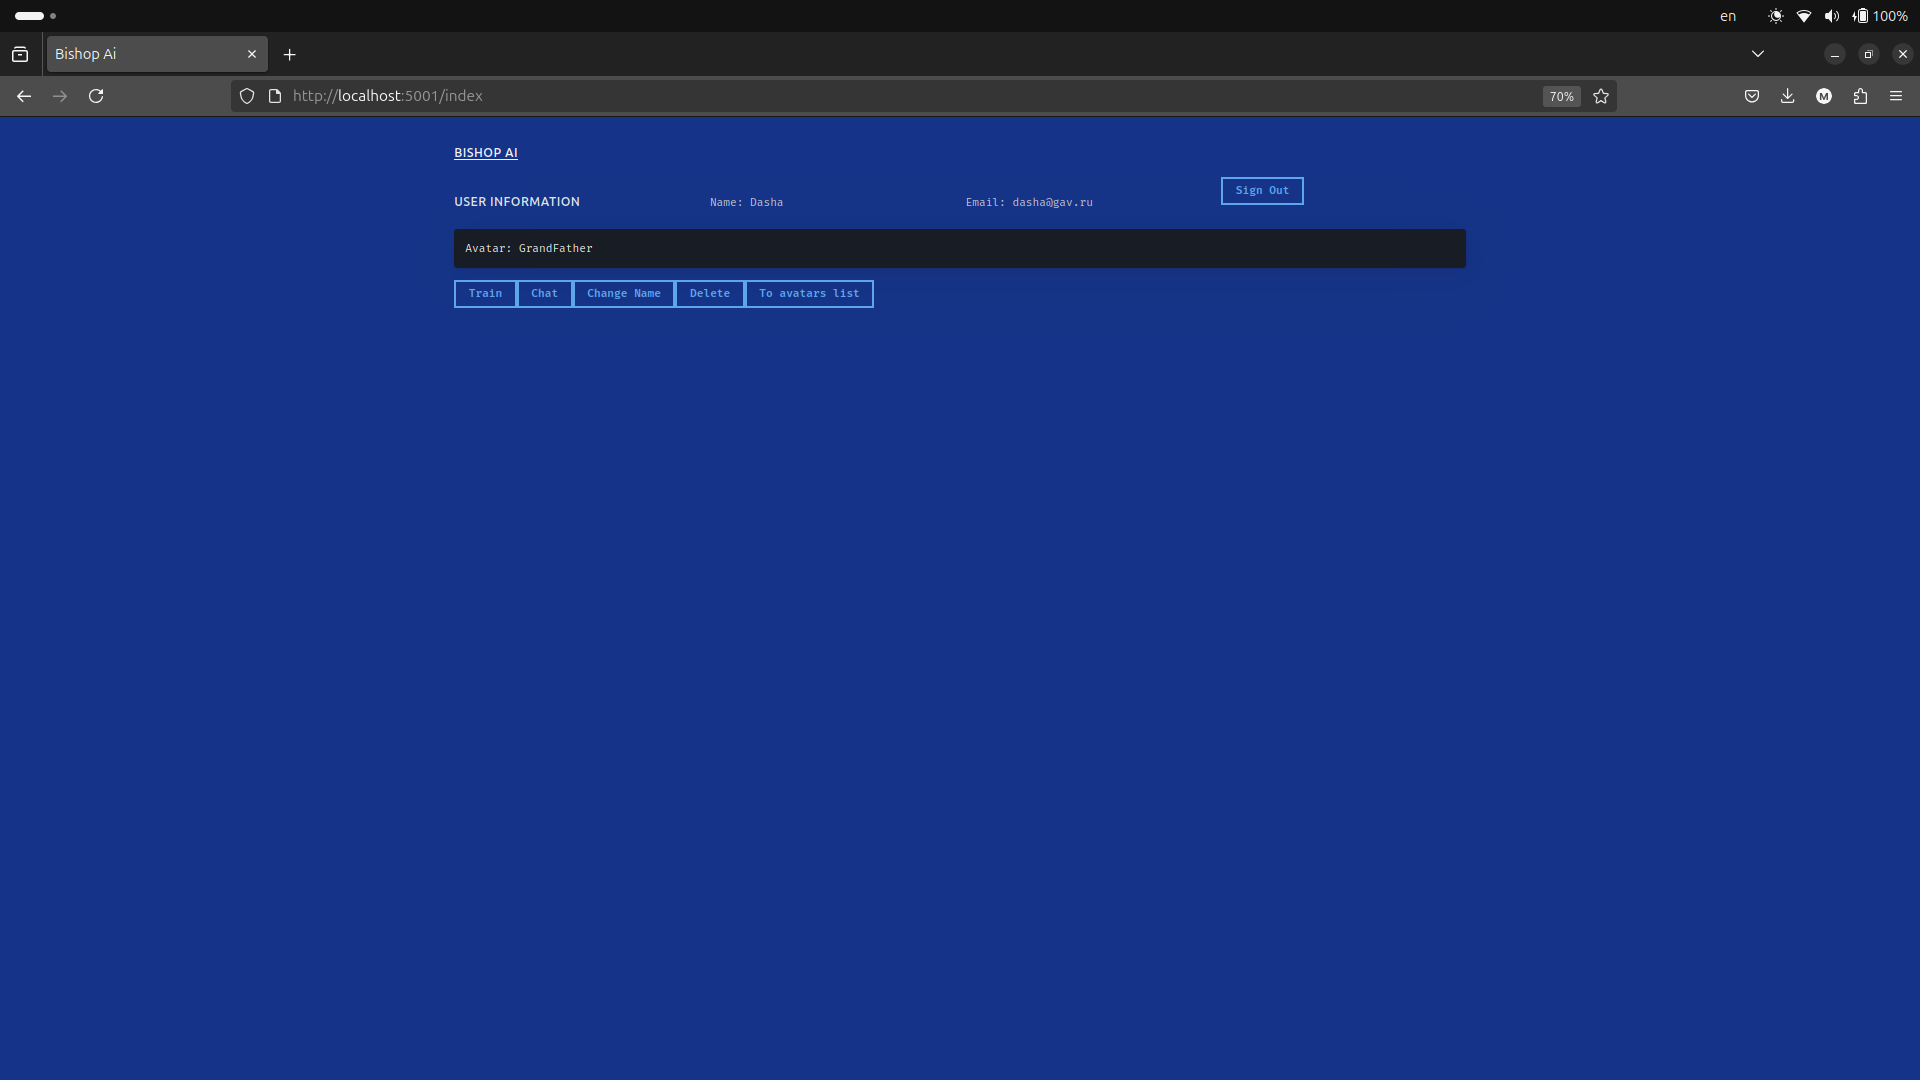
\includegraphics[width=1.0\linewidth]{images/ui/avatar.png}
    \caption{Страница управления аватарами}
    \label{fig:ui-page-avatar}
\end{figure}

\begin{figure}
    \centering
    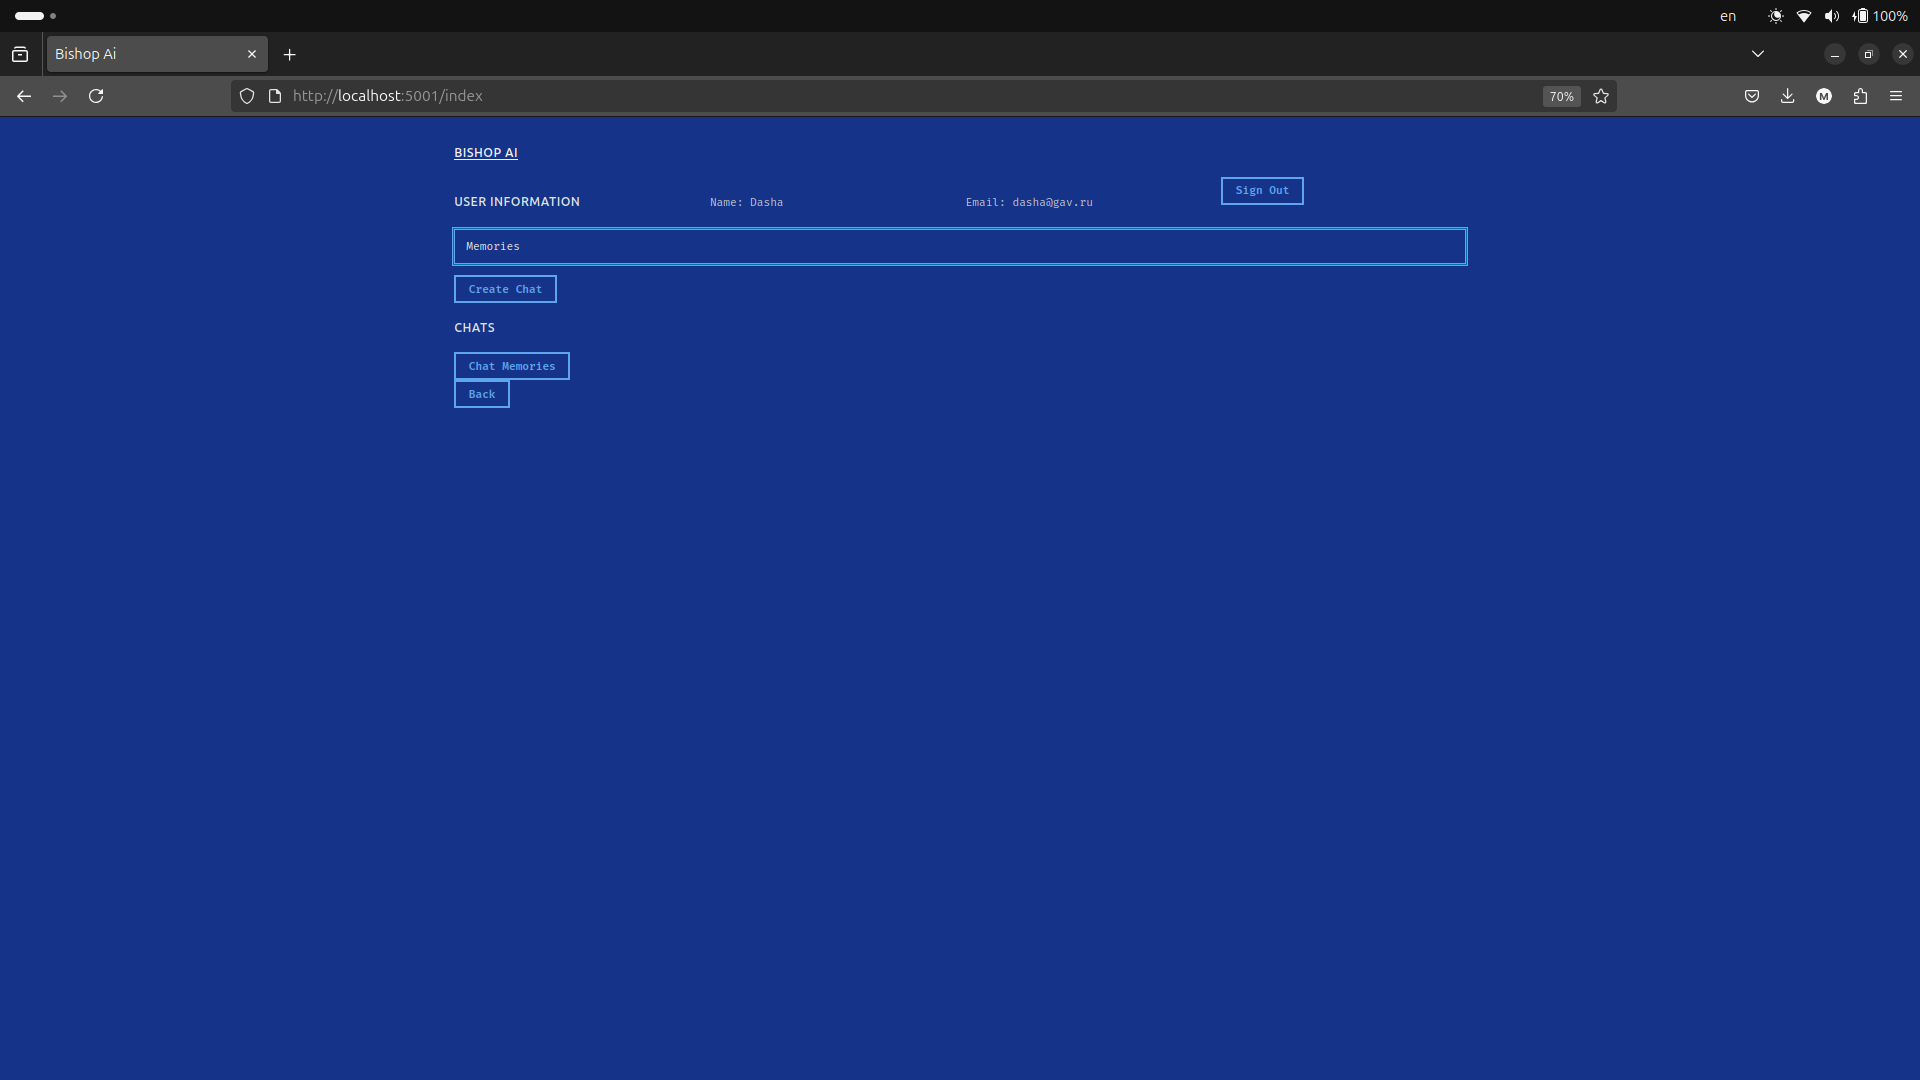
\includegraphics[width=1.0\linewidth]{images/ui/chat1.png}
    \caption{Страница управления чатами}
    \label{fig:ui-page-chat1}
\end{figure}

\begin{figure}
    \centering
    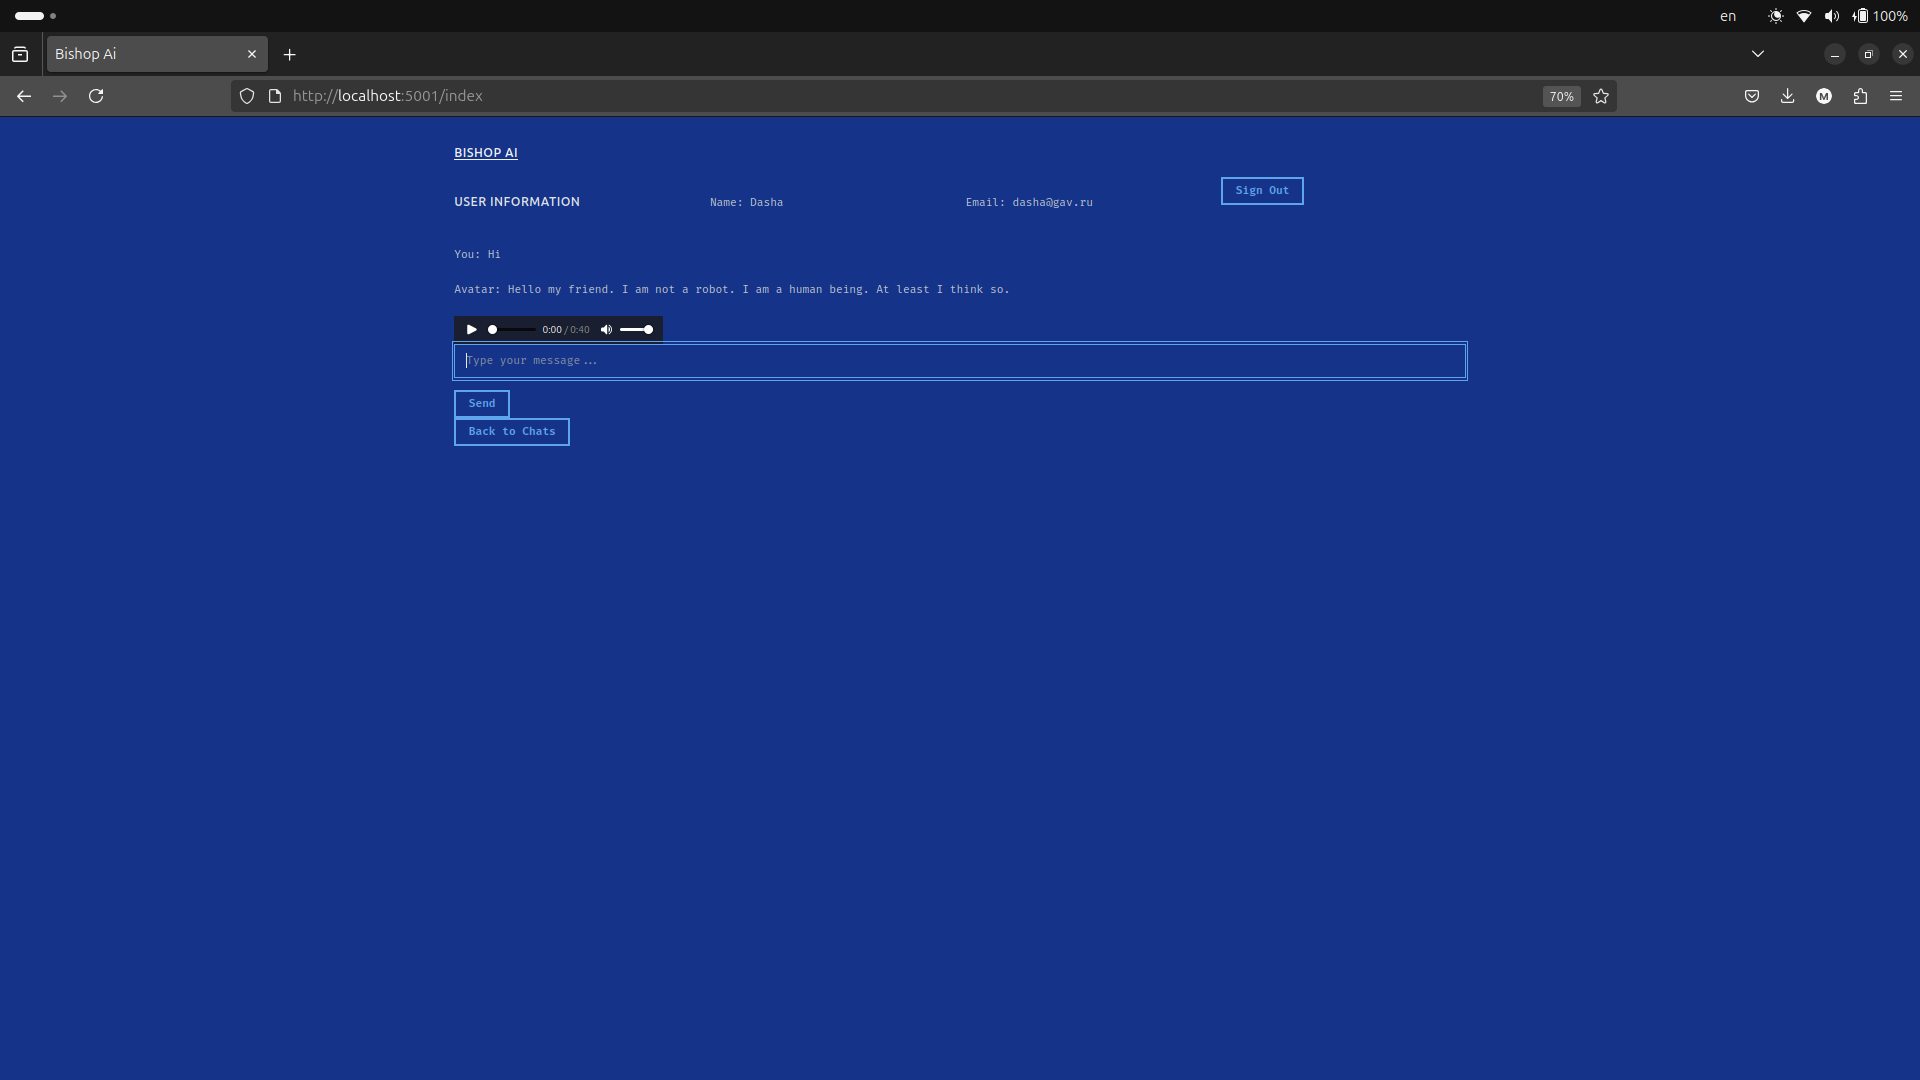
\includegraphics[width=1.0\linewidth]{images/ui/chat2.png}
    \caption{Страница чата}
    \label{fig:ui-page-chat2}
\end{figure}

\begin{figure}
    \centering
    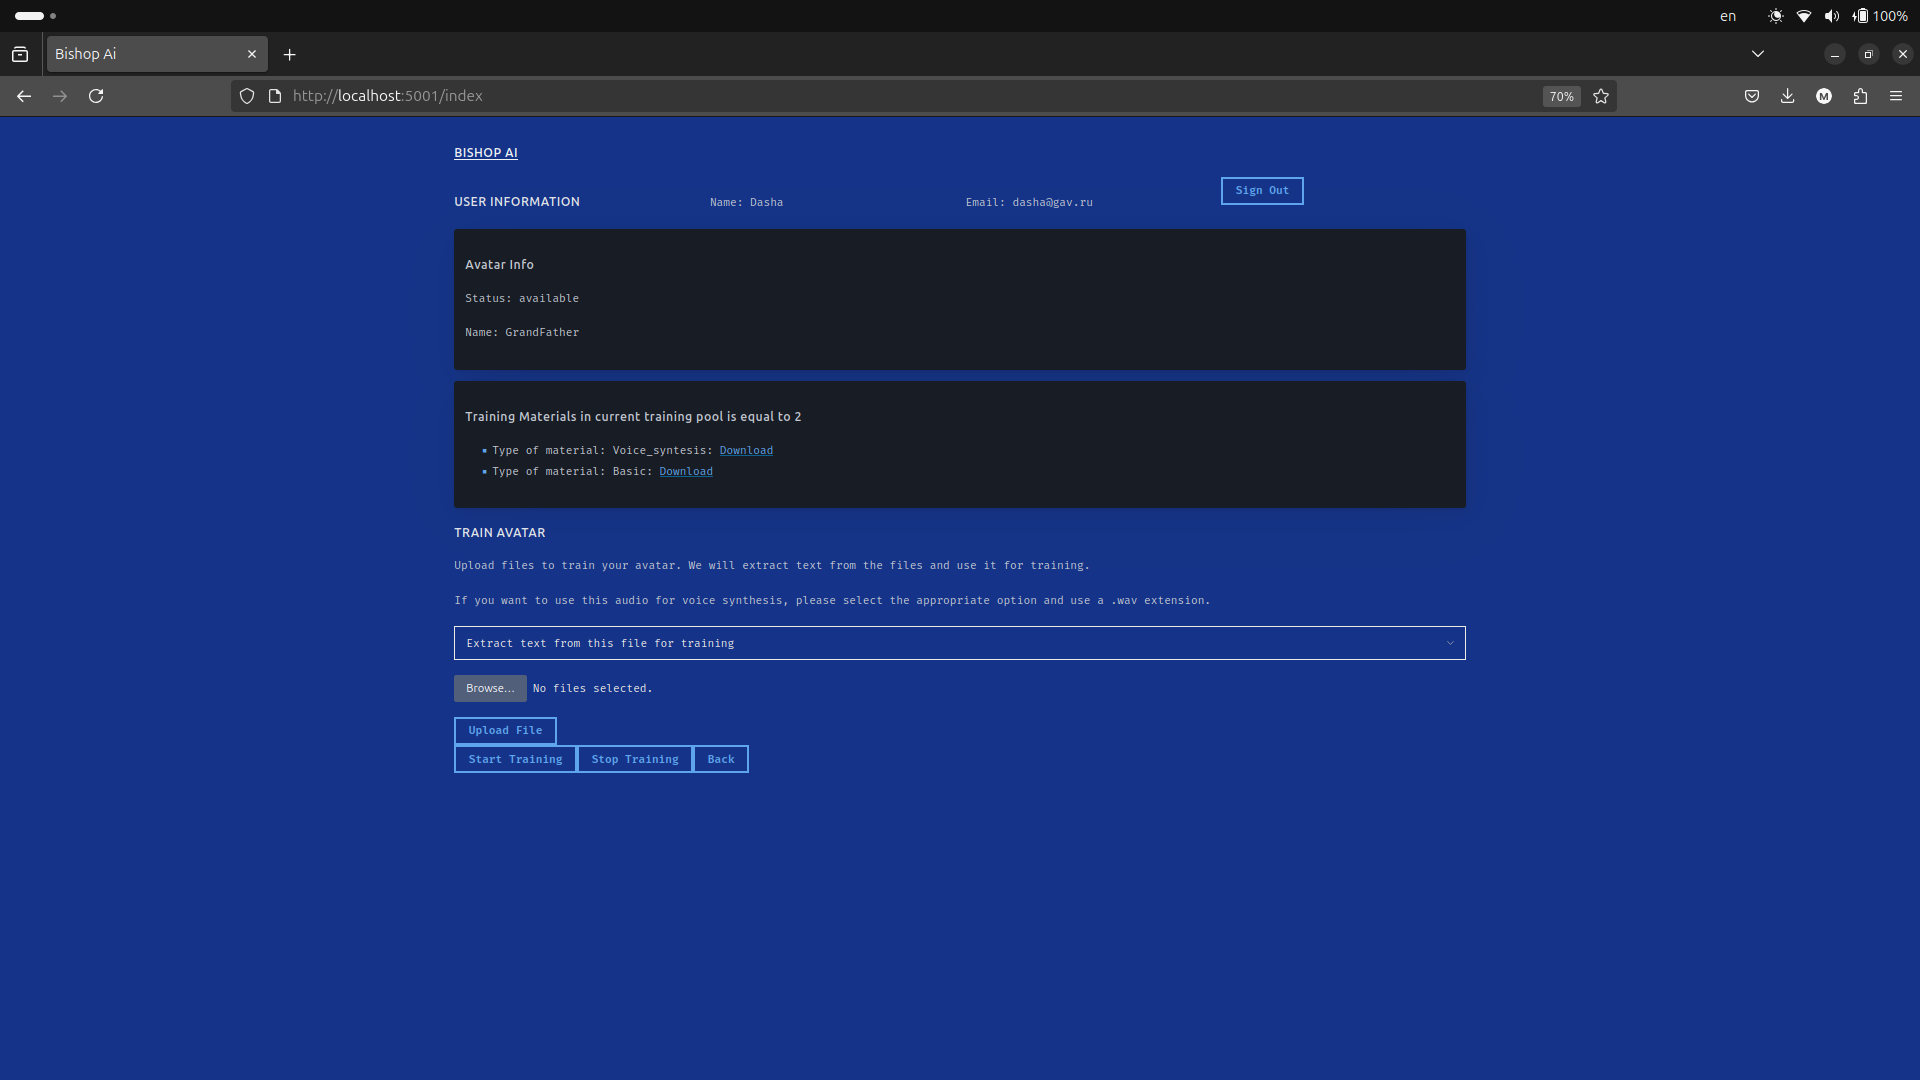
\includegraphics[width=1.0\linewidth]{images/ui/train.png}
    \caption{Интерфейс обучения аватара}
    \label{fig:ui-page-train}
\end{figure}

\chapter{Отчёты о работе сервиса}\label{app:B}

\begin{figure}[h!]
    \centering
    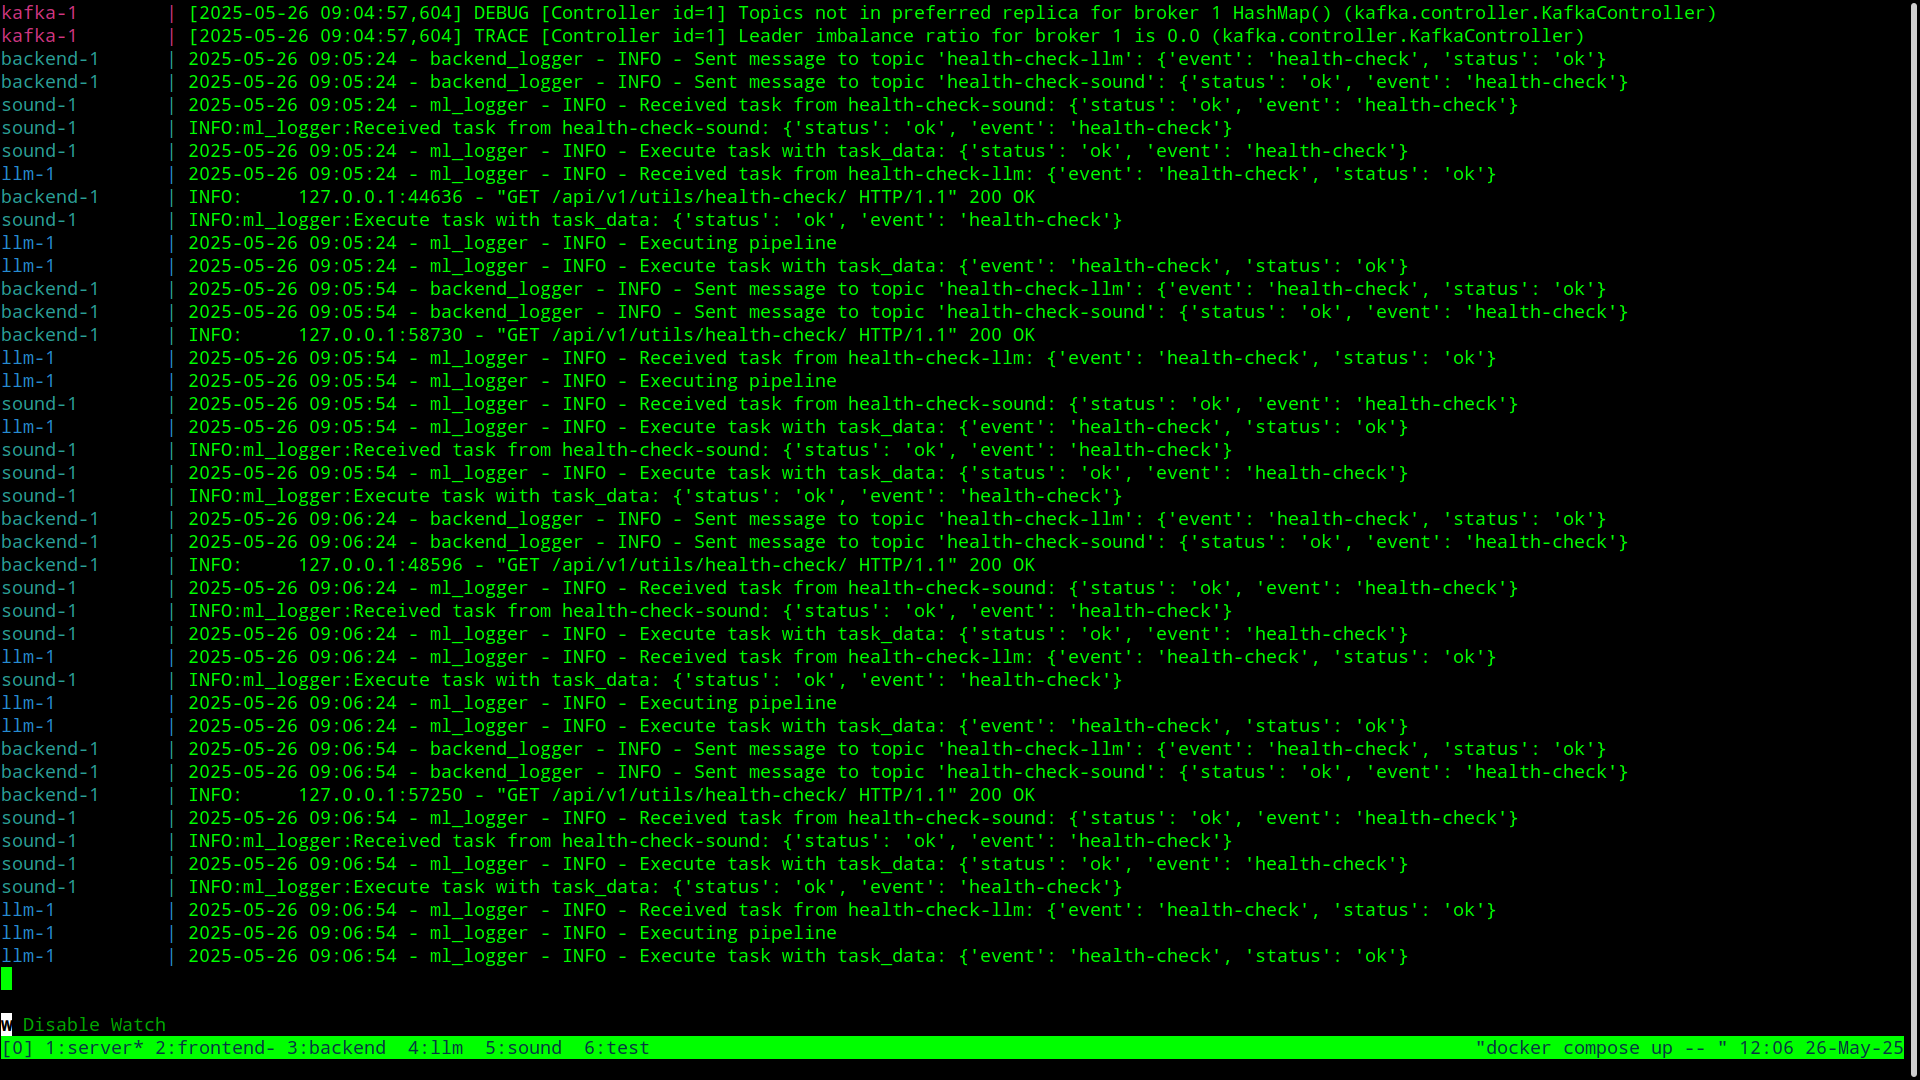
\includegraphics[width=1.0\linewidth]{images/results/health-check.png}
    \caption{Фрагмент логов инициализации системы и периодической проверки состояния доступности системы}
    \label{fig:res-healt-check}
\end{figure}

\begin{figure}
    \centering
    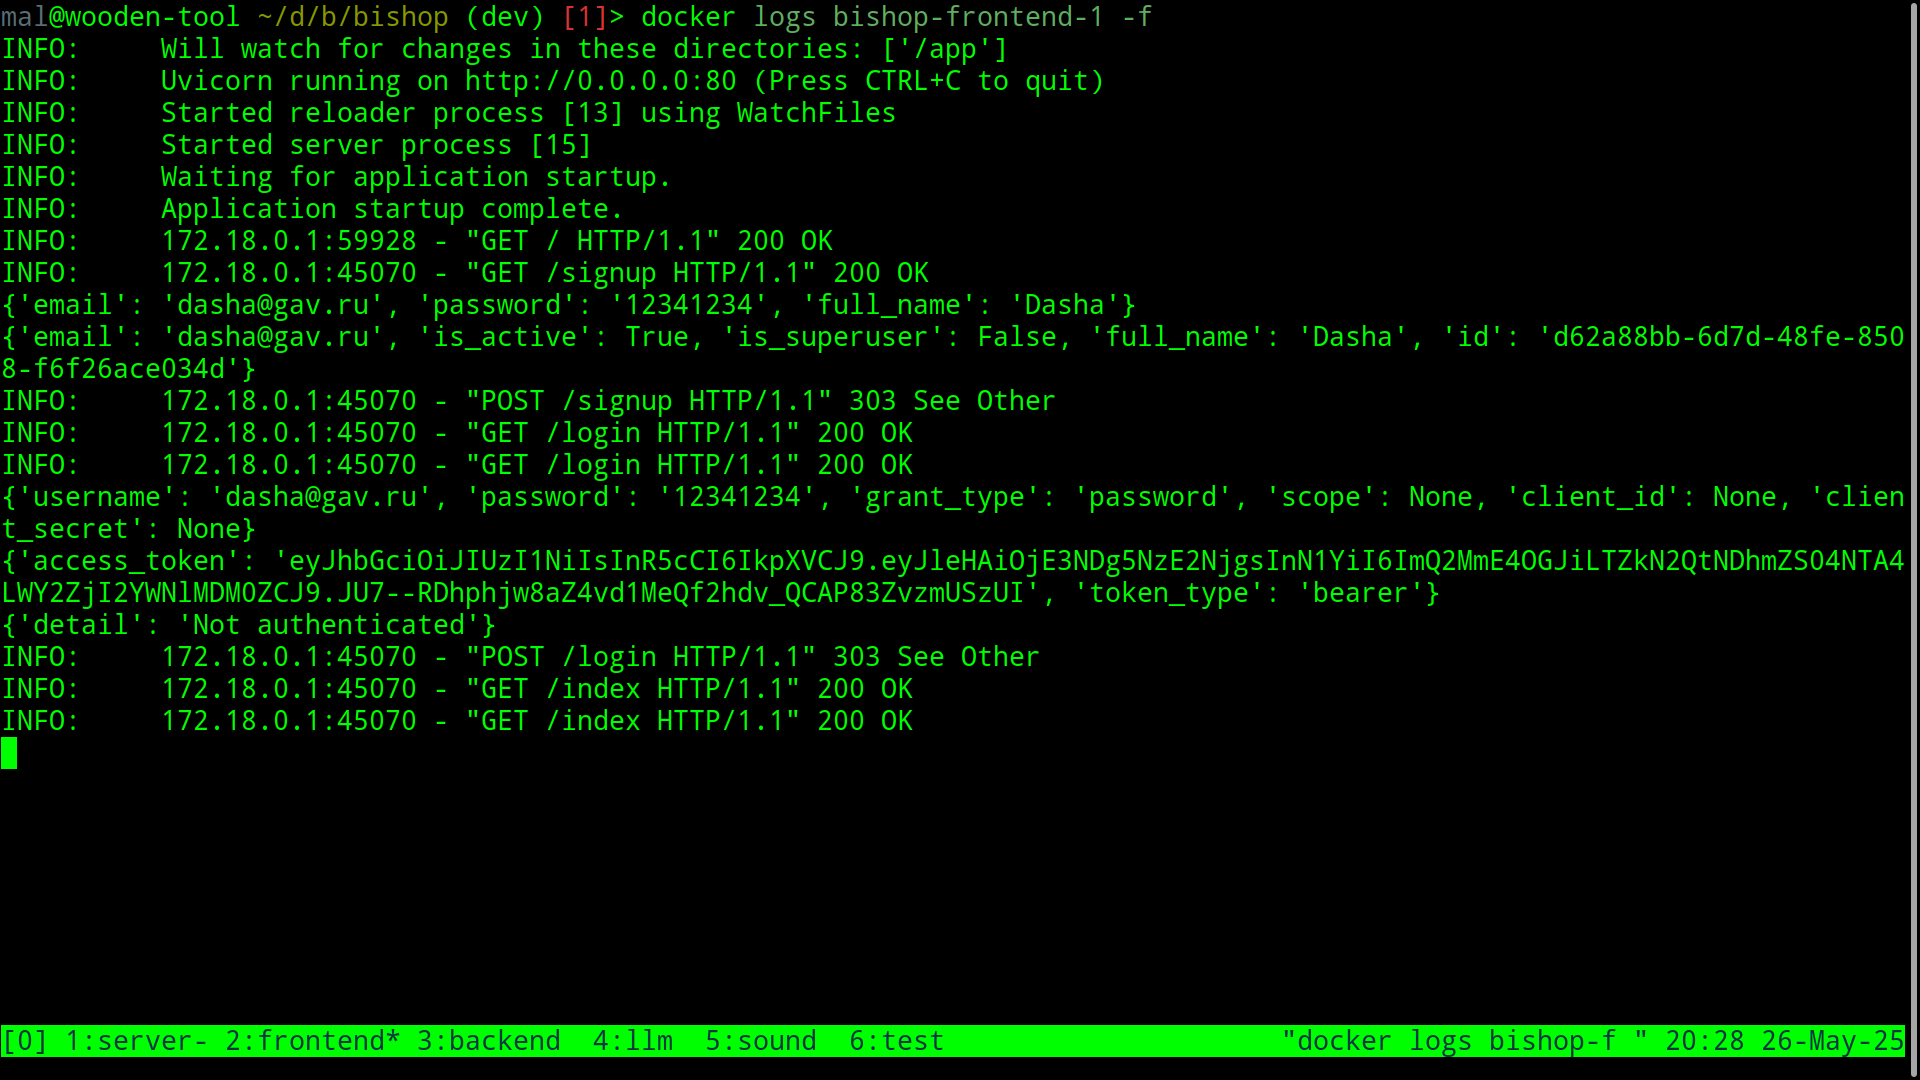
\includegraphics[width=1.0\linewidth]{images/results/signup-login-frontend.png}
    \caption{Регистрация и авторизация пользователя}
    \label{fig:res-signup-login-frontend}
\end{figure}

\begin{figure}
    \centering
    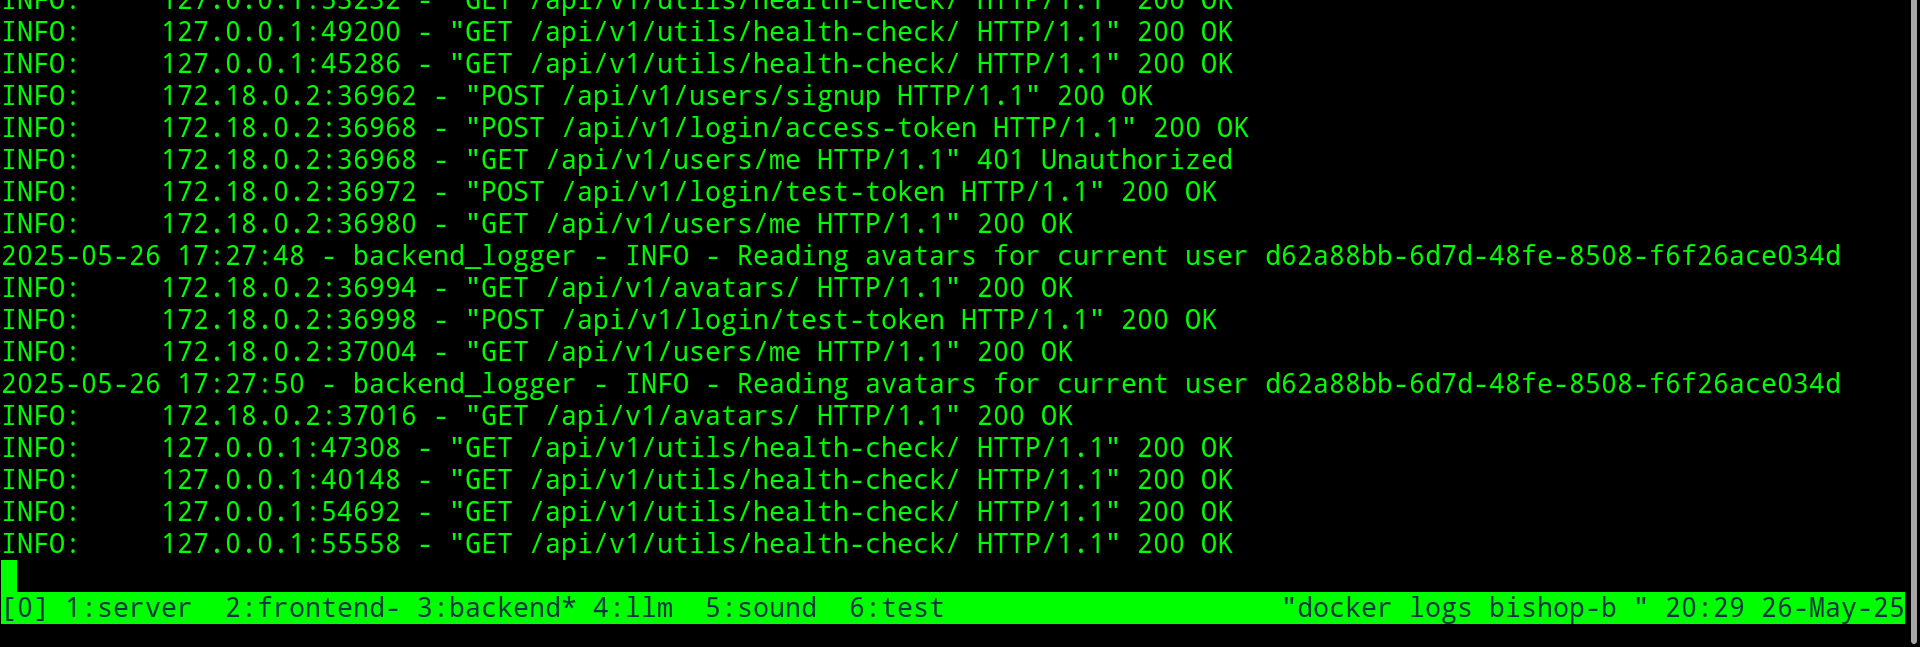
\includegraphics[width=1.0\linewidth]{images/results/signup-login-backend.png}
    \caption{Обработка регистрации и авторизации на стороне backend-сервиса}
    \label{fig:res-signup-login-backend}
\end{figure}

\begin{figure}
    \centering
    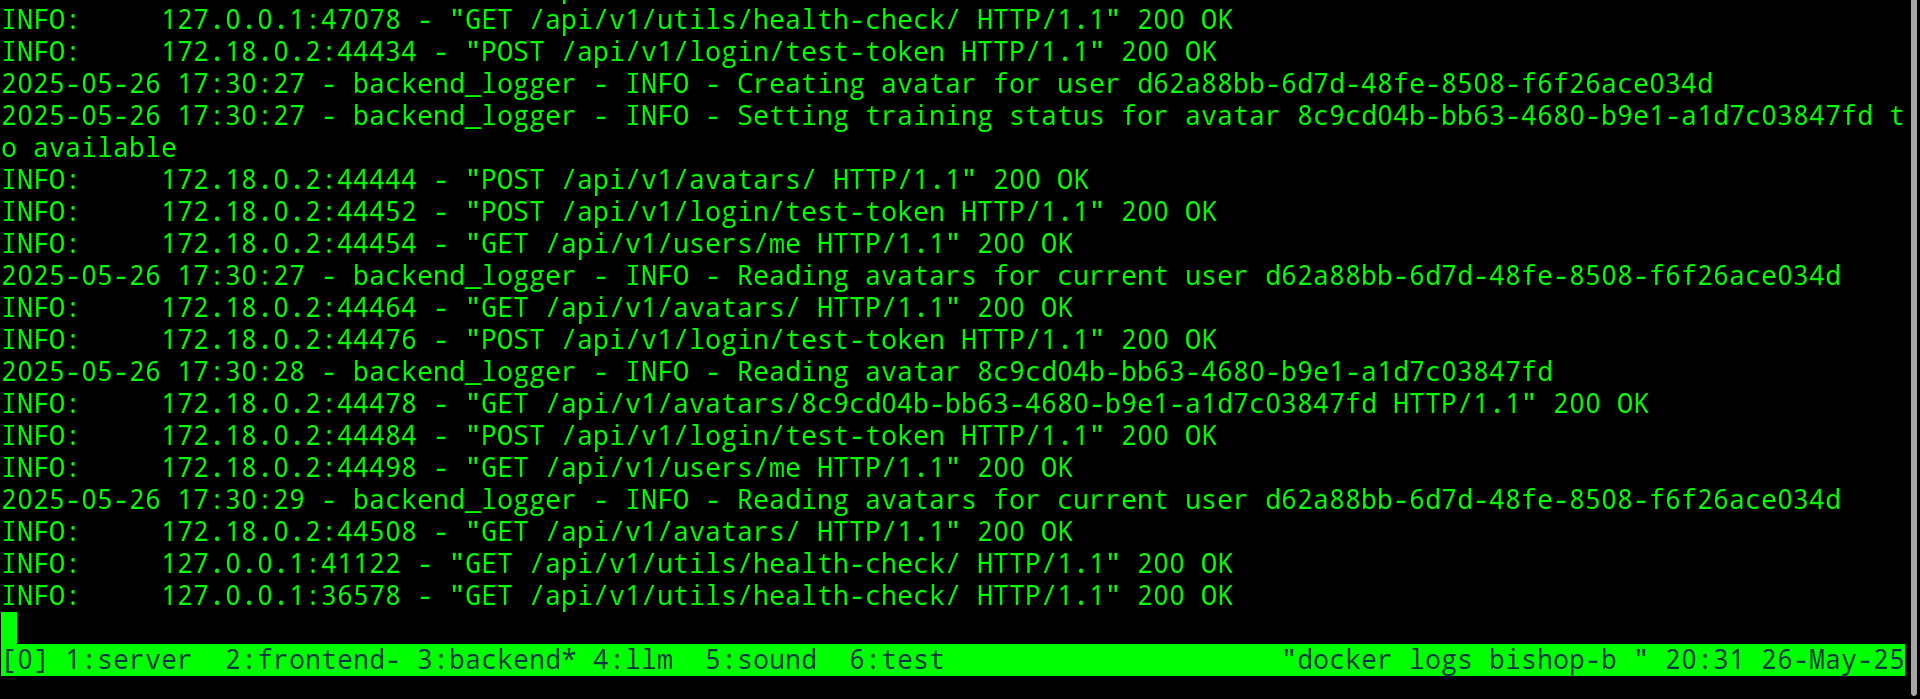
\includegraphics[width=1.0\linewidth]{images/results/bk-create-avatar.png}
    \caption{Создание нового цифрового аватара пользователем}
    \label{fig:res-bk-create-avatar}
\end{figure}

\begin{figure}
    \centering
    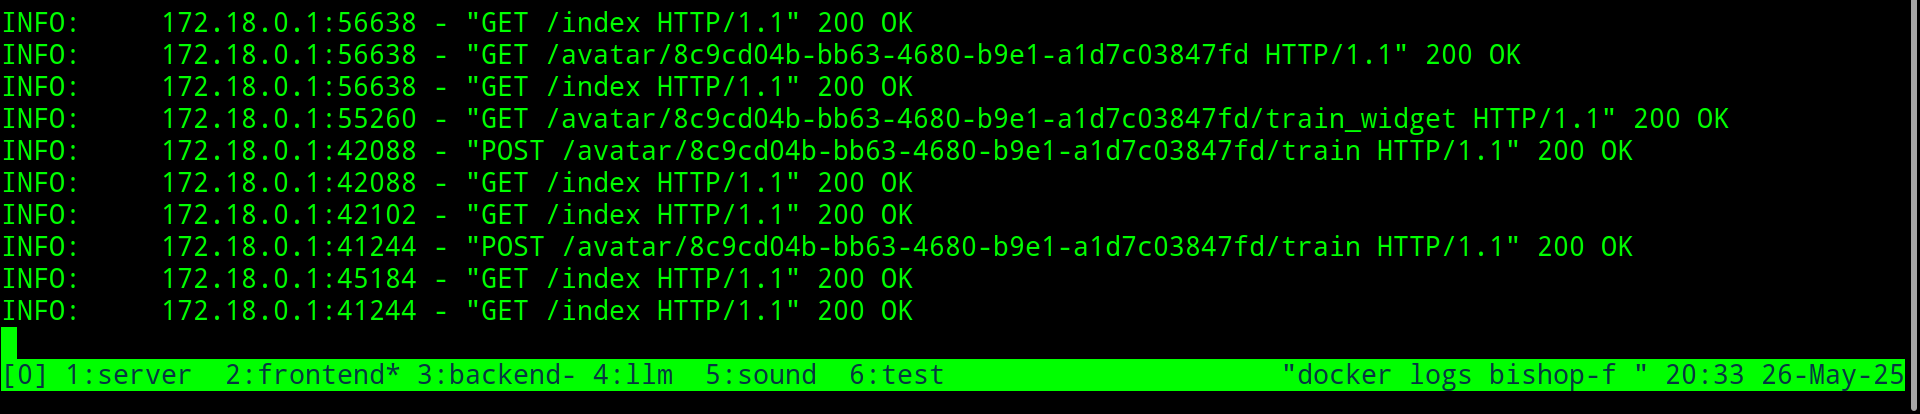
\includegraphics[width=1.0\linewidth]{images/results/fr-upload-materials.png}
    \caption{Загрузка текстовых и аудиофайлов через интерфейс}
    \label{fig:res-fr-upload-materials}
\end{figure}

\begin{figure}
    \centering
    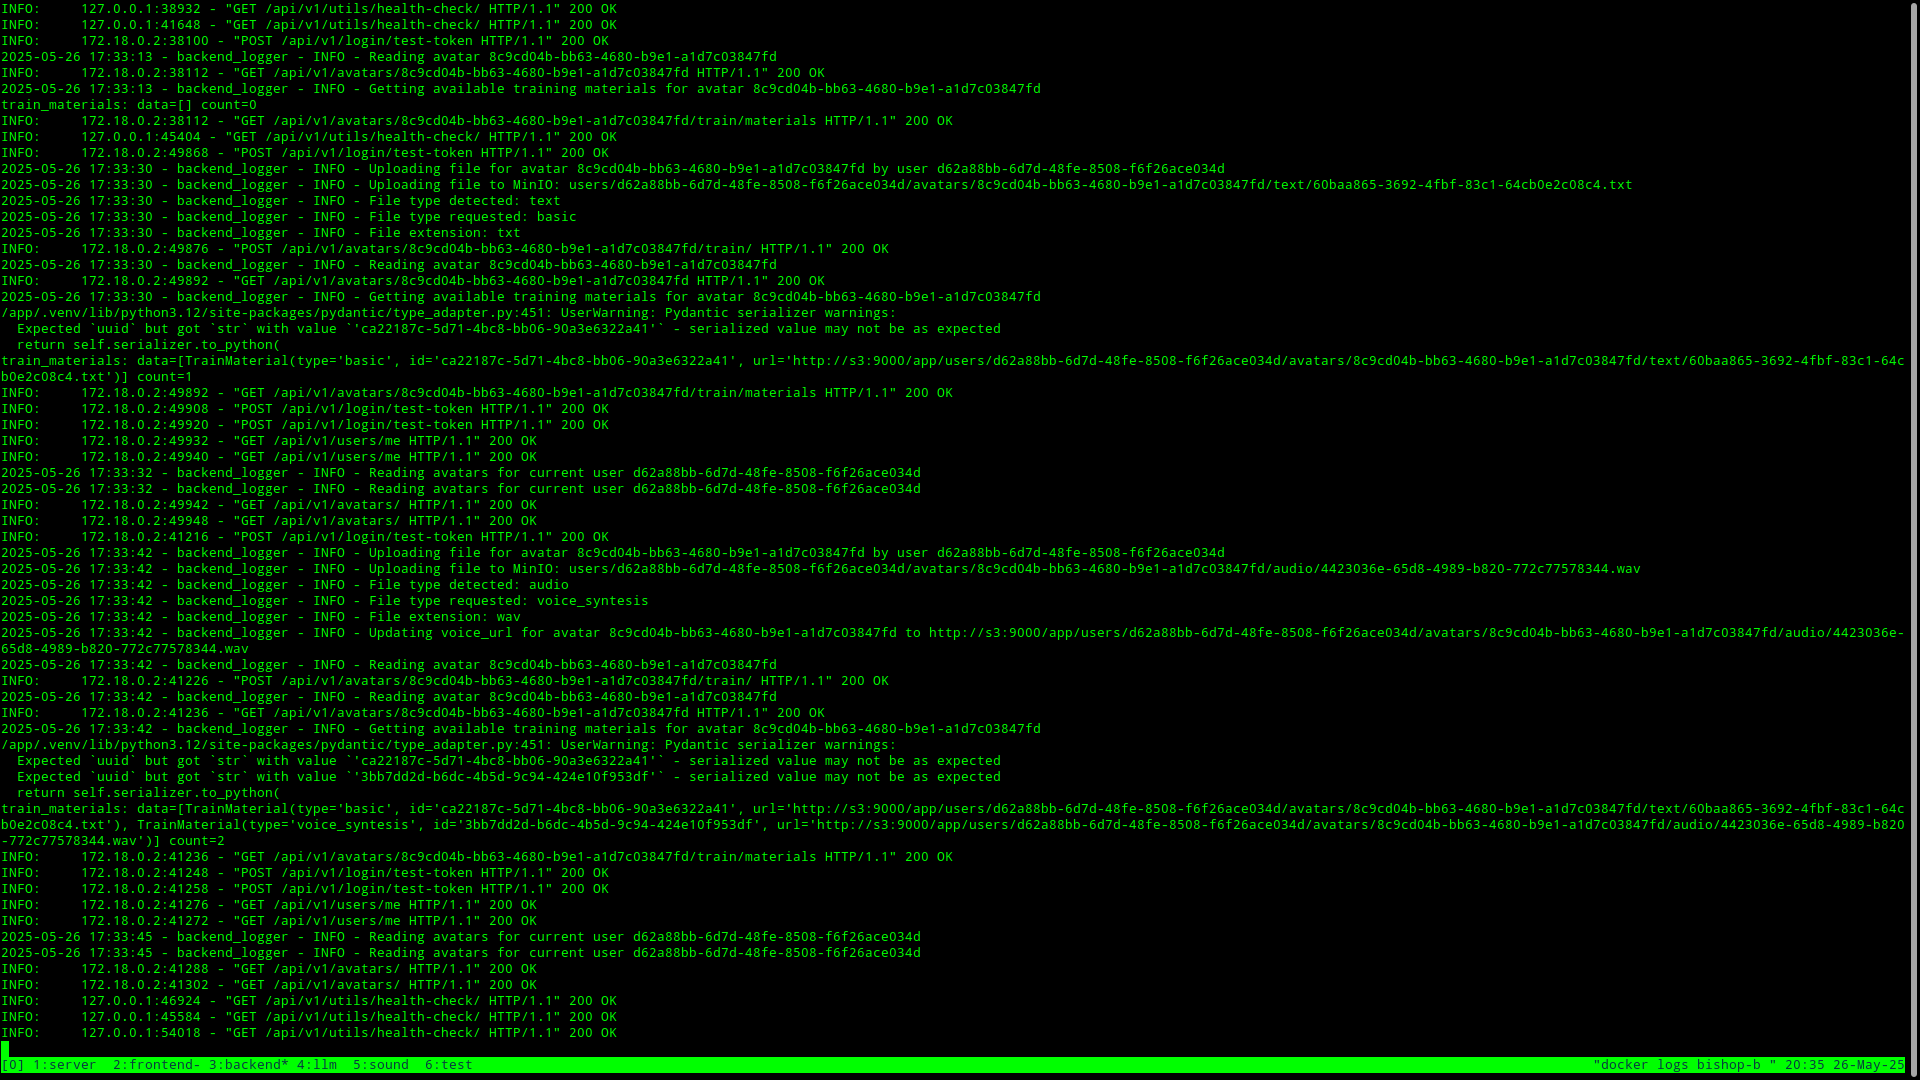
\includegraphics[width=1.0\linewidth]{images/results/bk-upload-materials.png}
    \caption{Фиксация и сохранение обучающих материалов на стороне backend}
    \label{fig:res-bk-upload-materials}
\end{figure}

\begin{figure}
    \centering
    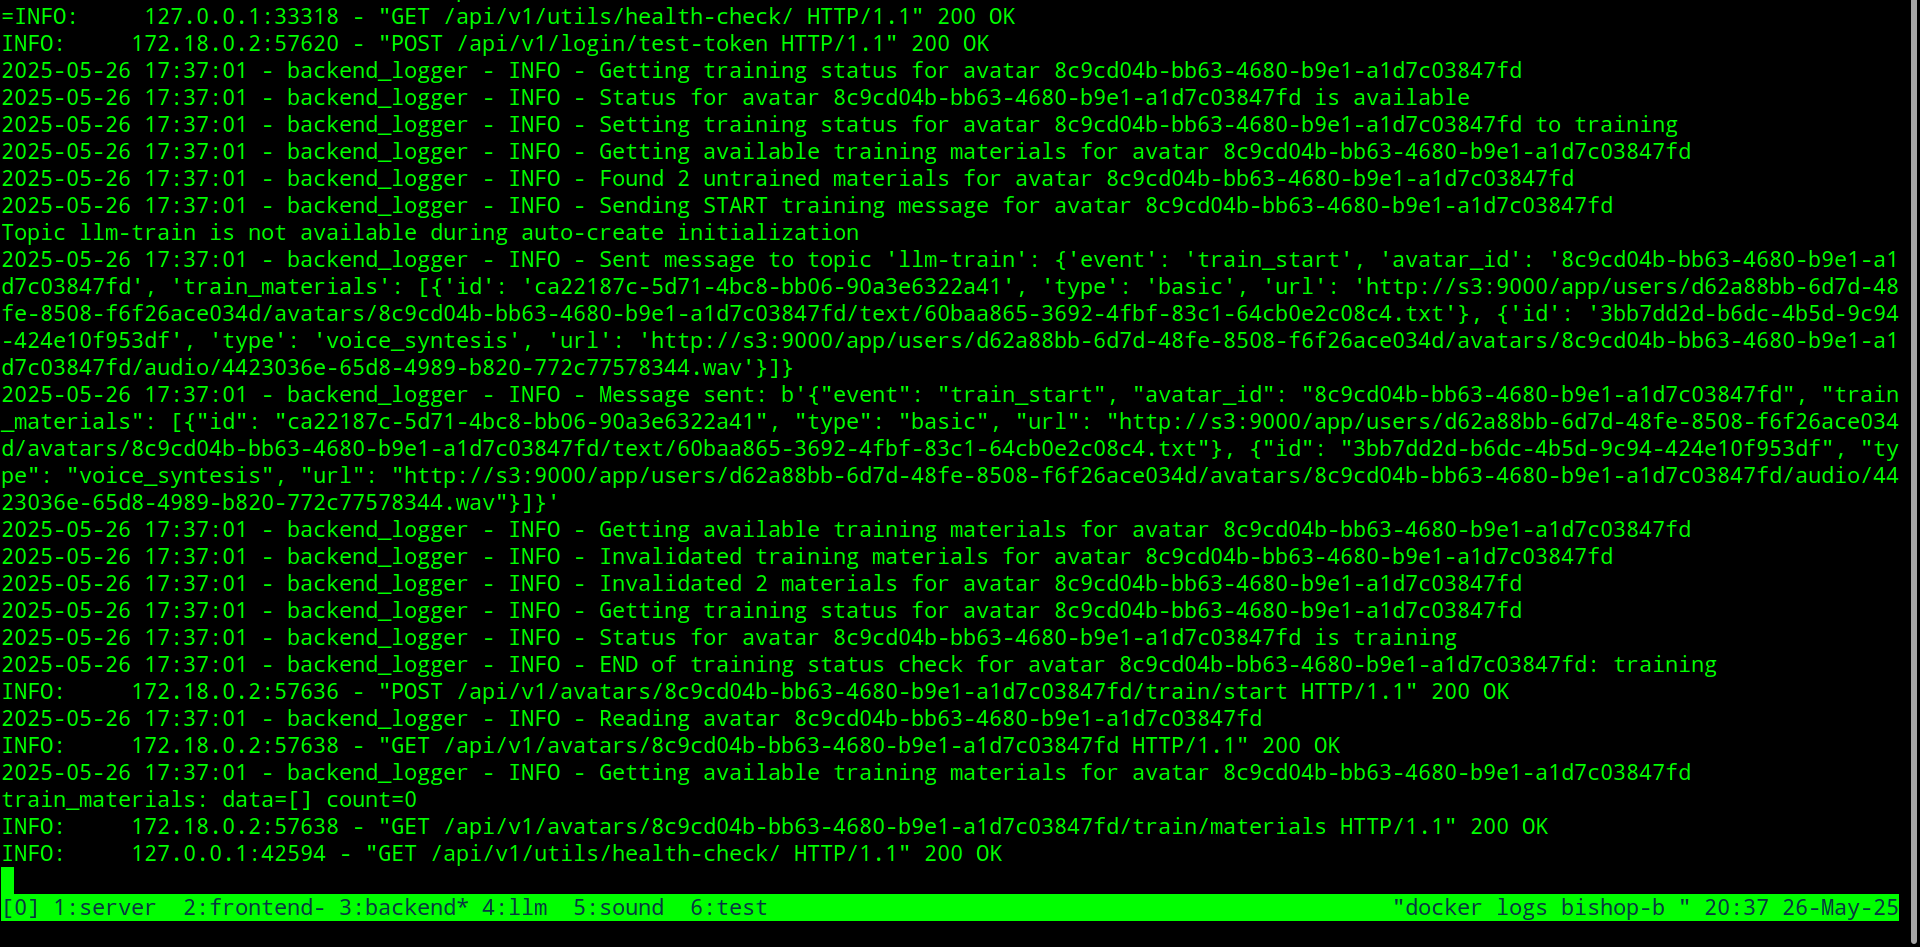
\includegraphics[width=1.0\linewidth]{images/results/bk-start-train.png}
    \caption{Инициация процесса обучения через backend}
    \label{fig:res-bk-start-train}
\end{figure}

\begin{figure}
    \centering
    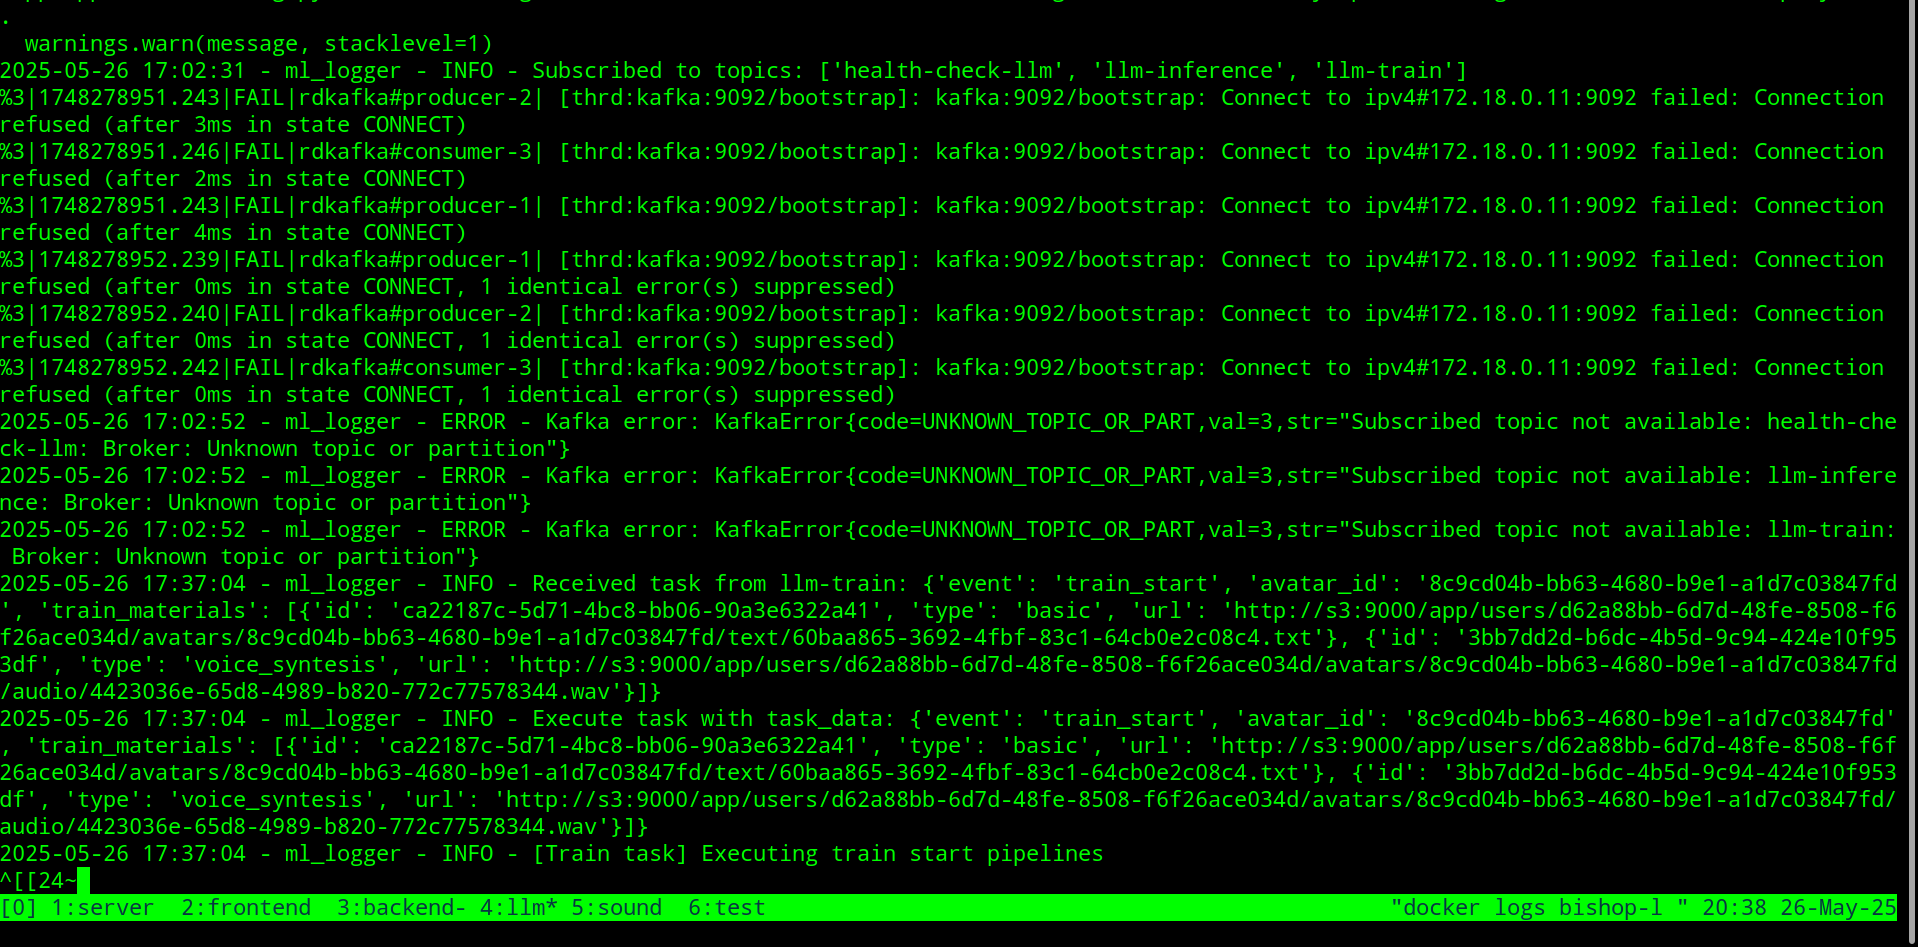
\includegraphics[width=1.0\linewidth]{images/results/llm-start-train.png}
    \caption{Запуск дообучения в модуле генерации текста}
    \label{fig:res-llm-start-train}
\end{figure}

\begin{figure}
    \centering
    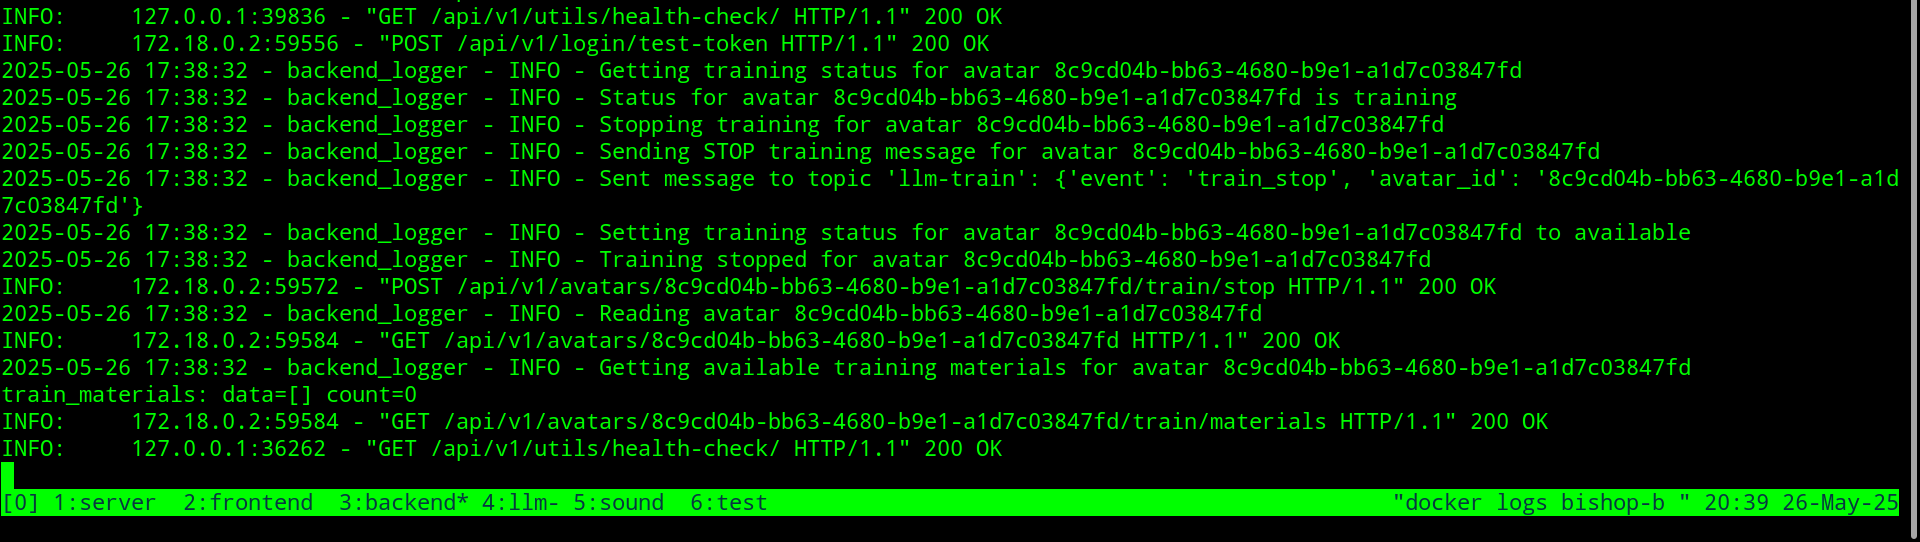
\includegraphics[width=1.0\linewidth]{images/results/bk-stop-train.png}
    \caption{Завершение обучения на стороне backend и обновление статуса}
    \label{fig:res-bk-stop-train}
\end{figure}

\begin{figure}
    \centering
    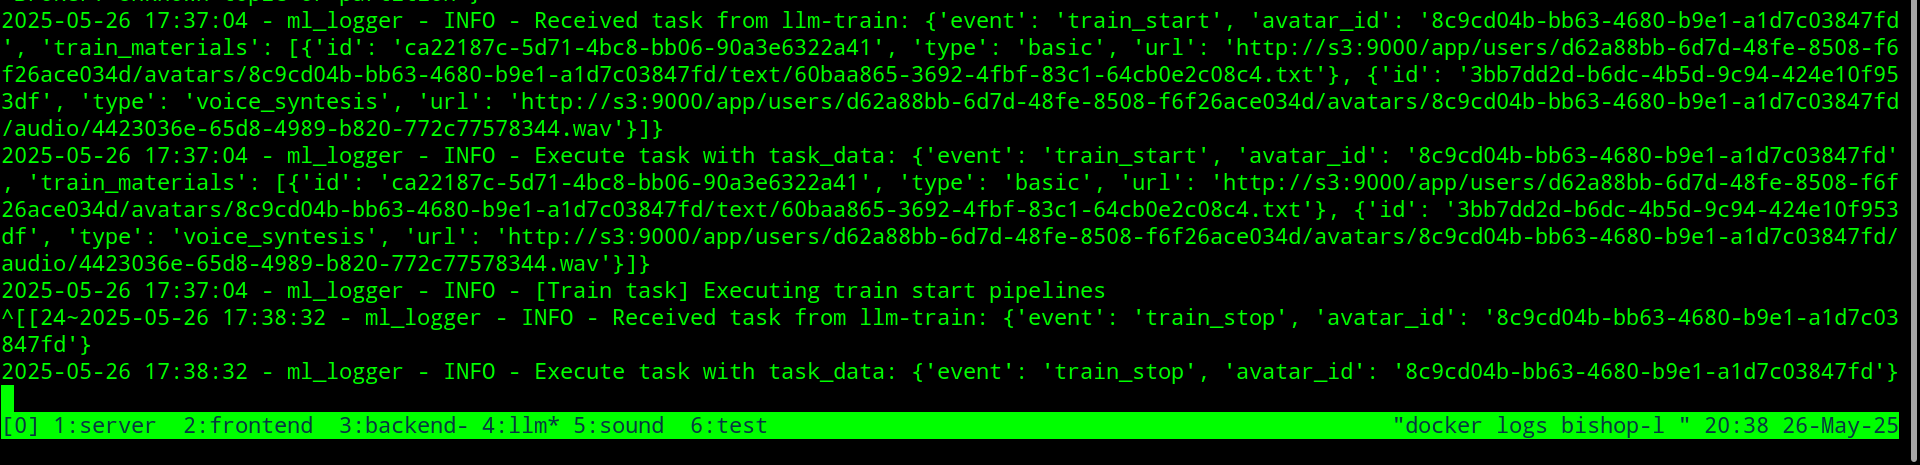
\includegraphics[width=1.0\linewidth]{images/results/llm-stop-train.png}
    \caption{Окончание дообучения модели генерации текста}
    \label{fig:res-llm-stop-train}
\end{figure}

\begin{figure}
    \centering
    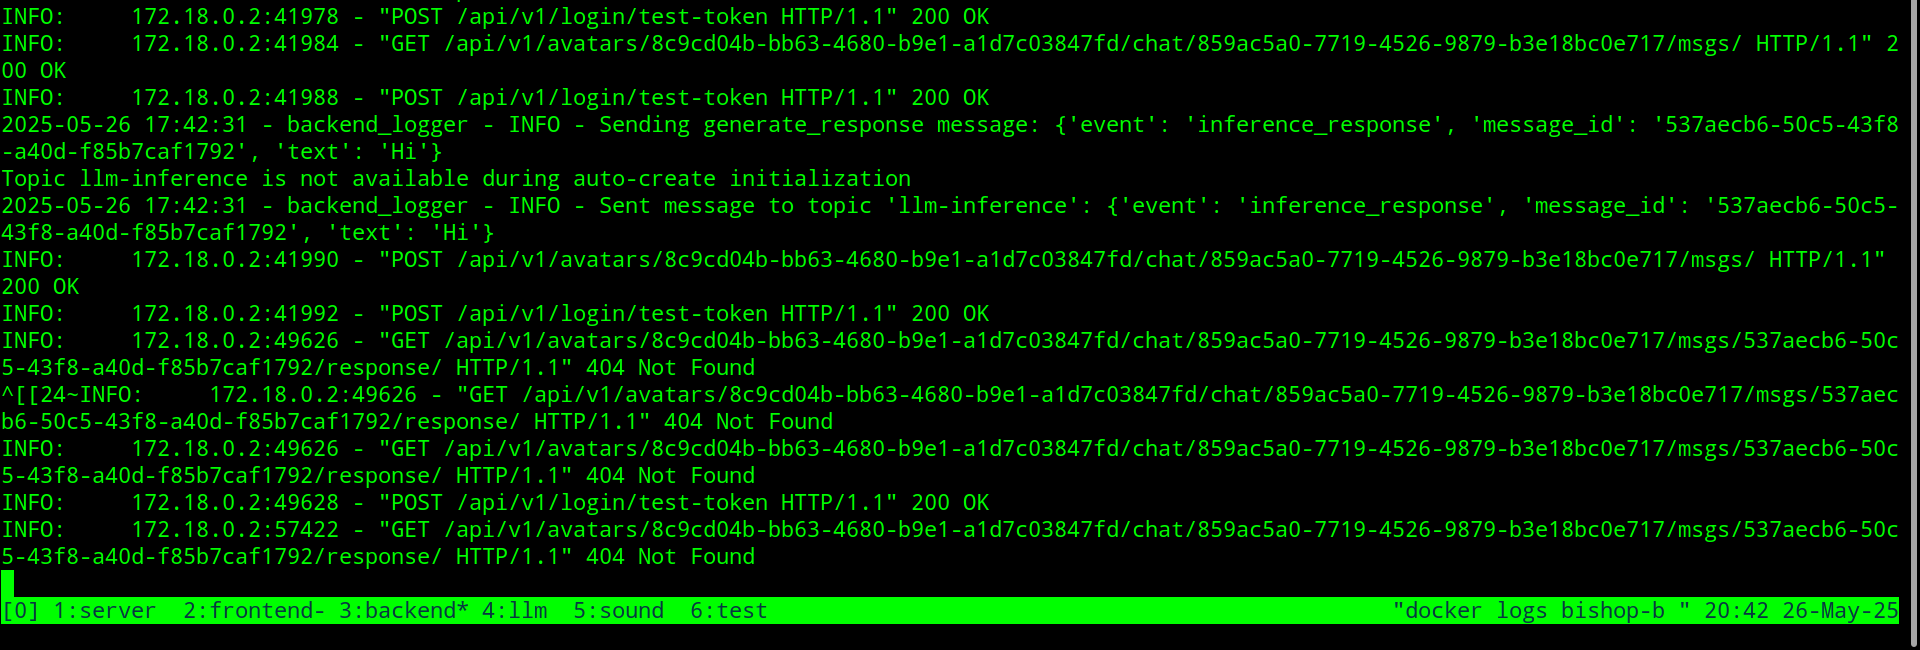
\includegraphics[width=1.0\linewidth]{images/results/bk-start-gen-llm.png}
    \caption{Отправка пользовательского сообщения и генерация текста}
    \label{fig:res-bk-start-gen-llm}
\end{figure}

\begin{figure}
    \centering
    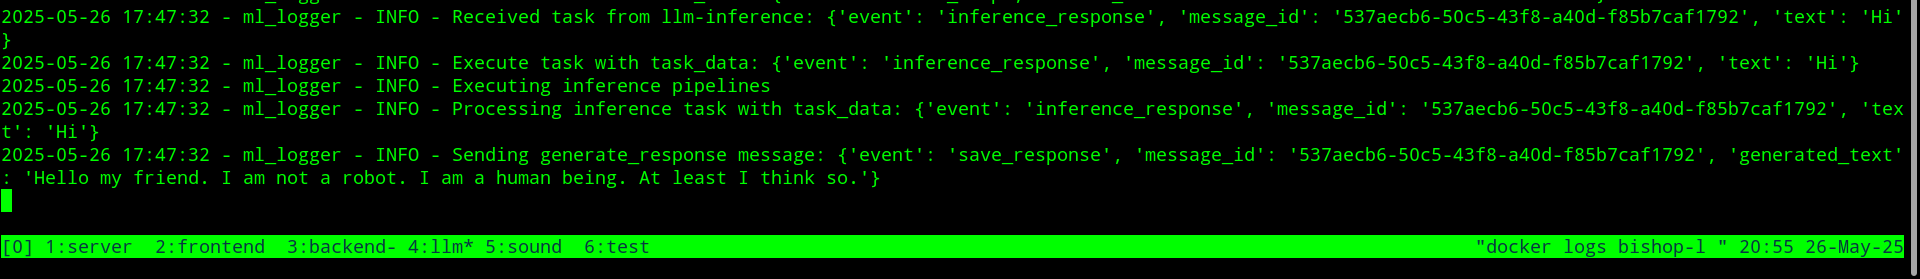
\includegraphics[width=1.0\linewidth]{images/results/llm-inference.png}
    \caption{Генерация ответа llm-моделью по заданному сообщению}
    \label{fig:res-llm-inference}
\end{figure}

\begin{figure}
    \centering
    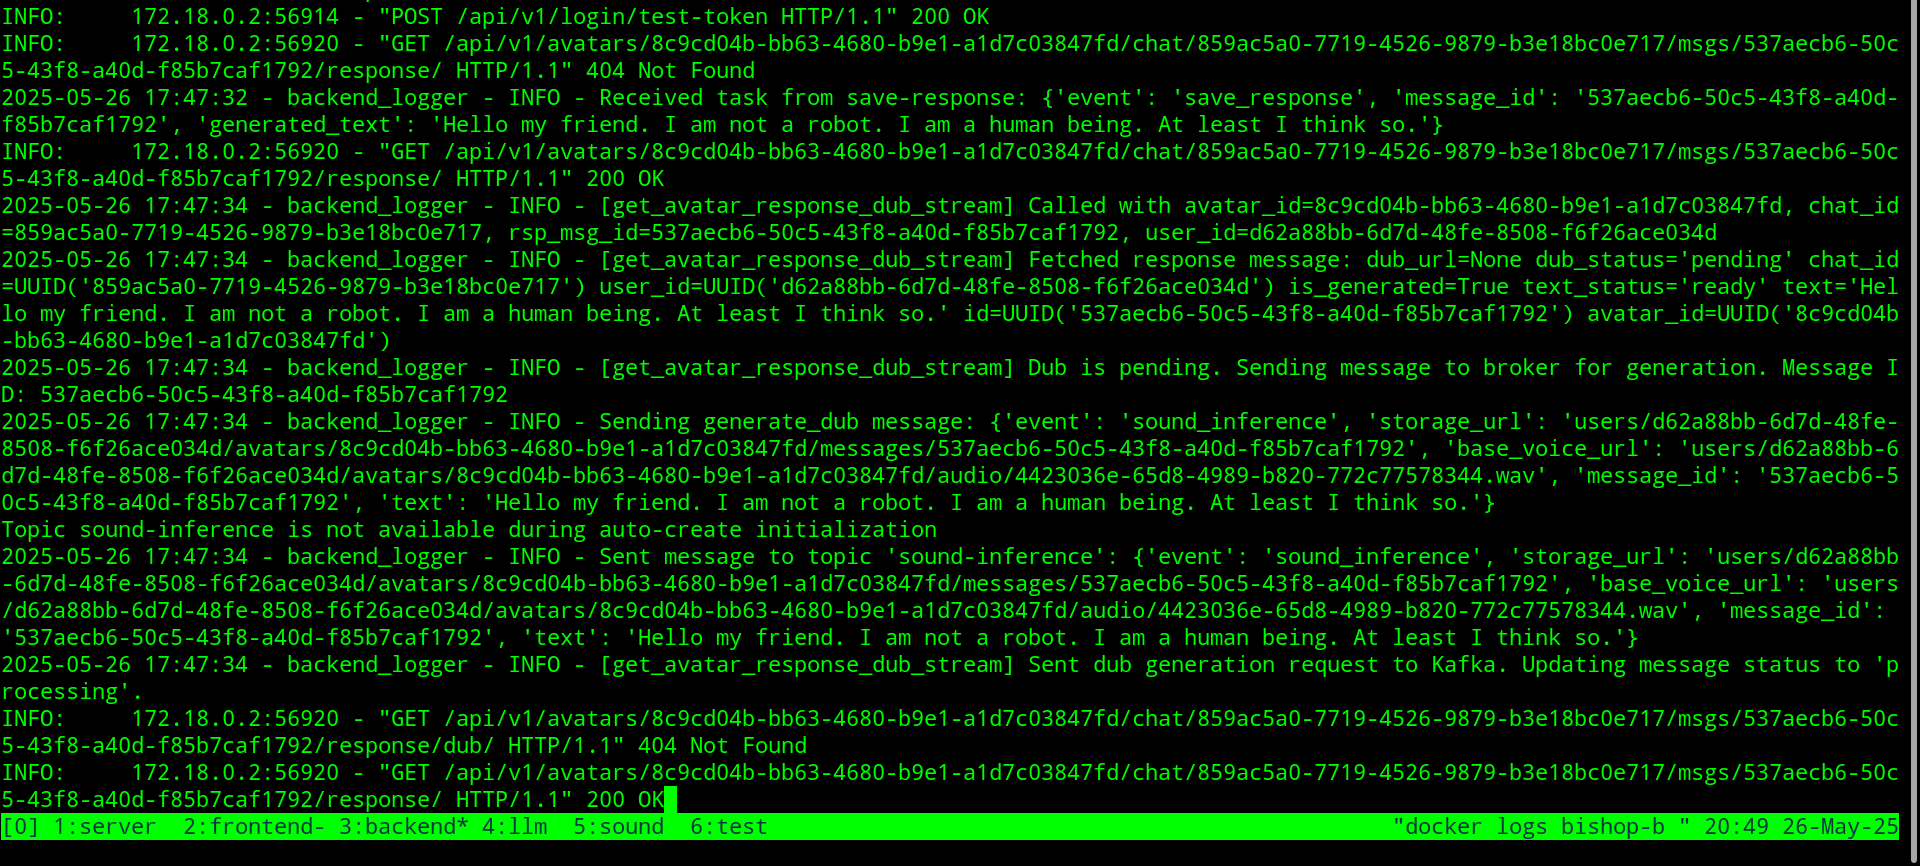
\includegraphics[width=1.0\linewidth]{images/results/bk-middle-gen-llm-done.png}
    \caption{Обработка сгенерированного текста и подготовка к озвучке}
    \label{fig:res-bk-middle-gen-llm-done}
\end{figure}

\begin{figure}
    \centering
    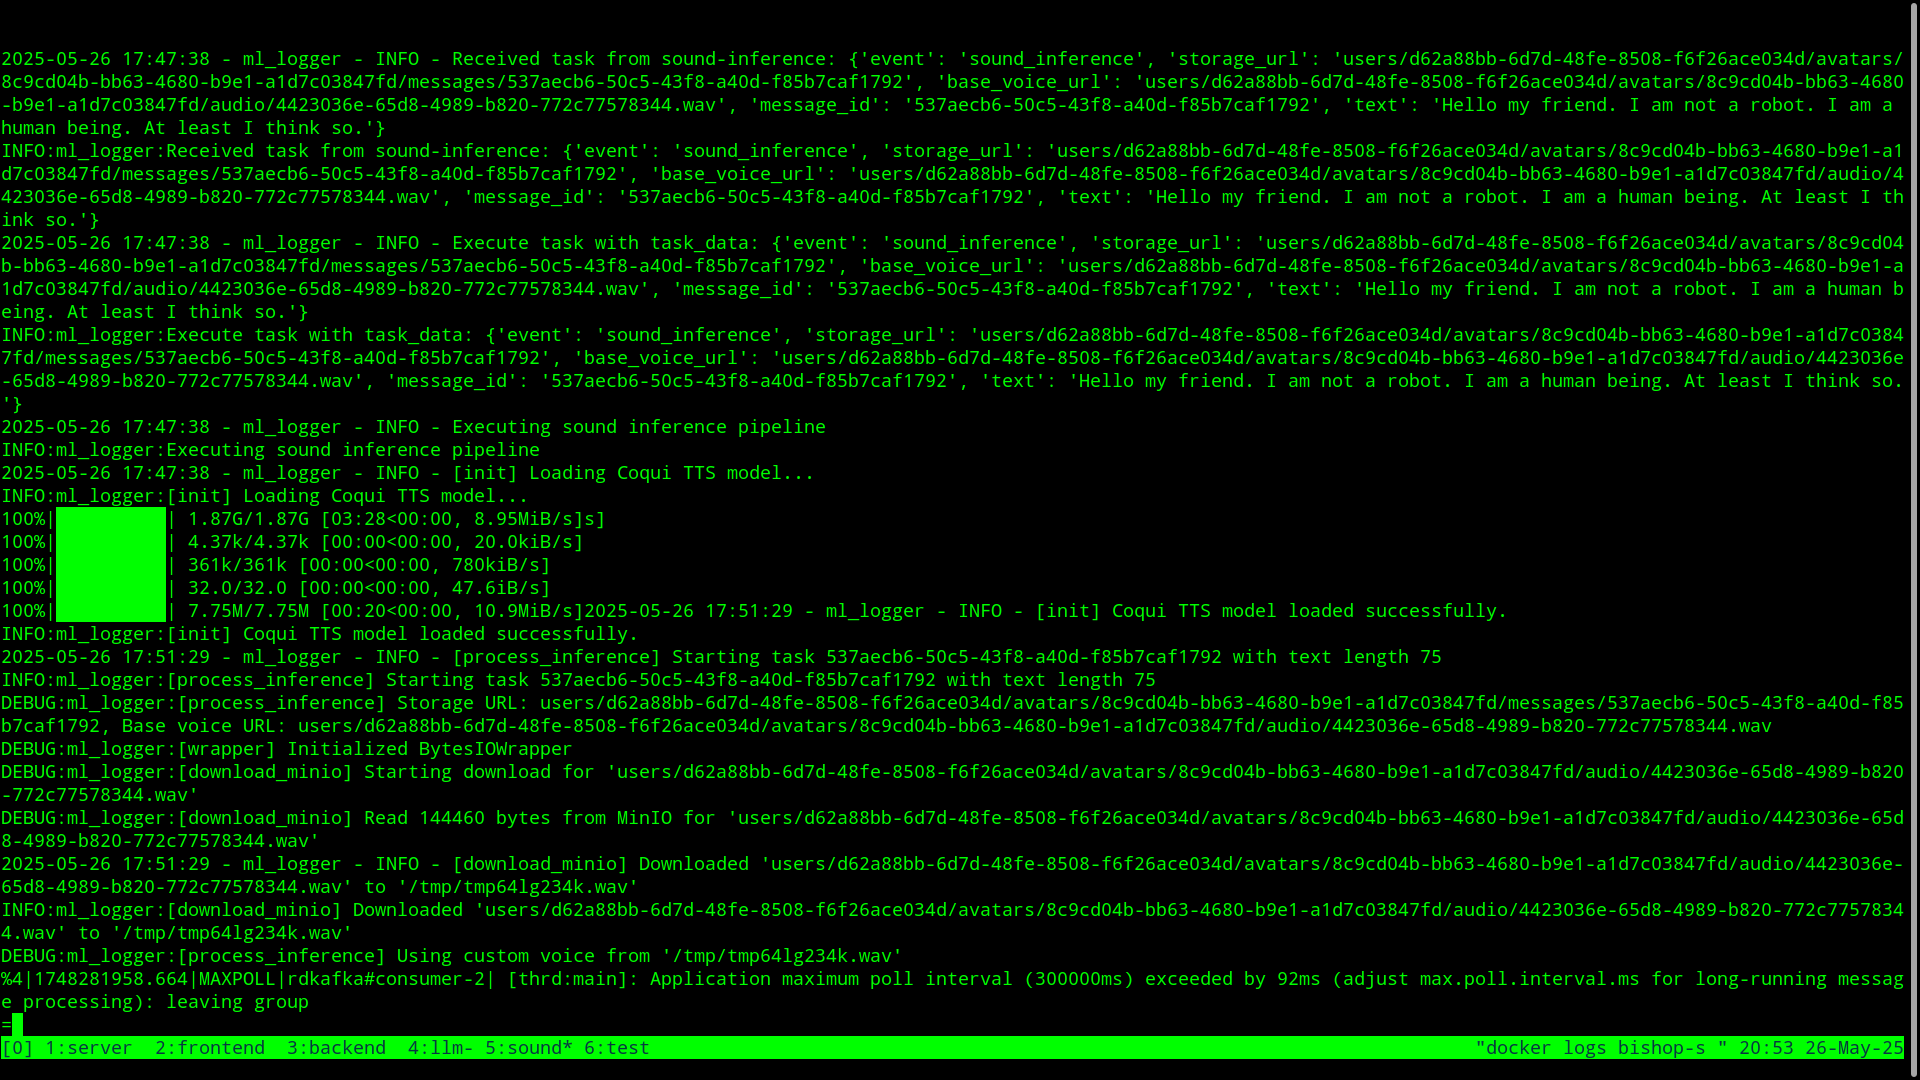
\includegraphics[width=1.0\linewidth]{images/results/sound-inference.png}
    \caption{Генерация аудиофайла на основе текста в сервисе озвучивания}
    \label{fig:res-sound-inference}
\end{figure}

\begin{figure}
    \centering
    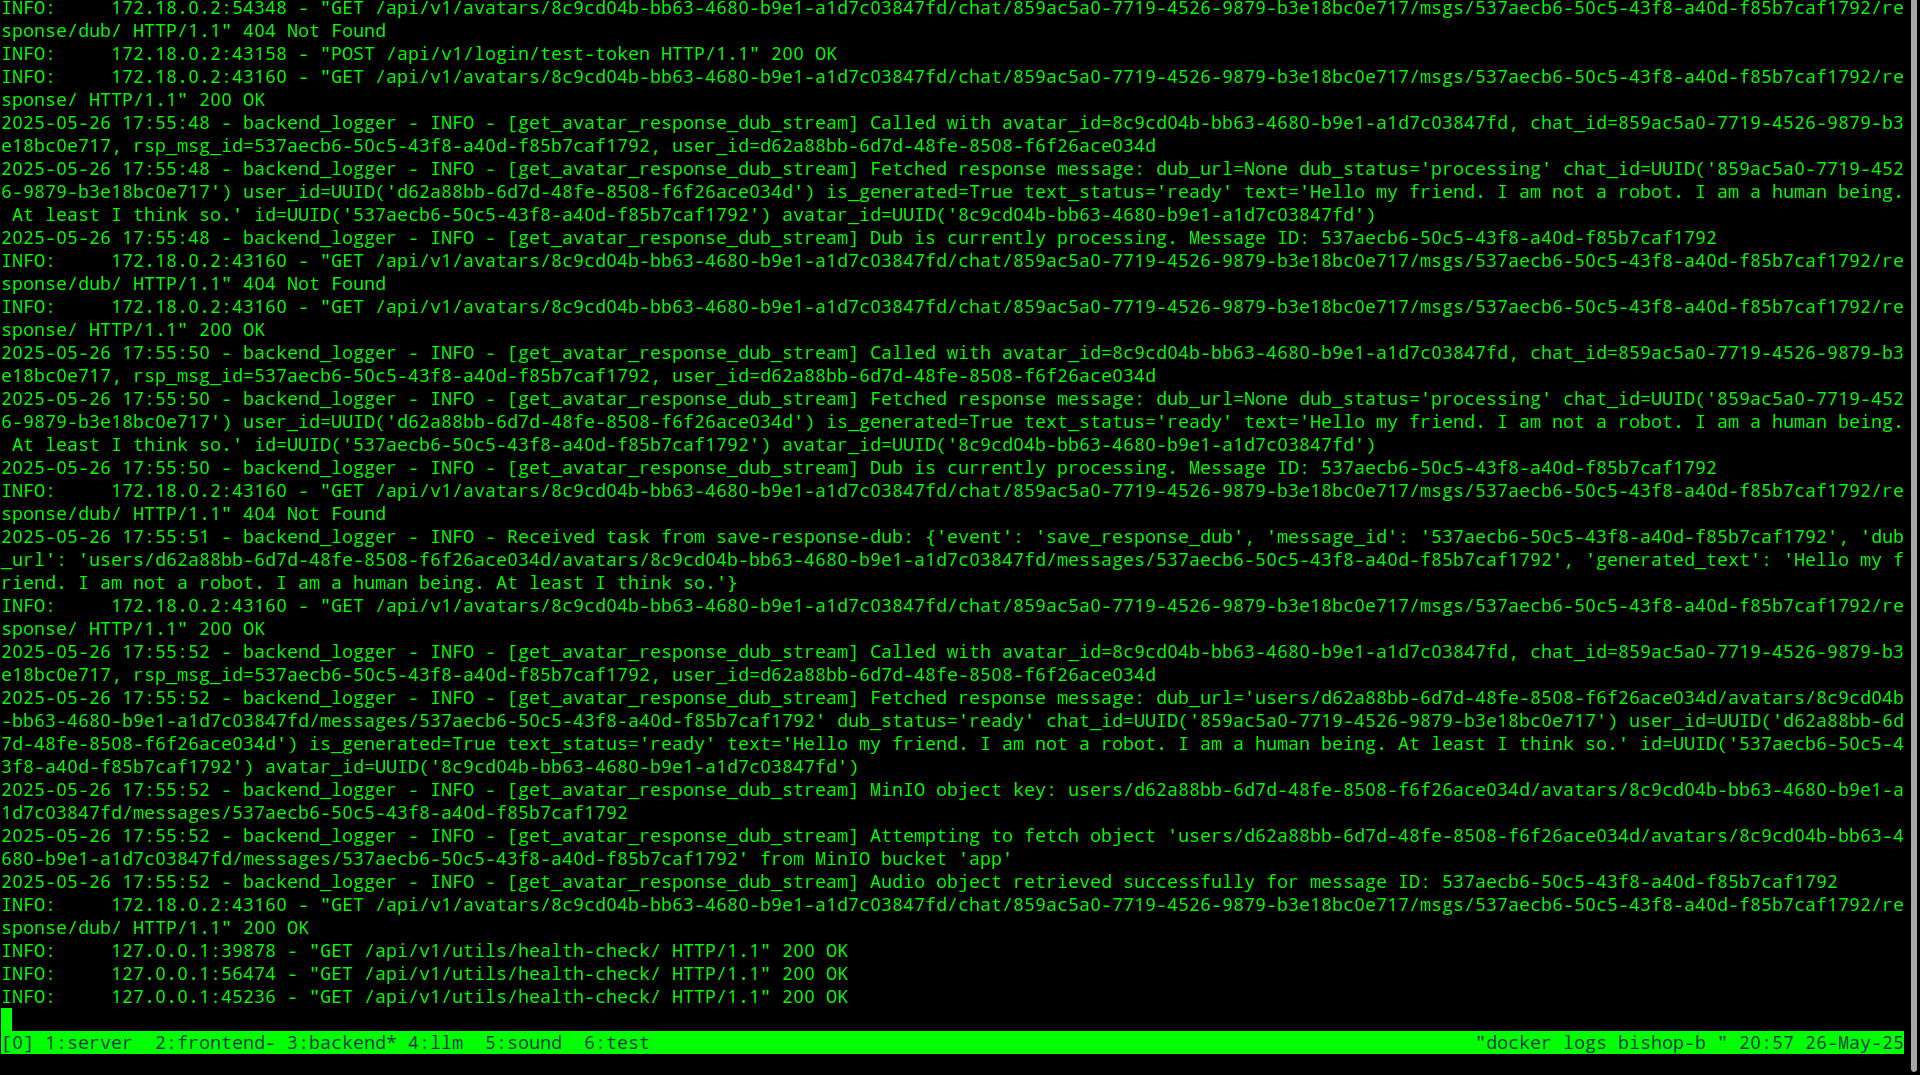
\includegraphics[width=1.0\linewidth]{images/results/bk-end-inference.png}
    \caption{Завершение ответа: возврат текста и аудио пользователю}
    \label{fig:res-bk-end-inference}
\end{figure}

\end{document}
